% AU template last modified by AU: 2010 Jul 02
% SH modifications for Markdown made in September 2018

\documentclass[12pt,econ]{sources/authesis}
\usepackage{natbib}  % natbib citation style
% The following packages are for the LaTeX generated graph
\usepackage{threeparttable}
\usepackage{tikz}
\usetikzlibrary{arrows}
\usepackage{tikz}
\usepackage{lscape}
\usepackage[hidelinks]{hyperref}
\usepackage{float} % to float tables
\usepackage{longtable} % for tables that are longer than one page
\usepackage{booktabs} % for stuff like \bottomrule in tables
\usepackage{adjustbox} % for \resizebox for tables
\usepackage{dcolumn} % to align on the decimal point of numbers in table columns
\usepackage{bm} % to make math symbols bold with \bm{}
\usepackage{changepage} % for \adjustwidth
\usepackage{amsfonts} % for math symbol "mathfrak"

% next 11 lines to create math symbol "reallywidehat"
\usepackage{scalerel,stackengine}
\stackMath
\newcommand\reallywidehat[1]{%
\savestack{\tmpbox}{\stretchto{%
  \scaleto{%
    \scalerel*[\widthof{\ensuremath{#1}}]{\kern-.6pt\bigwedge\kern-.6pt}%
    {\rule[-\textheight/2]{1ex}{\textheight}}%WIDTH-LIMITED BIG WEDGE
  }{\textheight}% 
}{0.5ex}}%
\stackon[1pt]{#1}{\tmpbox}%
}


%%-------------------------------------------------
%% For flowchart(s)
%%-------------------------------------------------

\usepackage{tikz}
\usetikzlibrary{shapes,arrows,positioning}

% Define block
\tikzstyle{block} = [rectangle, draw, fill=blue!20, text width=1cm, text centered, rounded corners, minimum height=3em]

% Define another block
\tikzstyle{block2} = [rectangle, draw, fill=blue!20, text width=2cm, text centered, rounded corners, minimum height=3em]

% Define yet another block
\tikzstyle{block3} = [rectangle, draw, fill=blue!20, text width=3cm, text centered, rounded corners, minimum height=3em]

% And another block
\tikzstyle{block4} = [rectangle, draw, text width=3cm, text centered, rounded corners, minimum height=3em]

% Define cloud
\tikzstyle{cloud} = [draw, ellipse, fill=red!20, node distance=1cm, minimum height=3em]

% Define another cloud
\tikzstyle{cloud2} = [draw, ellipse, node distance=1cm, minimum height=3em]

% Define line
\tikzstyle{line} = [draw, -latex', node distance = 0.1cm, auto]


% 
% FIGURES
%
\usepackage{graphicx}
% SH: The following generates all images so they have a width \maxwidth. This means that they will get their normal width if they fit onto the page, but are scaled down if they would overflow the margins:
\makeatletter
\def\maxwidth{\ifdim\Gin@nat@width>\linewidth\linewidth
\else\Gin@nat@width\fi}
\makeatother
\let\Oldincludegraphics\includegraphics
\renewcommand{\includegraphics}[1]{\Oldincludegraphics[width=\maxwidth]{#1}}
% SH: The following is repeated from the .cls file to make it appear in Markdown. The commands set the figure float, count etc.
\makeatletter
\def\fps@figure{ht} 
\def\ftype@figure{1}
\def\ext@figure{lof}
\def\fnum@figure{\figurename~\thefigure}
\def\figure{\@float{figure}}
\let\endfigure\end@float
\@namedef{figure*}{\@dblfloat{figure}}
\@namedef{endfigure*}{\end@dblfloat}
\makeatother
% SH: The following is repeated from the .cls file to make it appear in Markdown. The commands set the captions and also make the lof and lot double-spaced (unless it extends to more than one line, in which case it's single-spaced)
\makeatletter
\def\caption{\refstepcounter\@captype \@dblarg{\@caption\@captype}}
\long\def\@caption#1[#2]#3{%
  \par \par
  \addcontentsline{\csname ext@#1\endcsname}{#1}%
    {\protect\numberline{\csname the#1\endcsname.}{\ignorespaces #2}}%
  \addtocontents{\csname ext@#1\endcsname}{\protect\addvspace{10\p@}}%
  \begingroup
    \@parboxrestore
    \if@minipage
      \@setminipage
    \fi
    \normalsize
    \itshape % SH: Added \itshape myself for aesthetics -- to distinguish figure caps from text
    \@makecaption{\csname fnum@#1\endcsname}{\ignorespaces #3}\par
  \endgroup}
\makeatother
% end SH



% Declarations for Front Matter
%
% IMPORTANT: IF A TITLE OR SUBTITLE EXCEEDS MORE THAN ONE LINE,
%            THERE SHOULD ONLY BE  48 CHARACTERS PER LINE.
%
% The dissertation title must be capitalized for AU-CAS

\title{WHAT THE PEOPLE THINK: ADVANCES IN PUBLIC OPINION MEASUREMENT USING MODERN STATISTICAL METHODS}
\author{Simon Heuberger}
\degreeyear{2020}
\degree{Doctor of Philosophy}
\chair{Professor Jeff Gill}
\secondreader{Professor Ryan T. Moore}
\thirdreader{Professor Elizabeth Suhay}
\fourthreader{Professor R. Michael Alvarez}
\degreefield{Government}

\begin{document}

\maketitle

\maketitle

% The following command makes the copyright page

\copyrightpage

% The frontmatter environment uses roman lower case page numbering. The
% abstract, acknowledgements, table of contents, list of figures, and
% list of tables are a part of this environment.
\begin{frontmatter}

% The Guide requires one numbered abstract page.
% The 'abstractn' macro generates a numbered abstract page.
% Do NOT use the 'abstract' macro, which generates an unnumbered, abstract page.
% (NOTE: The Guide no longer requires two abstract pages, one numbered, one without numbers.)

\abstractn{Surveys are a central part of political science. Without surveys, we would not know what people think about political issues. Survey experiments further enable us to test how people react to given treatments. Surveys and survey experiments are only as good as the measurements and analytical techniques we as researchers employ, though. For one particular survey variable called ordinal variables, some of our current measurements and techniques are insufficient. Ordinal variables consist of ordered categories where the spacing between each category is uneven and not known. Ordinal variables are highly important because the most important predictor of political behavior is an ordinal variable: education. Ordinal example categories for education could be ``Some High School'', ``High School Graduate'', and ``Bachelor's Degree''. The literature currently often does not take the special nature of ordinal variables, i.e.~their uneven spacing, into account. This could misrepresent the data and potentially distort survey results. It is important that we measure and use education and other ordinal variables correctly. My dissertation develops two methods to do so and applies them in original survey research. Chapter II develops a new method to improve the use of ordinal variables in the assignment of treatment in survey experiments. Chapter III develops a new method to treat missing survey data with ordinal variables. Chapter IV applies both methods in an online survey experiment on political framing.}

%This is an abstractn.  There are page numbers.
%The \emph{Guide} says an abstract should not exceed 350 words.
%(If you do exceed this,
%then under the CAS option, the first page is numbered bottom center, and %the rest are numbered top right.)


% Acknowledgements are optional. If you do not wish to include them,
% simply do not include this command in your source.

\acknowledgements{I want to thank Fendi and Muesli, the two greatest creatures on the planet. And of course Waldemar Burgo.}


\listoftables

\listoffigures

\tableofcontents


\end{frontmatter}

\hypertarget{introduction}{%
\chapter{INTRODUCTION}\label{introduction}}

This is the introduction.

\hypertarget{ordblock}{%
\chapter{PRECISION IN SURVEY EXPERIMENTS -- A NEW METHOD TO IMPROVE BLOCKING ON ORDINAL VARIABLES}\label{ordblock}}

\hypertarget{ordblock-intro}{%
\section{Introduction}\label{ordblock-intro}}

Survey experiments collect background information and attempt to uncover treatment effects on public opinion and/or behavior. In order to identify such potential effects, the treatment groups need to be comparable. All treatment groups need to look the same in every measure, i.e.~they must be balanced. This can be achieved through random assignment of participants to treatment groups. Randomization, i.e.~flipping a coin to decide which treatment group a participant is assigned to, probabilistically results in balance based on the Law of Large Numbers (Urdan, 2010). For small samples, however, it can lead to serious imbalance. It can easily be that the treatment groups will not look the same. This can leave experimental results in statistically murky waters (Fox, 2015; Imai, 2018; King, Keohane, \& Verba, 1994). In survey experiments, the overall sample size is often split across several treatment groups, which can exacerbate the problem. Chong \& Druckman (2007), for instance, split 869 participants in a framing experiment on urban growth over 17 treatment groups, which leads to an average of just over 50 participants per group. Randomization is unlikely to lead to balanced treatment groups of this size. Researchers need to employ statistical methods to obtain balanced groups here. Blocking, i.e.~arranging participants in groups that are equal in terms of participants' covariates and using random allocation within these groups, can alleviate such worries.

Blocking depends on covariates. In political science, many covariates with high predictive power are categorical variables, i.e.~variables where the data can be divided into groups. These include interval (ordered and evenly spaced, e.g.~\texttt{Income}) and ordinal (ordered and unevenly spaced, e.g.~\texttt{Education}) variables. To block, these variables are often made numeric, e.g.~by assigning the numbers 1-4 to the variable categories. This is acceptable for interval variables as the evenly spaced numbers correspond to the evenly spaced categories. For ordinal variables, however, this can be problematic. An arbitrary evenly spaced string of numbers does not correspond to the unevenly spaced ordinal categories and may misrepresent the data. I propose an ordered probit threshold approach to circumvent this problem: This approach estimates an assumed underlying latent continuous structure underneath ordinal variables whose data-driven categories can then be used for blocking. By training a linear model on meaningful data, it creates numerical thresholds which partition the variable into regions corresponding to the ordinal categories and bins the observations between these thresholds according to the explanatory variables. These binned cases determine which of the original categories make sense given the underlying latent continuous structure. The result is a data-based and non-arbitrary re-estimated set of variable categories. Because of their data-driven estimation, these categories can be safely used for blocking. This approach allows researchers to block on ordinal variables in survey experiments without making unwarranted assumptions in terms of arbitrary numeric values whilst fully utilizing the ordinal information provided and respecting uneven spaces.

The following sections provide a background on survey experiments and blocking, describe the key aspects of ordinal variables, and outline my proposed ordered probit approach. I then demonstrate the benefits and implications of this approach with external survey data and original data from an online survey experiment. Since there currently is no available tool to block in online survey experiments, I create my own survey environment in \texttt{shiny}, which will be described in more detail below.

\hypertarget{ordblock-theory}{%
\section{Theory}\label{ordblock-theory}}

\hypertarget{ordblock-theory-experiments}{%
\subsection{Preliminary Notations on Survey Experiments}\label{ordblock-theory-experiments}}

The simplest of survey experiments has two potential outcomes for participants \(i\), \(y_{1i}\) and \(y_{0i}\), with 1 denoting the treatment and 0 referring to the control. Consider a simplified version of a famous survey experiment by Tversky \& Kahneman (1981), where researchers want to test the effect of the mortality format on participants' choices. They provide participants with the following scenario:

\vspace{0.3cm}
\begin{adjustwidth}{50pt}{50pt}
\ssp
\noindent Imagine that the US is preparing for the outbreak of an unusual Asian disease, which is expected to kill 600 people. A program to combat the disease has been proposed. Assume that the exact scientific estimates of the consequences of the program are as follows...
\end{adjustwidth}
Participants in the control group receive the program description in survival format:

\vspace{0.3cm}
\begin{adjustwidth}{50pt}{50pt}
\ssp
\noindent If the program is adopted, 200 out of 600 people will live.
\end{adjustwidth}
Participants in the treatment group receive the program description in mortality format:

\vspace{0.3cm}
\begin{adjustwidth}{50pt}{50pt}
\ssp
\noindent If the program is adopted, 400 out of 600 people will die.
\end{adjustwidth}
All participants are subsequently asked whether they support or oppose the program. The treatment effect for each individual participant \(i\) is given by \(y_{1i} - y_{0i}\). If both groups of participants look the same regarding their covariates (\texttt{Age}, \texttt{Education}, \texttt{Income} etc.), a comparison of the groups' average support reveals the Average Treatment Effect (ATE) across all participants, \(\mathbf{E}[\delta] = \mathbf{E}[y_{1i} - y_{0i}]\). A central characteristic of such a comparison is the fundamental problem of causal inference (Holland, 1986; Rubin, 1974): We are unable to observe both potential outcomes for the same participant at once. In our case, we cannot observe how much participant A supports the program if given the survival format whilst also observing how much the same participant A would have supported the program if given the mortality format. If we could, it would be simple to calculate the true average treatment effect, \(\mathbf{E}[\delta] = \mathbf{E}[y_{1i}|T=1] - \mathbf{E}[y_{0i}|T=0]\), with \(T=0\) denoting the control and \(T=1\) the treatment group. Since the true average treatment effect is unobservable, we need to use statistical means to assess the counterfactuals. This can be done by balancing the treatment and control groups. If both groups of participants look the same in every measure, we can use the participants who received the mortality format (treatment) to estimate what would have happened to the participants who did not receive the mortality format (control). The crucial aspect is whether the two groups do indeed look the same in terms of participants' covariates. The potential outcome of the control needs to mirror what would have happened in the case of treatment, and vice versa. There are two main means by which this may be achieved: Randomization and blocking.

\hypertarget{ordblock-theory-randomization}{%
\subsection{Randomization}\label{ordblock-theory-randomization}}

Randomization is equivalent to flipping a coin for each participant to be assigned to treatment or control. This chance procedure gives each participant an equal chance of being assigned to either group (or groups, in case of multiple treatment groups) (Lachin, 1988). Randomization increases covariate balance as the number of participants, \(n\), increases (Imai, King, \& Nall, 2009). The larger a researcher's sample, the better the resulting balance from randomization in expectation. Probabilistically, randomization enables the comparison of the average treatment effect to be unbiased, which allows the researcher to attribute any treatment effects to the treatment (King et al., 2007).

While randomization thus guarantees balance as the sample size reaches infinity, it often does not do so in the naturally finite sample sizes researchers actually work with. With huge samples, the Law of Large Numbers predicts that treatment groups selected through randomization will be balanced. With small samples, however, it is possible to get unlucky and end up with unbalanced groups (Imai, King, \& Elizabeth A. Stuart, 2008). Blocking can help achieve balance in such scenarios (Epstein \& King, 2002).

\hypertarget{ordblock-theory-blocking}{%
\subsection{Blocking}\label{ordblock-theory-blocking}}

Identical levels in terms of covariates across treatment groups represent the key aspect in experimental studies. In randomization, this is achieved by random chance. In blocking, this is achieved by combining covariate information about the participants with randomization. Specifically, participants are blocked into treatment groups that are similar to one another in terms of the their covariates before treatment is assigned. Their similarity is estimated with the Mahalanobis or Euclidian distance. Blocking is better suited to achieving balance in finite samples than randomization, as it ``directly controls the estimation error due to differing levels of observed covariates in the treatment and control groups'' (Moore, 2012, p. 463). This is particularly relevant with small samples and a high number of treatment groups, as the overall number of participants needs to be divided up. Figures \ref{BoxLawLarNum} and \ref{HistLawLarNum} show this visually. A numeric discrete variable with levels 1 to 5 is randomized and blocked for different sample sizes and numbers of treatment groups. This is repeated 100 times for each sample size. Figure \ref{BoxLawLarNum} shows the maximum distances between treatment groups across these repetitions for sample sizes up to 1,000 for two, three, five, and ten treatment groups. Blocking outperforms randomization in every scenario. The difference between the two methods is smallest for large samples and a small number of treatment groups.
\begin{figure}
\centering
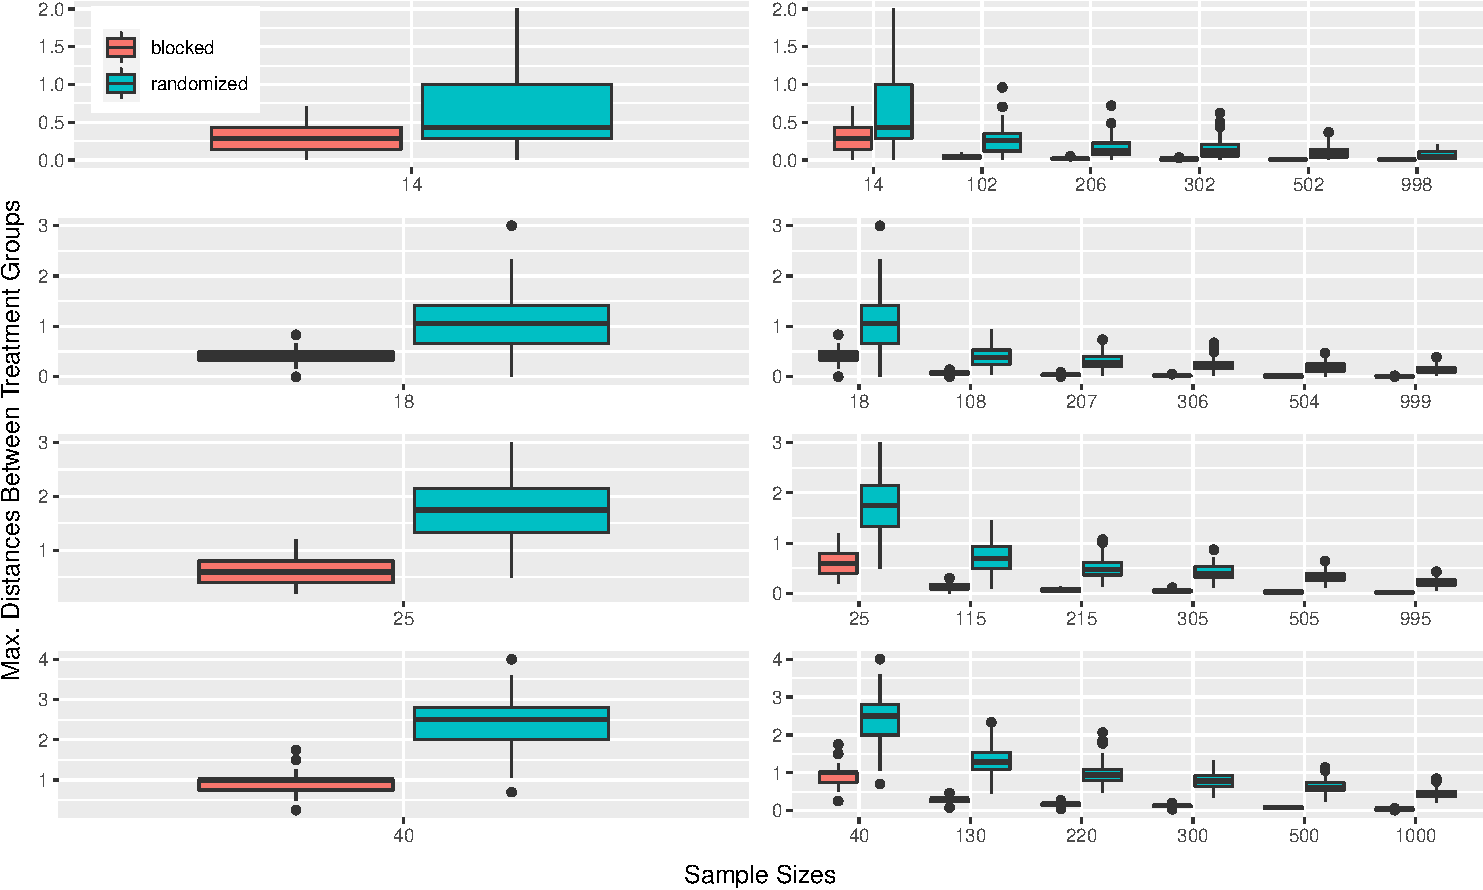
\includegraphics{dissertation_files/figure-latex/Boxplot-Law-Large-Numbers-1.pdf}
\caption{\label{fig:Boxplot-Law-Large-Numbers}Distances between treatment group means in randomized and blocked data. Increasing sample size for 2 (top row), 3 (second row), 5 (third row), and 10 treatment groups (bottom row). Leftmost pair on right panel is exactly the pair on the left panel\label{BoxLawLarNum}}
\end{figure}
For \(n = 998\) and two treatment groups, the largest distance between randomized treatment groups is 0.208, and the largest distance between blocked treatment groups is 0.01. For small samples and a large number of treatment groups, however, the difference is much starker. For \(n = 40\) and ten treatment groups, the largest distance between randomized treatment groups is 4, and the largest distance between blocked treatment groups is 1.75. Figure \ref{HistLawLarNum} shows the distribution of these imbalances.
\begin{figure}
\centering
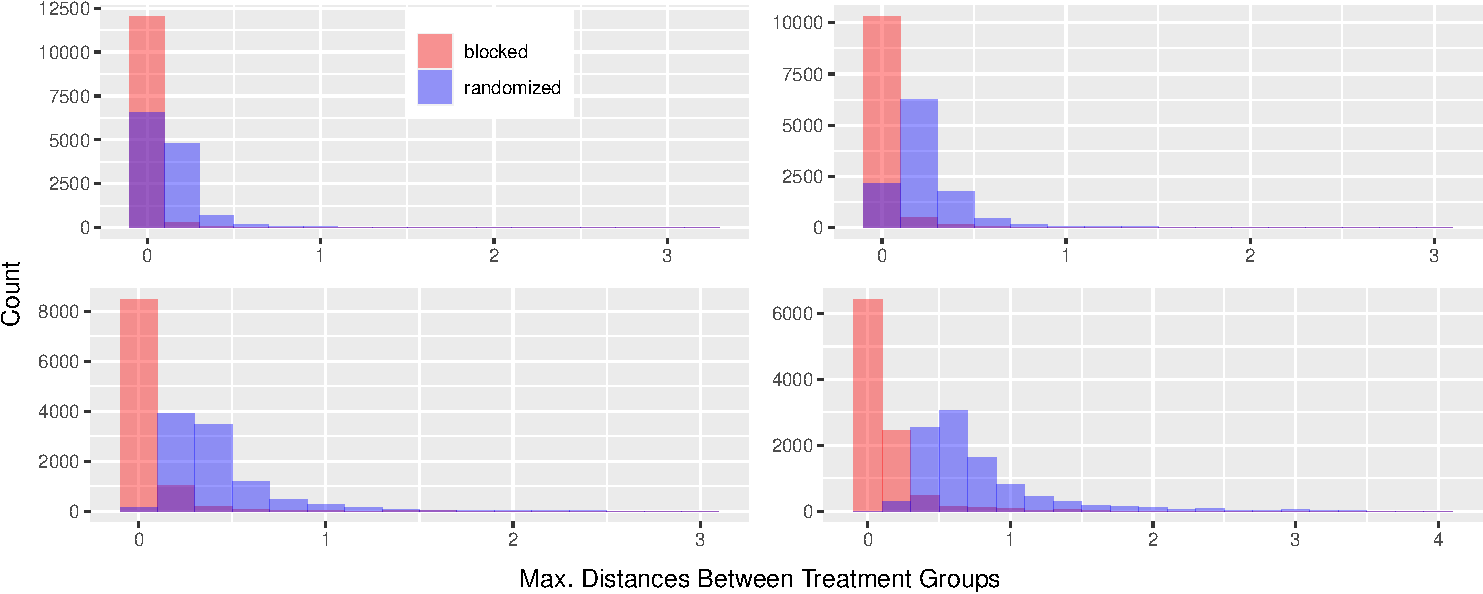
\includegraphics{dissertation_files/figure-latex/Hist-Law-Large-Numbers-1.pdf}
\caption{\label{fig:Hist-Law-Large-Numbers}Distribution of treatment group differences in randomized and blocked data for 2 (top left), 3 (top right), 5 (bottom left), and 10 (bottom right) treatment groups\label{HistLawLarNum}}
\end{figure}
\hypertarget{ordblock-theory-blocking-onthego}{%
\subsubsection{Blocking On The Go}\label{ordblock-theory-blocking-onthego}}

In political science, researchers often have an already-collected data set in front of them. One example would be the American National Election Studies (ANES), a pre-existing survey database, which is often used to analyze voter turnout (see for instance Jackman \& Spahn, 2018; Leighley \& Nagler, 2014), among many others. This setup means all covariate information on all participants is known at the time of assignment, which makes blocking straight-forward. Oftentimes, however, the covariate information of all participants is not known at the time of assignment. This is the case, for instance, for online survey experiments, where each participant completes the survey at differing times. Participants `trickle in' for treatment assignment as the experiment progresses. `Traditional' blocking can not be used here, since it relies on covariate information about the entire sample. Instead, we need to block continuously as the experiment progresses, or block `on the go'. This is called sequential blocking.

Sequential blocking in political science is based on covariate-adaptive randomization, which varies probabilities based on knowledge about previous participants and the current participant (Chow \& Chang, 2007). Traditional covariate-adaptive approaches, such as the biased coin design (Efron, 1971) and minimization (Pocock \& Simon, 1975), assign the incoming participant to the treatment group with the fewest participants with identical covariate information. This works for discrete covariates as the number of possible covariate levels is finite. For continuous covariates, the number of possible covariate levels rises exponentially. Participants are unlikely to look the same, and identical participants are rare. Blocking on continuous covariates is not possible with these traditional approaches (Eisele, 1995; Markaryan \& Rosenberger, 2010; Rosenberger \& Lachin, 2002). Moore \& Moore (2013) develop a method to do so by exploiting relationships between the current participant's covariate profile and those of all previously assigned participants. They define the similarity between participants with the Mahalanobis distance (MD) between participants \(q\) and \(r\) with covariate vectors \(\bm{x}_q\) and \(\bm{x}_r\): \newline \noindent \(MD_{qr} = \sqrt{(\bm{x}_q - \bm{x}_r)' \reallywidehat{\sum}^{-1} (\bm{x}_q - \bm{x}_r)}\). To aggregate pairwise similarity, they implement the mean, median, and trimmed mean of the pairwise MDs between the current participant and the participants in each treatment condition: Participants are indexed with treatment condition \(t\) using \(r \in \{1,...,R\}\). For each condition \(t\), an average MD between the current participant, \(q\), and the participants previously assigned, \(t\). If the distance in terms of MD for the incoming participant is 2 in the control and 5 for the treatment condition, the incoming participant looks more similar to the control condition. To set the probability of assignment, Moore \& Moore (2013) calculate the mean Mahalanobis distances for each incoming participant, \(q\), for all treatment conditions, \(t\), and sort the treatment conditions by these averages. Randomization is biased towards conditions with high scores. For each value of \(k\), with \(k \in \{2,3,...,6\}\), the condition with the highest average MD is then assigned a probability \(k\) times larger than all other assignment probabilities.

Blocking is thus possible when all covariate information is known at the time of assignment and when this information `trickles in' over time. Covariate information, however, is only one side of the coin. Researchers also need to take into consideration the characteristics of the variable to block on. Not all types of variables can and should be used the same way to be blocked on. Specifically, the current use of ordinal variables as blocking variables is somewhat problematic.

\hypertarget{ordblock-theory-ordinal}{%
\subsection{Ordinal Variables}\label{ordblock-theory-ordinal}}

Ordinal variables are part of the larger framework of categorical variables. Categorical variables represent types of data which are commonly divided into three groups: Nominal, interval, and ordinal variables. Nominal variables are categorical variables with two or more categories that are not intrinsically ordered. Examples include \texttt{gender} (Female, Male, Transgender etc.), \texttt{race} (African-American, White, Hispanic etc.), and \texttt{party\ ID} (Democrat, Republican, Independent) where the categories cannot be ordered sensibly into highest or lowest. Interval variables are ordered categorical variables with evenly spaced values. Examples include \texttt{income} (\$20,000, \$40,000, \$60,000, \$80,000 etc.), where the distance between \$20,000 and \$40,000 is the same as the distance between \$60,000 and \$80,000. Ordinal variables are ordered categorical variables where the spacing between values is not the same. Examples include \texttt{education} (Elementary school, Some high school, High school graduate etc.) where the distance between ``Elementary school'' and ``Some high school'' is likely different than the distance between ``High school graduate'' and ``Some college''. Each subsequent category has quantitatively more education than the previous, but the exact measure of the distance between the categories is unclear.

For blocking, the categories of nominal variables are often turned into binary variables. This manipulation does not impose any unnatural ordering onto the variable and thus does not require any theoretical assumptions. Interval variables are often made numeric, which is statistically sound. It makes sense to assign numeric values such as 1, 2, 3, and 4 to \texttt{income} categories of \$20,000, \$40,000, \$60,000, and \$80,000. The distance between each of these categories is identical between any adjacent pair and thus translates perfectly into the numeric values with equally identical distances. The distance between \$20,000 and \$40,000 is the same as the distance between 1 and 2. Ordinal variables are also often made numeric for blocking. This is problematic because of their unevenly spaced categories. If the \texttt{education} categories ``Elementary school'', ``Some high school'', and ``High school graduate'' were turned into the numeric values 1, 2, and 3, we would wrongly assume that the distances between the education categories correspond to these evenly spaced values. Do the numbers 1 to 3 really represent the distances between the categories? Perhaps the true spacing between some of the categories is so narrow they should not even be separate categories at all. We cannot answer this by making an arbitrary assumption that is not justified by the data. Alternatively, if ``Elementary school'', ``Some high school'', and ``High school graduate'' were turned into three separate dummy variables, we would wrongly assume that there is no ordering to these values. In both cases, important information would be lost, which could lead to a large degree of distortion (O'Brien, 1981). To truly use the ordinal nature of a variable, we need to use both its quantitative and its inherent unevenly spaced ordered aspects to make a more underlying description of the data possible (Agresti, 2010). To fill this gap, I borrow from machine learning, which has close connections to problems of causal inference (Grimmer, 2015), and propose an ordered probit model that estimates an ordinal variable's underlying latent continuous structure and is trained on external data.

\hypertarget{ordblock-theory-op}{%
\subsection{Ordered Probit Approach}\label{ordblock-theory-op}}

Many approaches in the literature on the analysis of ordinal variables incorporate the distribution of the variable categories (Agresti, 1996). The most promising suggestions focus on natural extensions of probit and logit models (Winship \& Mare, 1984) by assigning scores to be estimated from the data (Agresti, 1990) and quantifying each non-quantitative variable according to the empirical distributions of the variable, assuming the presence of a continuous underlying variable for each ordinal indicator (Lucadamoa \& Amenta, 2014). In fact, Agresti (2010) states ``that the type of ordinal method used is not that crucial'' but that the ``results may be quite different, however, from those obtained using methods that treat all the variables as nominal'' (p.~3). The same applies to methods which treat ordinal variables as interval (Gertheiss \& Tutz, 2008). This suggests that a probit or logit model is suitable to uncover the latent continuous variable underlying an ordinal variable, thus using the ordinal information provided and respecting uneven distances. In the literature, this approach is focused exclusively on the analysis of ordinal variables as a response variable. I propose an ordered probit model that applies to ordinal variables as a predictive variable.

Let there be \(\bm{X}\), an \(n \times k\) matrix of explanatory variables. Let further \(\bm{Y}\) be observed on the ordered categories \(\bm{Y}_i \in [1,\ldots,k]\), for \(i=1,\ldots n\), and let \(\bm{Y}\) be assumed to be produced by the unobserved latent continuous variable \(\bm{Y^*}\). \(\bm{Y^*}\) is continuous on \(\mathfrak{R}\) from \(-\infty\) to \(\infty\). The `response mechanism' for the \(r^{th}\) category is \(Y=r \Longleftrightarrow \theta_{r-1} < Y^* < \theta_r\). This requires there to be thresholds on \(\mathfrak{R}\):
\(Y^*_i: \; \theta_0 \underset{c=1}{\longleftarrow\!\longrightarrow} \theta_1 \underset{c=2}{\longleftarrow\!\longrightarrow} \theta_2 \underset{c=3}{\longleftarrow\!\longrightarrow} \theta_3\ldots \theta_{C-1} \underset{c=C}{\longleftarrow\!\longrightarrow} \theta_C\). The vector of (unseen) utilities across individuals in the sample, \(Y^*\), is determined by a linear model of explanatory variables: \(\bm{Y^*} = \bm{X} \bm{\beta} + \mathbf{E}\), where \(\bm{\beta} =[\beta_1,\beta_2,\ldots,\beta_p]\) does not depend on the \(\theta_j\) and \(\mathbf{E} \sim F_{\mathbf{E}}\). For the observed vector \(\bm{Y}\),
\begin{align*}
                     p(\bm{Y} \leq r|\bm{X}) &= p(\bm{Y^*} \leq \theta_r) = p(\bm{X}\bm{\beta} + \mathbf{E} \leq \theta_r)\\
                                      &= p(\mathbf{E} \leq \theta_r+\bm{X}\bm{\beta}) = F_{\mathbf{E}}(\theta_r + \bm{X}\bm{\beta})
            \end{align*}
is called the cumulative model because \(p(\bm{Y} \leq \theta_r|\bm{X}) = p(\bm{Y}=1|\bm{X}) + p(\bm{Y}=2|\bm{X}) + \ldots + p(\bm{Y}=r|\bm{X})\). A logistic distributional assumption on the errors produces the ordered logit specification: \(F_{\mathbf{E}}(\theta_r - \bm{X}'\bm{\beta}) = P(\bm{Y} \leq r|\bm{X}) = [1+\exp(-\theta_r-\bm{X}'\bm{\beta})]^{-1}\). The likelihood function is: \(L(\bm{\beta},\bm{\theta}|\bm{X},\bm{Y}) = \prod_{i=1}^{n}\prod_{j=1}^{C-1}\left[\Lambda(\theta_j + \bm{X}_i'\bm{\beta}) - \Lambda(\theta_{j-1} + \bm{X}_i'\bm{\beta}) \right]^{z_{ij}}\) where \(z_{ij}=1\) if the \(i^\text{th}\) case is in the \(j^\text{th}\) category, and \(z_{ij}=0\) otherwise. The thresholds on \(\mathfrak{R}\) partition the variable into regions corresponding to the ordinal categories. The linear model, \(Y^*\), bins the observations between these thresholds according to the linear predictors.

To use this ordered probit model for blocking, we need to estimate a linear combination of meaningful covariates as predictors and an ordinal variable as the dependent variable. We then train this model on externally and internally valid data. This estimates cutoff thresholds between the ordinal categories and bins data cases according to the linear predictors. The binned cases determine which variable categories make sense, given the underlying latent continuous variable. We then block on the resulting categories.

\hypertarget{ordblock-data}{%
\section{Data}\label{ordblock-data}}

\hypertarget{ordblock-data-opmodel}{%
\subsubsection{ANES Model Training}\label{ordblock-data-opmodel}}

One of the most common ordinal variables in political science is education. It is widely established that education represents one of the major driving forces behind public opinion and political behavior, such as turnout or donations, in the U.S. (Abramowitz, 2010; Dawood, 2015; Druckman, Peterson, \& Slothuus, 2013; Fiorina \& Abrams, 2009; Fiorina, Abrams, \& Pope, 2011; King, 1997; Leighley \& Nagler, 2014). One of the most respected and recognized externally and internally valid data sets are the American National Election Studies. I thus choose the following ordered probit model with the 2016 ANES data (the predictors are standard linear predictors in political science literature):

\vspace{-1cm}

\[Education \sim Gender + Race + Age + Income + Occupation + Party ID\]

When trained on the 2016 ANES data, this ordinal probit model estimates the thresholds between each of the education categories shown in Table \ref{education-categories}.
\begin{table}[!htbp] \centering 
  \caption{Ordered Probit Threshold Estimates} 
  \label{education-categories} 
\begin{tabular}{@{\extracolsep{5pt}} D{.}{.}{-3} D{.}{.}{-3} D{.}{.}{-3} D{.}{.}{-3} } 
\\[-1.8ex]\hline 
\hline \\[-1.8ex] 
\multicolumn{1}{c}{Thresholds} & \multicolumn{1}{c}{Coefficients} & \multicolumn{1}{c}{Standard Errors} & \multicolumn{1}{c}{t-values} \\ 
\hline \\[-1.8ex] 
\multicolumn{1}{c}{Up to 1st\textbar 1st-4th} & -7.869 & 1.024 & -7.681 \\ 
\multicolumn{1}{c}{1st-4th\textbar 5th-6th} & -7.146 & 0.717 & -9.965 \\ 
\multicolumn{1}{c}{5th-6th\textbar 7th-8th} & -5.379 & 0.326 & -16.515 \\ 
\multicolumn{1}{c}{7th-8th\textbar 9th} & -4.671 & 0.253 & -18.472 \\ 
\multicolumn{1}{c}{9th\textbar 10th} & -3.920 & 0.206 & -19.070 \\ 
\multicolumn{1}{c}{10th\textbar 11th} & -3.468 & 0.188 & -18.489 \\ 
\multicolumn{1}{c}{11th\textbar 12th} & -2.984 & 0.174 & -17.100 \\ 
\multicolumn{1}{c}{12th\textbar HS grad} & -2.511 & 0.166 & -15.116 \\ 
\multicolumn{1}{c}{HS grad\textbar Some college} & -0.710 & 0.154 & -4.607 \\ 
\multicolumn{1}{c}{Some college\textbar Associate} & 0.384 & 0.154 & 2.500 \\ 
\multicolumn{1}{c}{Associate\textbar Bachelor's} & 1.045 & 0.154 & 6.766 \\ 
\multicolumn{1}{c}{Bachelor's\textbar Master's} & 2.478 & 0.160 & 15.538 \\ 
\multicolumn{1}{c}{Master's\textbar Professional} & 4.099 & 0.177 & 23.144 \\ 
\multicolumn{1}{c}{Professional\textbar Doctorate} & 4.838 & 0.197 & 24.589 \\ 
\hline \\[-1.8ex] 
\end{tabular} 
\end{table}
The observations in the data are binned according to the estimated threshold coefficients, which in turn determines what education categories make sense, given the underlying latent continuous variable. Figure \ref{BarEducCat} shows the distribution of both the original and the model-estimated education categories.
\begin{figure}
\centering
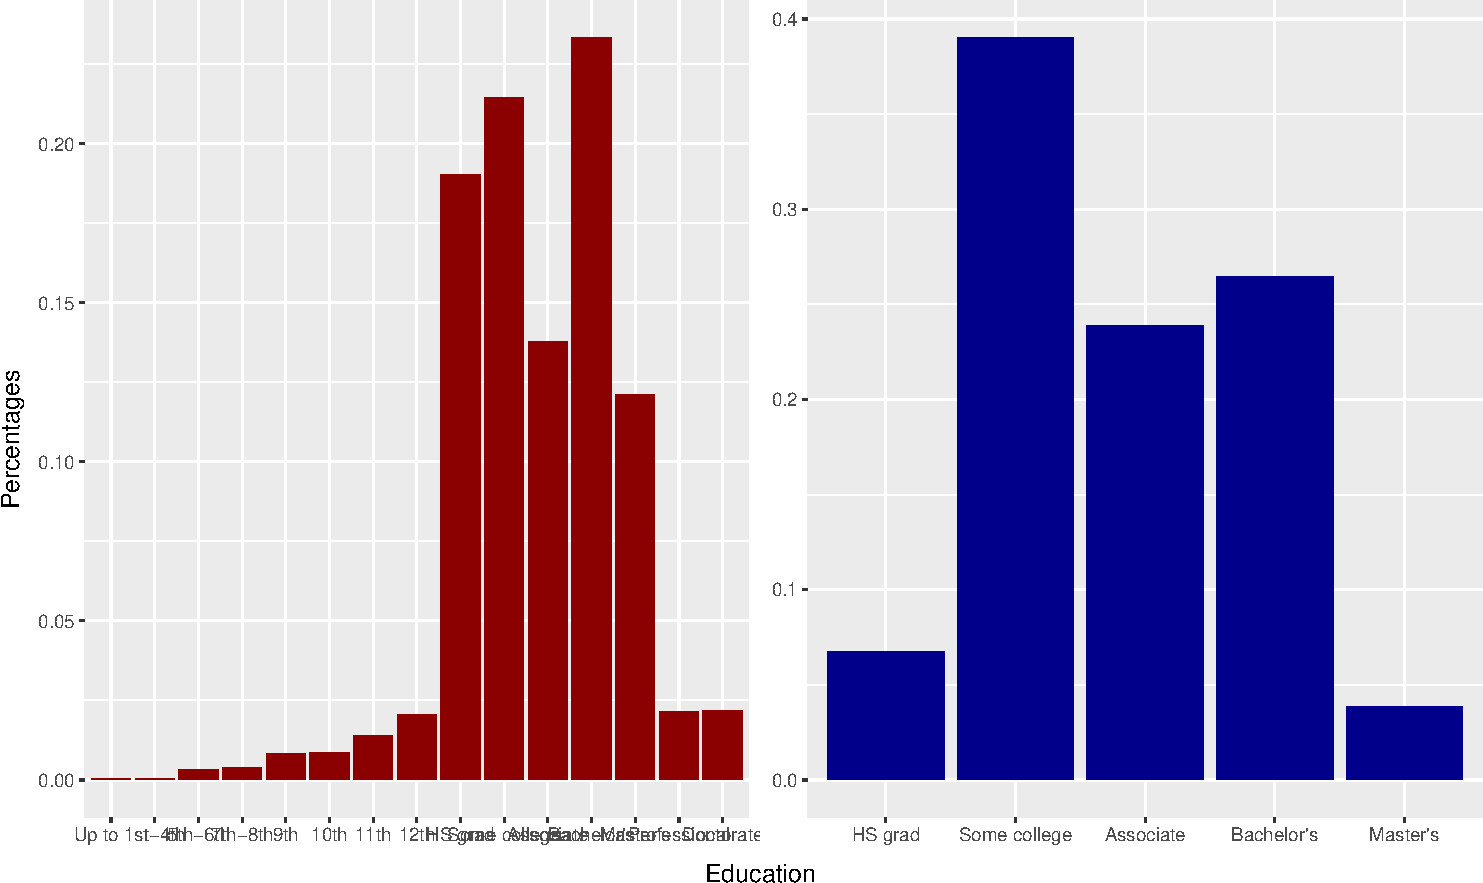
\includegraphics{dissertation_files/figure-latex/Barplot-Education-Categories-1.pdf}
\caption{\label{fig:Barplot-Education-Categories}Distribution of Education Categories. Original 2016 ANES categories on the left, ordered probit estimated categories on the right\label{BarEducCat}}
\end{figure}
As we can see, all categories `below' ``High school graduate'' and `above' ``Master's'' are collapsed because they do not fit the data. The ordered probit model uses the ordinal information with unevenly spaced distances provided and returns categories that do fit the data. We can now use these estimated education categories as the basis for blocking. Assigning numeric values to the new categories is now justifiable because they are based on data-driven estimations. This allows us to block on numerical values with the Mahalanobis distance, which would not be possible without empirical justification. The following sections show that the new estimated categories significantly affect analyses and results.

\hypertarget{ordblock-data-sims}{%
\subsection{Simulations}\label{ordblock-data-sims}}

I conduct various simulations to compare the Ordered Probit Model and its resulting reestimated education categories with the original ANES categories.

\hypertarget{ordblock-data-sims-plac}{%
\subsubsection{Placebo Regression}\label{ordblock-data-sims-plac}}

We separately block the 2016 ANES on the original and the ordered probit education categories into two treatment groups. We then model the following OLS regression on an interval response variable, a feeling thermometer towards Donald Trump as the Republican presidential candidate:

\vspace{-1cm}

\[Feel.Trump \sim Group + Dem + Rep + Income + Male + White + Black + Hispanic\]

\texttt{Group} indicates a placebo treatment, as no actual treatment is administered. In the absence of actual treatment, the difference between both treatment groups should thus be zero.

\hypertarget{ordblock-data-framing}{%
\subsection{Framing Survey}\label{ordblock-data-framing}}

\hypertarget{ordblock-results}{%
\section{Results}\label{ordblock-results}}

\hypertarget{ordblock-results-plac}{%
\subsection{Placebo Regression}\label{ordblock-results-plac}}

To test this, each blocking/regression process for each set of categories is repeated 1,000 times. The distribution of the placebo treatment indicator (\texttt{Group}) is visualized in Figure \ref{DensPlacTreat}.
\begin{figure}
\centering
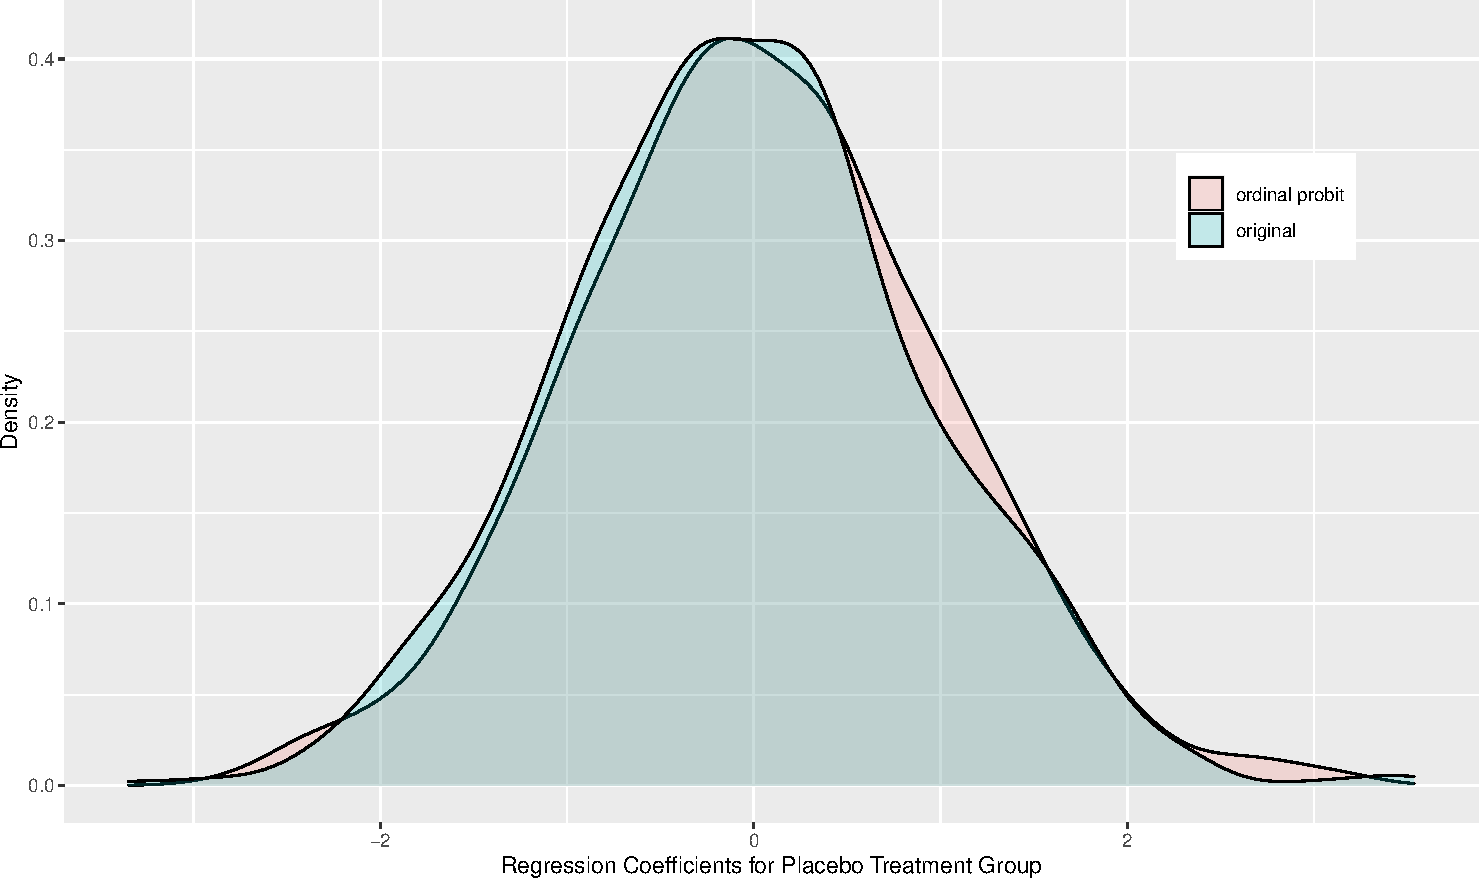
\includegraphics{dissertation_files/figure-latex/Density-Plot-Placebo-Treatment-1.pdf}
\caption{\label{fig:Density-Plot-Placebo-Treatment}Distribution of placebo treatment coefficients by education model\label{DensPlacTreat}}
\end{figure}
Both distributions center around zero, as is the statistical expectation. Upon closer inspection, the ordered probit categories are closer to the true values than the original categories on both mean (0.019 v. -0.05) and median (-0.01 v. -0.07). This indicates slightly superior performance by the ordered probit categories.

\hypertarget{ordblock-results-framing}{%
\subsection{Framing Survey}\label{ordblock-results-framing}}

Put text here

\hypertarget{ordmiss}{%
\chapter{QUALITY COMPARISON OF MAJOR MISSING DATA SOLUTIONS FOR DISCRETE DATA WITH A PROPOSED NEW METHOD FOR ORDINAL VARIABLES}\label{ordmiss}}

\hypertarget{ordmiss-intro}{%
\section{Introduction}\label{ordmiss-intro}}

Missing data are ubiquitous in survey research (Allison, 2002; Raghunathan, 2016). Respondents frequently refuse to answer questions, select ``Don't Know'' as a response option, or drop out during the response collection process (Honaker \& King, 2010). Missing data pose a big problem for researchers because data can typically not be analyzed with statistical software if they contain missing values (Little \& Rubin, 2002; Molenberghs \& Kenward, 2007).

Scholars have developed several general ways to treat missing data. These range from deleting all observations with missing data (listwise deletion) over randomly drawing a `similar' respondent to provide a fill-in value for a missing slot (hot decking) to estimating missing values from conditional distributions (multiple imputation) (Fay, 1996; King, Honaker, Joseph, \& Scheve, 2001; Rubin, 1976).

Listwise deletion has been shown to induce bias with political data (Rees \& Duke-Williams, 1997; Reilly, 1993). +++ more citations, examples of how widely used listwise deletion is

Hot decking does not reflect statistical uncertainty in the filled-in values since there is only one draw (Gill \& Witko, 2013; Kroh, 2006). +++ More detail about the method

Multiple implementation has become the state of the art in missing data management +++ citations, examples, reasons why it's the state of the art

However, multiple imputation is not necessarily always the most suitable method for all types of variables. For non-granular discrete data, for instance, multiple hot deck imputation, a variation over generic multiple imputation, proves more precise (Gill \& Cranmer, 2012). +++ how does it achieve that

However, multiple hot deck imputation assumes even distances between categories in discrete data. This assumption does not necessarily apply for ordinal variables. I propose a method designed to impute discrete missing data specifically from ordinal variables. Because of the success of multiple hot deck imputation, this method is based on multiple hot deck imputation and adapted to account for the specific circumstances of ordinal variables. Based on the ordered probit model approach in chapter II, it applies a weighted distance solution with newly estimated numeric thresholds from an assumed underlying latent continuous variable to measure the distances between the categories and calculate an affinity score.

This chapter will:

-- Provide theory behind missing data mechanisms, deletion, imputation, multiple imputation
-- Outline \texttt{R} packages/functions that implement listwise deletion and variations of multiple imputation, including my proposed new method
-- \texttt{na.omit()}
-- \texttt{amelia()}
-- \texttt{mice()}
-- \texttt{hot.deck()}
-- \texttt{hd.ord()}
-- Apply these \texttt{R} packages to three different sets of survey data
-- Test each package for accuracy and speed for differing types of variables
-- Assess the usefulness of my proposed new method

\hypertarget{ordmiss-theory}{%
\section{Theory}\label{ordmiss-theory}}

\hypertarget{ordmiss-theory-mechanisms}{%
\subsection{Missing Data Mechanisms}\label{ordmiss-theory-mechanisms}}

MCAR
MAR
NMAR

\hypertarget{ordmiss-theory-delete}{%
\subsection{Deletion}\label{ordmiss-theory-delete}}

Deletion of incomplete observations, listwise deletion

\hypertarget{ordmiss-theory-impute}{%
\subsection{Imputation}\label{ordmiss-theory-impute}}

\hypertarget{ordmiss-theory-impute-mean}{%
\subsubsection{Mean}\label{ordmiss-theory-impute-mean}}

Mean is used to substitute values

\hypertarget{ordmiss-theory-impute-regress}{%
\subsubsection{Regression}\label{ordmiss-theory-impute-regress}}

Missing variables for a unit are estimated by predicted values from the regression on the known variables for that unit

\hypertarget{ordmiss-theory-impute-hd}{%
\subsubsection{Hot Decking}\label{ordmiss-theory-impute-hd}}

Recorded units in the sample are used to substitute values

Hot decking (Marker, Juddkins, Winglee (2002), Ernst (198), Kalton and Kish (1981), Ford (1983), David et al.~(1986)) (chapter 4, (Little \& Rubin, 2002))
-- by simple random sampling with replacement
-- within adjustment cells
-- nearest neighbor
-- sequential ordered by a covariate

\texttt{R} package: +++

\hypertarget{ordmiss-theory-multimpute}{%
\subsection{Multiple Imputation}\label{ordmiss-theory-multimpute}}

\hypertarget{ordmiss-theory-multimpute-amelia}{%
\subsubsection{\texorpdfstring{\texttt{Amelia}}{Amelia}}\label{ordmiss-theory-multimpute-amelia}}

\hypertarget{ordmiss-theory-multimpute-mice}{%
\subsubsection{\texorpdfstring{\texttt{mice}}{mice}}\label{ordmiss-theory-multimpute-mice}}

\hypertarget{ordmiss-theory-multimpute-hdnorm}{%
\subsubsection{Multiple Hot Deck Imputation}\label{ordmiss-theory-multimpute-hdnorm}}

\texttt{R} package: \texttt{hot.deck}

Multiple hot deck imputation (all COPIED OVER from Cranmer, Gill):
-- A non-parametric alternative to multiple imputation
-- A variation of hot deck imputation combined with the repeated imputation and estimation method typical of parametric multiple imputation
-- Designed to work well in situations where (traditional) parametric multiple imputation falls short -- when a discrete variable with a small number of categories has missing values. This can produce nonsensical imputations, biased results and artificially smaller standard errors
-- Maintains the integrity of the data by using draws of actual values from the variable with the missing values to impute missing items
-- Maintains the discrete nature of discrete data and produces more accurate imputations than parametric multiple imputation in a majority of social science applications where the data are discrete
-- Since many political science applications rely on highly discrete measures, multiple hot deck imputation provides the researcher with more accuracy in imputations than parametric multiple imputation, while requiring none of parametric multiple imputation's standard assumptions

Concrete estimation steps:
(1) Create several copies of the dataset.
(2) Search down columns of the data sequentially looking for missing observations
a) When a missing value is found, compute a vector of affinity scores, for that missing value. This vector is as long as the number of rows in the dataset, minus any rows with missing values for the same variable
b) Create the imputation cell of best donors for this missing value and draw randomly from it to produce a vector of imputations
c) Impute one of these values into the appropriate cell of each duplicate dataset for this missing value
(3) Repeat Step 2 until no missing observations remain
(4) Fit the statistic of interest for each dataset
(5) Combine the estimates of the statistic into a single estimate using the combination rules of parametric multiple imputation

\hypertarget{ordmiss-theory-multimpute-hdord}{%
\subsubsection{Ordinal Variable Multiple Hot Deck Imputation}\label{ordmiss-theory-multimpute-hdord}}

Imputation techniques rely on continuous distributional assumptions.
I use my ordered probit estimated latent underlying continuous variable.

Ordinal hot deck imputation:
-- An extension of multiple hot deck imputation
-- Designed specifically to implement multiple hot deck imputation with ordinal variables
-- Fully utilizes the unevenly spaced yet ordered information provided in ordinal variables
-- A key variable in political science surveys is ordinal: Education. Ordinal hot deck imputation enables researchers to impute missing data using the full information provided in this most important predictor variable

Multiple hot deck imputation uses draws of values from the variable with the missing values (hot decking) to impute them distributionally (multiple imputation) and estimate affinity scores. This score measures how close other respondents are to the one with the missing value. `Closeness' is measured as the distance between respondents in the variables that do not contain missing values. This is best illustrated with simplified data shown in Table \ref{ordmiss-affscore}.
\begin{table}[ht]
  \centering
  \begin{tabular}{lccccc}
  \bottomrule 
  \midrule
  Respondent & Age & Party ID & Education & Income & Gender\\
  \hline
  A & 25 & Republican & High School Graduate & \$40-50,000 & Male \\
  B & 40 & NA & Some High School &  \$30-40,000 & Female\\
  C & 30 & Democrat & Bachelor's Degree &  \$60-70,000 & Female\\
  \bottomrule 
  \end{tabular}
  \caption{Illustrative Data}
  \label{ordmiss-affscore}
\end{table}
Respondent B shows missing data for party ID. To impute a fill-in value, we look at how close respondents A and C are to B in terms of age, education, income, and gender. C is closer to B in terms of age and they share the same gender. A is closer to B on education and income. Multiple hot deck imputation measures these distances and estimates affinity scores for respondents A and C. B then receives the party ID fill-in value from whichever respondent has the higher score. The algorithm building the affinity score, however, assumes evenly spaced distances between categories. This is the case for age, income, and gender, but not for education, since education is an ordinal variable. Applying multiple hot deck imputation here would misrepresent the data.

\texttt{R} functions: \texttt{hd.ord()}

\texttt{education} is crucial to test the performance of \texttt{hd.ord}, which was designed specifically for ordinal variables. \texttt{hd.ord} in turn depends on another specifically designed function called \texttt{OPMOrd}. \texttt{OPMOrd} applies \texttt{polr()} to an ordinal variable (here \texttt{education}) to estimate the underlying latent continuous variable. \texttt{polr()} can only be run on data without missing variables. +++

\hypertarget{ordmiss-data}{%
\section{Data}\label{ordmiss-data}}

I ampute data for three different sets of survey data: An experiment on moral framing I ran on MTurk in 2017 (original data), data from the 2016 ANES, and data from the 2016 CCES. All data are amputed with the \texttt{ampute()} function from the \texttt{mice} package (+++ some citation that talks about ampute here). Each data set is imputed with five different functions: \texttt{amelia()}, \texttt{mice()}, \texttt{hd.ord()}, \texttt{hot.deck()}, and \texttt{na.omit()}.

\texttt{amelia()} is from the \texttt{Amelia} package. \texttt{mice()} is from the \texttt{mice} package. Both are used with their default settings unless specified otherwise. \texttt{hot.deck()} is from Gill and Cranmer's multiple hot deck imputation package \texttt{hot.deck}. \texttt{hd.ord()} is my ordinal variable adaptation of \texttt{hot.deck()}. \texttt{na.omit()} applies list-wise deletion. I test each function for imputation accuracy and speed for binary, ordinal, and nominal variables in all three data sets. Each data set contains two ordinal (\texttt{Education}, \texttt{Interest}), two nominal (\texttt{Age}, \texttt{Income}) and numerous binary variables. In order to enable factually accurate comparison and unless specified otherwise, each data set contains 1,000 observations and six levels of the ordinal variable \texttt{Education}. 1,000 observations represent a common size for survey experiment data, and the \texttt{polr()} analysis from section \ref{ordblock-data} estimates five or six levels to best represent \texttt{Education} in a US context. Imputation of each data set was carried out with each of the five imputation methods for 1,000 iterations. With the exception of Table \ref{mar.5var.old.frame}, 20 percent NA were randomly amputed in each iteration for each data set.

Sections \ref{ordmiss-results-mar} to \ref{ordmiss-results-increaseNA} show the results in terms of performance accuracy. Since each data set is complete, we know the true variable mean of all variables. This serves as the baseline of comparison for the performance of each imputation method. First, I impute all data sets MAR (section \ref{ordmiss-results-mar}) and MNAR (section \ref{ordmiss-results-mnar}) for five and 12 amputed variables. The five amputed variables are consistent across all three data sets: \texttt{Democrat} (binary), \texttt{Male} (binary), \texttt{Interest} (ordinal), \texttt{Income} (nominal), and \texttt{Age} (nominal). The 12 amputed variables contain additional variables that differ between each data set due to availability in the data. In section \ref{ordmiss-results-increaseOrd}, I then increase the number of ordinal variables to be treated by \texttt{polr()} for \texttt{hd.ord()} by including \texttt{Interest}. Imputations also also conducted MAR and MNAR for four and 11 amputed variables. The variables are the same as in sections \ref{ordmiss-results-mar} and \ref{ordmiss-results-mnar}, but without including \texttt{Interest}. Finally, I increase the amount of missing data to 50 and 80 percent (section \ref{ordmiss-results-increaseNA}).

Section \ref{ordmiss-results-speed} shows the results in terms of performance speed by the number of imputed variables (Table \ref{runtimes5var12var}) and the percentage of missingness (Table \ref{run.all.perc}). All running times were achieved on a Code Ocean AWS EC2 instance with 16 cores and 120 GB of memory.

\hypertarget{ordmiss-results}{%
\section{Results}\label{ordmiss-results}}

\hypertarget{ordmiss-results-mar}{%
\subsection{MAR}\label{ordmiss-results-mar}}
\begin{table}[!htbp] \centering 
  \caption{Accuracy of Multiple Imputation Methods. MAR, 5 Variables with NA} 
  \label{mar.5var} 
\begin{threeparttable}
\begin{tabular}{@{\extracolsep{5pt}} D{.}{.}{-4} D{.}{.}{-4} D{.}{.}{-4} D{.}{.}{-4} D{.}{.}{-4} } 
\\[-1.8ex]\hline 
\hline \\[-1.8ex] 
\multicolumn{1}{c}{Method} & \multicolumn{1}{c}{Variable} & \multicolumn{1}{c}{ANES} & \multicolumn{1}{c}{CCES} & \multicolumn{1}{c}{Framing} \\ 
\hline \\[-1.8ex] 
\multicolumn{1}{c}{true} & \multicolumn{1}{c}{Dem} & \multicolumn{1}{c}{.3420} & \multicolumn{1}{c}{.3770} & \multicolumn{1}{c}{.4660} \\ 
\multicolumn{1}{c}{hot.deck} & \multicolumn{1}{c}{Dem} & \multicolumn{1}{c}{--.0010} & \multicolumn{1}{c}{+.0000} & \multicolumn{1}{c}{+.0001} \\ 
\multicolumn{1}{c}{hd.ord} & \multicolumn{1}{c}{Dem} & \multicolumn{1}{c}{--.0011} & \multicolumn{1}{c}{--.0004} & \multicolumn{1}{c}{+.0008} \\ 
\multicolumn{1}{c}{amelia} & \multicolumn{1}{c}{Dem} & \multicolumn{1}{c}{+.0004} & \multicolumn{1}{c}{+.0001} & \multicolumn{1}{c}{--.0001} \\ 
\multicolumn{1}{c}{mice} & \multicolumn{1}{c}{Dem} & \multicolumn{1}{c}{+.0003} & \multicolumn{1}{c}{+.0002} & \multicolumn{1}{c}{+.0000} \\ 
\multicolumn{1}{c}{na.omit} & \multicolumn{1}{c}{Dem} & \multicolumn{1}{c}{--.0290} & \multicolumn{1}{c}{--.0229} & \multicolumn{1}{c}{--.0340} \\ 
\multicolumn{1}{c}{true} & \multicolumn{1}{c}{Male} & \multicolumn{1}{c}{.4890} & \multicolumn{1}{c}{.4830} & \multicolumn{1}{c}{.5260} \\ 
\multicolumn{1}{c}{hot.deck} & \multicolumn{1}{c}{Male} & \multicolumn{1}{c}{--.0013} & \multicolumn{1}{c}{--.0011} & \multicolumn{1}{c}{+.0001} \\ 
\multicolumn{1}{c}{hd.ord} & \multicolumn{1}{c}{Male} & \multicolumn{1}{c}{--.0013} & \multicolumn{1}{c}{--.0014} & \multicolumn{1}{c}{+.0005} \\ 
\multicolumn{1}{c}{amelia} & \multicolumn{1}{c}{Male} & \multicolumn{1}{c}{+.0002} & \multicolumn{1}{c}{--.0001} & \multicolumn{1}{c}{+.0000} \\ 
\multicolumn{1}{c}{mice} & \multicolumn{1}{c}{Male} & \multicolumn{1}{c}{+.0001} & \multicolumn{1}{c}{--.0001} & \multicolumn{1}{c}{--.0001} \\ 
\multicolumn{1}{c}{na.omit} & \multicolumn{1}{c}{Male} & \multicolumn{1}{c}{--.0392} & \multicolumn{1}{c}{--.0414} & \multicolumn{1}{c}{--.0256} \\ 
\multicolumn{1}{c}{true} & \multicolumn{1}{c}{Interest} & \multicolumn{1}{c}{2.9340} & \multicolumn{1}{c}{3.3290} & \multicolumn{1}{c}{3.2170} \\ 
\multicolumn{1}{c}{hot.deck} & \multicolumn{1}{c}{Interest} & \multicolumn{1}{c}{--.0130} & \multicolumn{1}{c}{--.0125} & \multicolumn{1}{c}{--.0213} \\ 
\multicolumn{1}{c}{hd.ord} & \multicolumn{1}{c}{Interest} & \multicolumn{1}{c}{--.0191} & \multicolumn{1}{c}{--.0196} & \multicolumn{1}{c}{--.0248} \\ 
\multicolumn{1}{c}{amelia} & \multicolumn{1}{c}{Interest} & \multicolumn{1}{c}{+.0003} & \multicolumn{1}{c}{+.0003} & \multicolumn{1}{c}{--.0002} \\ 
\multicolumn{1}{c}{mice} & \multicolumn{1}{c}{Interest} & \multicolumn{1}{c}{+.0003} & \multicolumn{1}{c}{+.0000} & \multicolumn{1}{c}{--.0003} \\ 
\multicolumn{1}{c}{na.omit} & \multicolumn{1}{c}{Interest} & \multicolumn{1}{c}{--.0705} & \multicolumn{1}{c}{--.0724} & \multicolumn{1}{c}{--.0714} \\ 
\multicolumn{1}{c}{true} & \multicolumn{1}{c}{Inc} & \multicolumn{1}{c}{16.6140} & \multicolumn{1}{c}{6.4810} & \multicolumn{1}{c}{3.0890} \\ 
\multicolumn{1}{c}{hot.deck} & \multicolumn{1}{c}{Inc} & \multicolumn{1}{c}{--.1068} & \multicolumn{1}{c}{--.0259} & \multicolumn{1}{c}{--.0119} \\ 
\multicolumn{1}{c}{hd.ord} & \multicolumn{1}{c}{Inc} & \multicolumn{1}{c}{--.1278} & \multicolumn{1}{c}{--.0407} & \multicolumn{1}{c}{--.0192} \\ 
\multicolumn{1}{c}{amelia} & \multicolumn{1}{c}{Inc} & \multicolumn{1}{c}{+.0008} & \multicolumn{1}{c}{--.0004} & \multicolumn{1}{c}{+.0003} \\ 
\multicolumn{1}{c}{mice} & \multicolumn{1}{c}{Inc} & \multicolumn{1}{c}{+.0003} & \multicolumn{1}{c}{--.0002} & \multicolumn{1}{c}{+.0014} \\ 
\multicolumn{1}{c}{na.omit} & \multicolumn{1}{c}{Inc} & \multicolumn{1}{c}{--.5631} & \multicolumn{1}{c}{--.2468} & \multicolumn{1}{c}{--.1367} \\ 
\multicolumn{1}{c}{true} & \multicolumn{1}{c}{Age} & \multicolumn{1}{c}{50.0410} & \multicolumn{1}{c}{52.8230} & \multicolumn{1}{c}{37.9120} \\ 
\multicolumn{1}{c}{hot.deck} & \multicolumn{1}{c}{Age} & \multicolumn{1}{c}{--.3888} & \multicolumn{1}{c}{--.2616} & \multicolumn{1}{c}{--.3650} \\ 
\multicolumn{1}{c}{hd.ord} & \multicolumn{1}{c}{Age} & \multicolumn{1}{c}{--.4597} & \multicolumn{1}{c}{--.3895} & \multicolumn{1}{c}{--.3923} \\ 
\multicolumn{1}{c}{amelia} & \multicolumn{1}{c}{Age} & \multicolumn{1}{c}{+.0007} & \multicolumn{1}{c}{--.0033} & \multicolumn{1}{c}{--.0039} \\ 
\multicolumn{1}{c}{mice} & \multicolumn{1}{c}{Age} & \multicolumn{1}{c}{+.0017} & \multicolumn{1}{c}{--.0073} & \multicolumn{1}{c}{--.0049} \\ 
\multicolumn{1}{c}{na.omit} & \multicolumn{1}{c}{Age} & \multicolumn{1}{c}{--1.1875} & \multicolumn{1}{c}{--1.2361} & \multicolumn{1}{c}{--1.0641} \\
\hline \\[-1.8ex] 
\end{tabular} 
\begin{tablenotes}[para,flushleft]
\footnotesize{\textit{Note:} Each \texttt{true} value shows the true variable mean. All other values show the differences between the imputation means and the true mean.}
\end{tablenotes}
\end{threeparttable}
\end{table}
\clearpage

\ssp

\footnotesize
\begin{longtable}{@{\extracolsep{5pt}} D{.}{.}{-4} D{.}{.}{-4} D{.}{.}{-4} D{.}{.}{-4} D{.}{.}{-4} } 
  \caption{Accuracy of Multiple Imputation Methods. MAR, 12 Variables with NA} 
  \label{mar.12var} 
\\[-1.8ex]\hline 
\hline \\[-1.8ex] 
\multicolumn{1}{c}{Method} & \multicolumn{1}{c}{Variable} & \multicolumn{1}{c}{ANES} & \multicolumn{1}{c}{CCES} & \multicolumn{1}{c}{Framing} \\ 
\hline \\[-1.8ex] 
\multicolumn{1}{c}{true} & \multicolumn{1}{c}{Dem} & \multicolumn{1}{c}{.3420} & \multicolumn{1}{c}{.3770} & \multicolumn{1}{c}{.4660} \\ 
\multicolumn{1}{c}{hot.deck} & \multicolumn{1}{c}{Dem} & \multicolumn{1}{c}{--.0005} & \multicolumn{1}{c}{--.0003} & \multicolumn{1}{c}{+.0001} \\ 
\multicolumn{1}{c}{hd.ord} & \multicolumn{1}{c}{Dem} & \multicolumn{1}{c}{--.0005} & \multicolumn{1}{c}{--.0004} & \multicolumn{1}{c}{+.0004} \\ 
\multicolumn{1}{c}{amelia} & \multicolumn{1}{c}{Dem} & \multicolumn{1}{c}{+.0000} & \multicolumn{1}{c}{+.0000} & \multicolumn{1}{c}{+.0001} \\ 
\multicolumn{1}{c}{mice} & \multicolumn{1}{c}{Dem} & \multicolumn{1}{c}{+.0000} & \multicolumn{1}{c}{+.0001} & \multicolumn{1}{c}{+.0001} \\ 
\multicolumn{1}{c}{na.omit} & \multicolumn{1}{c}{Dem} & \multicolumn{1}{c}{--.0191} & \multicolumn{1}{c}{--.0172} & \multicolumn{1}{c}{--.0280} \\ 
\multicolumn{1}{c}{true} & \multicolumn{1}{c}{Male} & \multicolumn{1}{c}{.4890} & \multicolumn{1}{c}{.4830} & \multicolumn{1}{c}{.5260} \\ 
\multicolumn{1}{c}{hot.deck} & \multicolumn{1}{c}{Male} & \multicolumn{1}{c}{--.0004} & \multicolumn{1}{c}{--.0002} & \multicolumn{1}{c}{--.0002} \\ 
\multicolumn{1}{c}{hd.ord} & \multicolumn{1}{c}{Male} & \multicolumn{1}{c}{--.0001} & \multicolumn{1}{c}{--.0003} & \multicolumn{1}{c}{+.0000} \\ 
\multicolumn{1}{c}{amelia} & \multicolumn{1}{c}{Male} & \multicolumn{1}{c}{+.0001} & \multicolumn{1}{c}{--.0001} & \multicolumn{1}{c}{--.0001} \\ 
\multicolumn{1}{c}{mice} & \multicolumn{1}{c}{Male} & \multicolumn{1}{c}{+.0000} & \multicolumn{1}{c}{--.0002} & \multicolumn{1}{c}{--.0001} \\ 
\multicolumn{1}{c}{na.omit} & \multicolumn{1}{c}{Male} & \multicolumn{1}{c}{--.0256} & \multicolumn{1}{c}{--.0364} & \multicolumn{1}{c}{--.0154} \\ 
\multicolumn{1}{c}{true} & \multicolumn{1}{c}{Interest} & \multicolumn{1}{c}{2.9340} & \multicolumn{1}{c}{3.3290} & \multicolumn{1}{c}{3.2170} \\ 
\multicolumn{1}{c}{hot.deck} & \multicolumn{1}{c}{Interest} & \multicolumn{1}{c}{--.0053} & \multicolumn{1}{c}{--.0041} & \multicolumn{1}{c}{--.0095} \\ 
\multicolumn{1}{c}{hd.ord} & \multicolumn{1}{c}{Interest} & \multicolumn{1}{c}{--.0077} & \multicolumn{1}{c}{--.0067} & \multicolumn{1}{c}{--.0106} \\ 
\multicolumn{1}{c}{amelia} & \multicolumn{1}{c}{Interest} & \multicolumn{1}{c}{+.0001} & \multicolumn{1}{c}{--.0001} & \multicolumn{1}{c}{+.0002} \\ 
\multicolumn{1}{c}{mice} & \multicolumn{1}{c}{Interest} & \multicolumn{1}{c}{+.0000} & \multicolumn{1}{c}{--.0001} & \multicolumn{1}{c}{--.0001} \\ 
\multicolumn{1}{c}{na.omit} & \multicolumn{1}{c}{Interest} & \multicolumn{1}{c}{--.0620} & \multicolumn{1}{c}{--.0515} & \multicolumn{1}{c}{--.0721} \\ 
\multicolumn{1}{c}{true} & \multicolumn{1}{c}{Inc} & \multicolumn{1}{c}{16.6140} & \multicolumn{1}{c}{6.4810} & \multicolumn{1}{c}{3.0890} \\ 
\multicolumn{1}{c}{hot.deck} & \multicolumn{1}{c}{Inc} & \multicolumn{1}{c}{--.0470} & \multicolumn{1}{c}{--.0130} & \multicolumn{1}{c}{--.0060} \\ 
\multicolumn{1}{c}{hd.ord} & \multicolumn{1}{c}{Inc} & \multicolumn{1}{c}{--.0591} & \multicolumn{1}{c}{--.0212} & \multicolumn{1}{c}{--.0089} \\ 
\multicolumn{1}{c}{amelia} & \multicolumn{1}{c}{Inc} & \multicolumn{1}{c}{--.0007} & \multicolumn{1}{c}{--.0005} & \multicolumn{1}{c}{--.0002} \\ 
\multicolumn{1}{c}{mice} & \multicolumn{1}{c}{Inc} & \multicolumn{1}{c}{--.0013} & \multicolumn{1}{c}{--.0003} & \multicolumn{1}{c}{+.0000} \\ 
\multicolumn{1}{c}{na.omit} & \multicolumn{1}{c}{Inc} & \multicolumn{1}{c}{--.6303} & \multicolumn{1}{c}{--.2860} & \multicolumn{1}{c}{--.0960} \\ 
\multicolumn{1}{c}{true} & \multicolumn{1}{c}{Age} & \multicolumn{1}{c}{50.0410} & \multicolumn{1}{c}{52.8230} & \multicolumn{1}{c}{37.9120} \\ 
\multicolumn{1}{c}{hot.deck} & \multicolumn{1}{c}{Age} & \multicolumn{1}{c}{--.1391} & \multicolumn{1}{c}{--.0883} & \multicolumn{1}{c}{--.1494} \\ 
\multicolumn{1}{c}{hd.ord} & \multicolumn{1}{c}{Age} & \multicolumn{1}{c}{--.1835} & \multicolumn{1}{c}{--.1435} & \multicolumn{1}{c}{--.1592} \\ 
\multicolumn{1}{c}{amelia} & \multicolumn{1}{c}{Age} & \multicolumn{1}{c}{+.0056} & \multicolumn{1}{c}{--.0015} & \multicolumn{1}{c}{--.0041} \\ 
\multicolumn{1}{c}{mice} & \multicolumn{1}{c}{Age} & \multicolumn{1}{c}{+.0048} & \multicolumn{1}{c}{--.0050} & \multicolumn{1}{c}{--.0029} \\ 
\multicolumn{1}{c}{na.omit} & \multicolumn{1}{c}{Age} & \multicolumn{1}{c}{--.8638} & \multicolumn{1}{c}{--.5974} & \multicolumn{1}{c}{--.6434} \\ 
\multicolumn{1}{c}{true} & \multicolumn{1}{c}{Black} & \multicolumn{1}{c}{.0790} & \multicolumn{1}{c}{.0950} & \multicolumn{1}{c}{.0690} \\ 
\multicolumn{1}{c}{hot.deck} & \multicolumn{1}{c}{Black} & \multicolumn{1}{c}{+.0000} & \multicolumn{1}{c}{+.0000} & \multicolumn{1}{c}{--.0001} \\ 
\multicolumn{1}{c}{hd.ord} & \multicolumn{1}{c}{Black} & \multicolumn{1}{c}{+.0000} & \multicolumn{1}{c}{+.0000} & \multicolumn{1}{c}{--.0003} \\ 
\multicolumn{1}{c}{amelia} & \multicolumn{1}{c}{Black} & \multicolumn{1}{c}{+.0000} & \multicolumn{1}{c}{+.0001} & \multicolumn{1}{c}{+.0000} \\ 
\multicolumn{1}{c}{mice} & \multicolumn{1}{c}{Black} & \multicolumn{1}{c}{+.0000} & \multicolumn{1}{c}{+.0001} & \multicolumn{1}{c}{+.0001} \\ 
\multicolumn{1}{c}{na.omit} & \multicolumn{1}{c}{Black} & \multicolumn{1}{c}{--.0092} & \multicolumn{1}{c}{--.0090} & \multicolumn{1}{c}{--.0110} \\ 
\multicolumn{1}{c}{true} & \multicolumn{1}{c}{Empl} & \multicolumn{1}{c}{.6610} & \multicolumn{1}{c}{.4370} & \multicolumn{1}{c}{.7430} \\ 
\multicolumn{1}{c}{hot.deck} & \multicolumn{1}{c}{Empl} & \multicolumn{1}{c}{+.0006} & \multicolumn{1}{c}{+.0000} & \multicolumn{1}{c}{+.0007} \\ 
\multicolumn{1}{c}{hd.ord} & \multicolumn{1}{c}{Empl} & \multicolumn{1}{c}{+.0006} & \multicolumn{1}{c}{+.0001} & \multicolumn{1}{c}{+.0006} \\ 
\multicolumn{1}{c}{amelia} & \multicolumn{1}{c}{Empl} & \multicolumn{1}{c}{+.0000} & \multicolumn{1}{c}{+.0000} & \multicolumn{1}{c}{+.0000} \\ 
\multicolumn{1}{c}{mice} & \multicolumn{1}{c}{Empl} & \multicolumn{1}{c}{+.0000} & \multicolumn{1}{c}{--.0001} & \multicolumn{1}{c}{--.0001} \\ 
\multicolumn{1}{c}{na.omit} & \multicolumn{1}{c}{Empl} & \multicolumn{1}{c}{--.0087} & \multicolumn{1}{c}{--.0301} & \multicolumn{1}{c}{--.0157} \\ 
\multicolumn{1}{c}{true} & \multicolumn{1}{c}{Religious} & \multicolumn{1}{c}{.6460} & \multicolumn{1}{c}{.6420} & \multicolumn{1}{c}{---} \\ 
\multicolumn{1}{c}{hot.deck} & \multicolumn{1}{c}{Religious} & \multicolumn{1}{c}{--.0006} & \multicolumn{1}{c}{--.0003} & \multicolumn{1}{c}{---} \\ 
\multicolumn{1}{c}{hd.ord} & \multicolumn{1}{c}{Religious} & \multicolumn{1}{c}{--.0005} & \multicolumn{1}{c}{--.0003} & \multicolumn{1}{c}{---} \\ 
\multicolumn{1}{c}{amelia} & \multicolumn{1}{c}{Religious} & \multicolumn{1}{c}{--.0001} & \multicolumn{1}{c}{--.0001} & \multicolumn{1}{c}{---} \\ 
\multicolumn{1}{c}{mice} & \multicolumn{1}{c}{Religious} & \multicolumn{1}{c}{--.0001} & \multicolumn{1}{c}{--.0002} & \multicolumn{1}{c}{---} \\ 
\multicolumn{1}{c}{na.omit} & \multicolumn{1}{c}{Religious} & \multicolumn{1}{c}{--.0166} & \multicolumn{1}{c}{--.0234} & \multicolumn{1}{c}{---} \\ 
\multicolumn{1}{c}{true} & \multicolumn{1}{c}{Married} & \multicolumn{1}{c}{.5290} & \multicolumn{1}{c}{.6310} & \multicolumn{1}{c}{---} \\ 
\multicolumn{1}{c}{hot.deck} & \multicolumn{1}{c}{Married} & \multicolumn{1}{c}{+.0002} & \multicolumn{1}{c}{--.0001} & \multicolumn{1}{c}{---} \\ 
\multicolumn{1}{c}{hd.ord} & \multicolumn{1}{c}{Married} & \multicolumn{1}{c}{+.0002} & \multicolumn{1}{c}{+.0001} & \multicolumn{1}{c}{---} \\ 
\multicolumn{1}{c}{amelia} & \multicolumn{1}{c}{Married} & \multicolumn{1}{c}{--.0001} & \multicolumn{1}{c}{--.0002} & \multicolumn{1}{c}{---} \\ 
\multicolumn{1}{c}{mice} & \multicolumn{1}{c}{Married} & \multicolumn{1}{c}{--.0001} & \multicolumn{1}{c}{--.0002} & \multicolumn{1}{c}{---} \\ 
\multicolumn{1}{c}{na.omit} & \multicolumn{1}{c}{Married} & \multicolumn{1}{c}{--.0384} & \multicolumn{1}{c}{--.0326} & \multicolumn{1}{c}{---} \\ 
\multicolumn{1}{c}{true} & \multicolumn{1}{c}{OwnHome} & \multicolumn{1}{c}{.6820} & \multicolumn{1}{c}{.7010} & \multicolumn{1}{c}{---} \\ 
\multicolumn{1}{c}{hot.deck} & \multicolumn{1}{c}{OwnHome} & \multicolumn{1}{c}{--.0001} & \multicolumn{1}{c}{--.0002} & \multicolumn{1}{c}{---} \\ 
\multicolumn{1}{c}{hd.ord} & \multicolumn{1}{c}{OwnHome} & \multicolumn{1}{c}{+.0000} & \multicolumn{1}{c}{+.0000} & \multicolumn{1}{c}{---} \\ 
\multicolumn{1}{c}{amelia} & \multicolumn{1}{c}{OwnHome} & \multicolumn{1}{c}{+.0001} & \multicolumn{1}{c}{+.0000} & \multicolumn{1}{c}{---} \\ 
\multicolumn{1}{c}{mice} & \multicolumn{1}{c}{OwnHome} & \multicolumn{1}{c}{--.0001} & \multicolumn{1}{c}{--.0001} & \multicolumn{1}{c}{---} \\ 
\multicolumn{1}{c}{na.omit} & \multicolumn{1}{c}{OwnHome} & \multicolumn{1}{c}{--.0334} & \multicolumn{1}{c}{--.0304} & \multicolumn{1}{c}{---} \\ 
\multicolumn{1}{c}{true} & \multicolumn{1}{c}{Rally} & \multicolumn{1}{c}{.0830} & \multicolumn{1}{c}{---} & \multicolumn{1}{c}{---} \\ 
\multicolumn{1}{c}{hot.deck} & \multicolumn{1}{c}{Rally} & \multicolumn{1}{c}{--.0001} & \multicolumn{1}{c}{---} & \multicolumn{1}{c}{---} \\ 
\multicolumn{1}{c}{hd.ord} & \multicolumn{1}{c}{Rally} & \multicolumn{1}{c}{--.0002} & \multicolumn{1}{c}{---} & \multicolumn{1}{c}{---} \\ 
\multicolumn{1}{c}{amelia} & \multicolumn{1}{c}{Rally} & \multicolumn{1}{c}{+.0001} & \multicolumn{1}{c}{---} & \multicolumn{1}{c}{---} \\ 
\multicolumn{1}{c}{mice} & \multicolumn{1}{c}{Rally} & \multicolumn{1}{c}{+.0001} & \multicolumn{1}{c}{---} & \multicolumn{1}{c}{---} \\ 
\multicolumn{1}{c}{na.omit} & \multicolumn{1}{c}{Rally} & \multicolumn{1}{c}{--.0191} & \multicolumn{1}{c}{---} & \multicolumn{1}{c}{---} \\ 
\multicolumn{1}{c}{true} & \multicolumn{1}{c}{Donate} & \multicolumn{1}{c}{.1390} & \multicolumn{1}{c}{---} & \multicolumn{1}{c}{---} \\ 
\multicolumn{1}{c}{hot.deck} & \multicolumn{1}{c}{Donate} & \multicolumn{1}{c}{--.0002} & \multicolumn{1}{c}{---} & \multicolumn{1}{c}{---} \\ 
\multicolumn{1}{c}{hd.ord} & \multicolumn{1}{c}{Donate} & \multicolumn{1}{c}{--.0005} & \multicolumn{1}{c}{---} & \multicolumn{1}{c}{---} \\ 
\multicolumn{1}{c}{amelia} & \multicolumn{1}{c}{Donate} & \multicolumn{1}{c}{+.0000} & \multicolumn{1}{c}{---} & \multicolumn{1}{c}{---} \\ 
\multicolumn{1}{c}{mice} & \multicolumn{1}{c}{Donate} & \multicolumn{1}{c}{+.0001} & \multicolumn{1}{c}{---} & \multicolumn{1}{c}{---} \\ 
\multicolumn{1}{c}{na.omit} & \multicolumn{1}{c}{Donate} & \multicolumn{1}{c}{--.0320} & \multicolumn{1}{c}{---} & \multicolumn{1}{c}{---} \\ 
\multicolumn{1}{c}{true} & \multicolumn{1}{c}{Gay} & \multicolumn{1}{c}{---} & \multicolumn{1}{c}{.0420} & \multicolumn{1}{c}{---} \\ 
\multicolumn{1}{c}{hot.deck} & \multicolumn{1}{c}{Gay} & \multicolumn{1}{c}{---} & \multicolumn{1}{c}{+.0001} & \multicolumn{1}{c}{---} \\ 
\multicolumn{1}{c}{hd.ord} & \multicolumn{1}{c}{Gay} & \multicolumn{1}{c}{---} & \multicolumn{1}{c}{+.0000} & \multicolumn{1}{c}{---} \\ 
\multicolumn{1}{c}{amelia} & \multicolumn{1}{c}{Gay} & \multicolumn{1}{c}{---} & \multicolumn{1}{c}{+.0000} & \multicolumn{1}{c}{---} \\ 
\multicolumn{1}{c}{mice} & \multicolumn{1}{c}{Gay} & \multicolumn{1}{c}{---} & \multicolumn{1}{c}{+.0000} & \multicolumn{1}{c}{---} \\ 
\multicolumn{1}{c}{na.omit} & \multicolumn{1}{c}{Gay} & \multicolumn{1}{c}{---} & \multicolumn{1}{c}{--.0112} & \multicolumn{1}{c}{---} \\ 
\multicolumn{1}{c}{true} & \multicolumn{1}{c}{StudLoans} & \multicolumn{1}{c}{---} & \multicolumn{1}{c}{.1910} & \multicolumn{1}{c}{---} \\ 
\multicolumn{1}{c}{hot.deck} & \multicolumn{1}{c}{StudLoans} & \multicolumn{1}{c}{---} & \multicolumn{1}{c}{+.0003} & \multicolumn{1}{c}{---} \\ 
\multicolumn{1}{c}{hd.ord} & \multicolumn{1}{c}{StudLoans} & \multicolumn{1}{c}{---} & \multicolumn{1}{c}{+.0002} & \multicolumn{1}{c}{---} \\ 
\multicolumn{1}{c}{amelia} & \multicolumn{1}{c}{StudLoans} & \multicolumn{1}{c}{---} & \multicolumn{1}{c}{+.0000} & \multicolumn{1}{c}{---} \\ 
\multicolumn{1}{c}{mice} & \multicolumn{1}{c}{StudLoans} & \multicolumn{1}{c}{---} & \multicolumn{1}{c}{--.0001} & \multicolumn{1}{c}{---} \\ 
\multicolumn{1}{c}{na.omit} & \multicolumn{1}{c}{StudLoans} & \multicolumn{1}{c}{---} & \multicolumn{1}{c}{--.0117} & \multicolumn{1}{c}{---} \\ 
\multicolumn{1}{c}{true} & \multicolumn{1}{c}{Hisp} & \multicolumn{1}{c}{---} & \multicolumn{1}{c}{---} & \multicolumn{1}{c}{.0550} \\ 
\multicolumn{1}{c}{hot.deck} & \multicolumn{1}{c}{Hisp} & \multicolumn{1}{c}{---} & \multicolumn{1}{c}{---} & \multicolumn{1}{c}{--.0002} \\ 
\multicolumn{1}{c}{hd.ord} & \multicolumn{1}{c}{Hisp} & \multicolumn{1}{c}{---} & \multicolumn{1}{c}{---} & \multicolumn{1}{c}{--.0002} \\ 
\multicolumn{1}{c}{amelia} & \multicolumn{1}{c}{Hisp} & \multicolumn{1}{c}{---} & \multicolumn{1}{c}{---} & \multicolumn{1}{c}{+.0000} \\ 
\multicolumn{1}{c}{mice} & \multicolumn{1}{c}{Hisp} & \multicolumn{1}{c}{---} & \multicolumn{1}{c}{---} & \multicolumn{1}{c}{+.0000} \\ 
\multicolumn{1}{c}{na.omit} & \multicolumn{1}{c}{Hisp} & \multicolumn{1}{c}{---} & \multicolumn{1}{c}{---} & \multicolumn{1}{c}{--.0072} \\ 
\multicolumn{1}{c}{true} & \multicolumn{1}{c}{Official} & \multicolumn{1}{c}{---} & \multicolumn{1}{c}{---} & \multicolumn{1}{c}{.3560} \\ 
\multicolumn{1}{c}{hot.deck} & \multicolumn{1}{c}{Official} & \multicolumn{1}{c}{---} & \multicolumn{1}{c}{---} & \multicolumn{1}{c}{+.0000} \\ 
\multicolumn{1}{c}{hd.ord} & \multicolumn{1}{c}{Official} & \multicolumn{1}{c}{---} & \multicolumn{1}{c}{---} & \multicolumn{1}{c}{--.0003} \\ 
\multicolumn{1}{c}{amelia} & \multicolumn{1}{c}{Official} & \multicolumn{1}{c}{---} & \multicolumn{1}{c}{---} & \multicolumn{1}{c}{+.0001} \\ 
\multicolumn{1}{c}{mice} & \multicolumn{1}{c}{Official} & \multicolumn{1}{c}{---} & \multicolumn{1}{c}{---} & \multicolumn{1}{c}{+.0001} \\ 
\multicolumn{1}{c}{na.omit} & \multicolumn{1}{c}{Official} & \multicolumn{1}{c}{---} & \multicolumn{1}{c}{---} & \multicolumn{1}{c}{--.0385} \\ 
\multicolumn{1}{c}{true} & \multicolumn{1}{c}{Stud} & \multicolumn{1}{c}{---} & \multicolumn{1}{c}{---} & \multicolumn{1}{c}{.0440} \\ 
\multicolumn{1}{c}{hot.deck} & \multicolumn{1}{c}{Stud} & \multicolumn{1}{c}{---} & \multicolumn{1}{c}{---} & \multicolumn{1}{c}{+.0000} \\ 
\multicolumn{1}{c}{hd.ord} & \multicolumn{1}{c}{Stud} & \multicolumn{1}{c}{---} & \multicolumn{1}{c}{---} & \multicolumn{1}{c}{+.0000} \\ 
\multicolumn{1}{c}{amelia} & \multicolumn{1}{c}{Stud} & \multicolumn{1}{c}{---} & \multicolumn{1}{c}{---} & \multicolumn{1}{c}{+.0000} \\ 
\multicolumn{1}{c}{mice} & \multicolumn{1}{c}{Stud} & \multicolumn{1}{c}{---} & \multicolumn{1}{c}{---} & \multicolumn{1}{c}{+.0001} \\ 
\multicolumn{1}{c}{na.omit} & \multicolumn{1}{c}{Stud} & \multicolumn{1}{c}{---} & \multicolumn{1}{c}{---} & \multicolumn{1}{c}{--.0012} \\ 
\multicolumn{1}{c}{true} & \multicolumn{1}{c}{Media} & \multicolumn{1}{c}{---} & \multicolumn{1}{c}{---} & \multicolumn{1}{c}{1.7240} \\ 
\multicolumn{1}{c}{hot.deck} & \multicolumn{1}{c}{Media} & \multicolumn{1}{c}{---} & \multicolumn{1}{c}{---} & \multicolumn{1}{c}{--.0049} \\ 
\multicolumn{1}{c}{hd.ord} & \multicolumn{1}{c}{Media} & \multicolumn{1}{c}{---} & \multicolumn{1}{c}{---} & \multicolumn{1}{c}{--.0060} \\ 
\multicolumn{1}{c}{amelia} & \multicolumn{1}{c}{Media} & \multicolumn{1}{c}{---} & \multicolumn{1}{c}{---} & \multicolumn{1}{c}{+.0001} \\ 
\multicolumn{1}{c}{mice} & \multicolumn{1}{c}{Media} & \multicolumn{1}{c}{---} & \multicolumn{1}{c}{---} & \multicolumn{1}{c}{+.0001} \\ 
\multicolumn{1}{c}{na.omit} & \multicolumn{1}{c}{Media} & \multicolumn{1}{c}{---} & \multicolumn{1}{c}{---} & \multicolumn{1}{c}{--.0984} \\ 
\multicolumn{1}{c}{true} & \multicolumn{1}{c}{Participation} & \multicolumn{1}{c}{---} & \multicolumn{1}{c}{---} & \multicolumn{1}{c}{.9540} \\ 
\multicolumn{1}{c}{hot.deck} & \multicolumn{1}{c}{Participation} & \multicolumn{1}{c}{---} & \multicolumn{1}{c}{---} & \multicolumn{1}{c}{--.0021} \\ 
\multicolumn{1}{c}{hd.ord} & \multicolumn{1}{c}{Participation} & \multicolumn{1}{c}{---} & \multicolumn{1}{c}{---} & \multicolumn{1}{c}{--.0027} \\ 
\multicolumn{1}{c}{amelia} & \multicolumn{1}{c}{Participation} & \multicolumn{1}{c}{---} & \multicolumn{1}{c}{---} & \multicolumn{1}{c}{--.0003} \\ 
\multicolumn{1}{c}{mice} & \multicolumn{1}{c}{Participation} & \multicolumn{1}{c}{---} & \multicolumn{1}{c}{---} & \multicolumn{1}{c}{--.0001} \\ 
\multicolumn{1}{c}{na.omit} & \multicolumn{1}{c}{Participation} & \multicolumn{1}{c}{---} & \multicolumn{1}{c}{---} & \multicolumn{1}{c}{--.1003} \\ 
\hline \\[-1.8ex] 
\end{longtable}
\dsp

\normalsize

\hypertarget{ordmiss-results-mnar}{%
\subsection{MNAR}\label{ordmiss-results-mnar}}
\begin{table}[!htbp] \centering 
  \caption{Accuracy of Multiple Imputation Methods. MNAR, 5 Variables with NA} 
  \label{mnar.5var} 
\begin{threeparttable}
\begin{tabular}{@{\extracolsep{5pt}} D{.}{.}{-4} D{.}{.}{-4} D{.}{.}{-4} D{.}{.}{-4} D{.}{.}{-4} } 
\\[-1.8ex]\hline 
\hline \\[-1.8ex] 
\multicolumn{1}{c}{Method} & \multicolumn{1}{c}{Variable} & \multicolumn{1}{c}{ANES} & \multicolumn{1}{c}{CCES} & \multicolumn{1}{c}{Framing} \\ 
\hline \\[-1.8ex] 
\multicolumn{1}{c}{true} & \multicolumn{1}{c}{Dem} & \multicolumn{1}{c}{.3420} & \multicolumn{1}{c}{.3770} & \multicolumn{1}{c}{.4660} \\ 
\multicolumn{1}{c}{hot.deck} & \multicolumn{1}{c}{Dem} & \multicolumn{1}{c}{--.0114} & \multicolumn{1}{c}{--.0099} & \multicolumn{1}{c}{--.0038} \\ 
\multicolumn{1}{c}{hd.ord} & \multicolumn{1}{c}{Dem} & \multicolumn{1}{c}{--.0120} & \multicolumn{1}{c}{--.0105} & \multicolumn{1}{c}{--.0033} \\ 
\multicolumn{1}{c}{amelia} & \multicolumn{1}{c}{Dem} & \multicolumn{1}{c}{--.0106} & \multicolumn{1}{c}{--.0102} & \multicolumn{1}{c}{--.0046} \\ 
\multicolumn{1}{c}{mice} & \multicolumn{1}{c}{Dem} & \multicolumn{1}{c}{--.0099} & \multicolumn{1}{c}{--.0101} & \multicolumn{1}{c}{--.0036} \\ 
\multicolumn{1}{c}{na.omit} & \multicolumn{1}{c}{Dem} & \multicolumn{1}{c}{--.0176} & \multicolumn{1}{c}{--.0140} & \multicolumn{1}{c}{--.0185} \\ 
\multicolumn{1}{c}{true} & \multicolumn{1}{c}{Male} & \multicolumn{1}{c}{.4890} & \multicolumn{1}{c}{.4830} & \multicolumn{1}{c}{.5260} \\ 
\multicolumn{1}{c}{hot.deck} & \multicolumn{1}{c}{Male} & \multicolumn{1}{c}{--.0136} & \multicolumn{1}{c}{--.0116} & \multicolumn{1}{c}{--.0127} \\ 
\multicolumn{1}{c}{hd.ord} & \multicolumn{1}{c}{Male} & \multicolumn{1}{c}{--.0133} & \multicolumn{1}{c}{--.0124} & \multicolumn{1}{c}{--.0125} \\ 
\multicolumn{1}{c}{amelia} & \multicolumn{1}{c}{Male} & \multicolumn{1}{c}{--.0132} & \multicolumn{1}{c}{--.0121} & \multicolumn{1}{c}{--.0133} \\ 
\multicolumn{1}{c}{mice} & \multicolumn{1}{c}{Male} & \multicolumn{1}{c}{--.0132} & \multicolumn{1}{c}{--.0120} & \multicolumn{1}{c}{--.0135} \\ 
\multicolumn{1}{c}{na.omit} & \multicolumn{1}{c}{Male} & \multicolumn{1}{c}{--.0214} & \multicolumn{1}{c}{--.0219} & \multicolumn{1}{c}{--.0133} \\ 
\multicolumn{1}{c}{true} & \multicolumn{1}{c}{Interest} & \multicolumn{1}{c}{2.9340} & \multicolumn{1}{c}{3.3290} & \multicolumn{1}{c}{3.2170} \\ 
\multicolumn{1}{c}{hot.deck} & \multicolumn{1}{c}{Interest} & \multicolumn{1}{c}{--.0288} & \multicolumn{1}{c}{--.0246} & \multicolumn{1}{c}{--.0333} \\ 
\multicolumn{1}{c}{hd.ord} & \multicolumn{1}{c}{Interest} & \multicolumn{1}{c}{--.0335} & \multicolumn{1}{c}{--.0296} & \multicolumn{1}{c}{--.0369} \\ 
\multicolumn{1}{c}{amelia} & \multicolumn{1}{c}{Interest} & \multicolumn{1}{c}{--.0167} & \multicolumn{1}{c}{--.0146} & \multicolumn{1}{c}{--.0133} \\ 
\multicolumn{1}{c}{mice} & \multicolumn{1}{c}{Interest} & \multicolumn{1}{c}{--.0167} & \multicolumn{1}{c}{--.0146} & \multicolumn{1}{c}{--.0135} \\ 
\multicolumn{1}{c}{na.omit} & \multicolumn{1}{c}{Interest} & \multicolumn{1}{c}{--.0379} & \multicolumn{1}{c}{--.0372} & \multicolumn{1}{c}{--.0379} \\ 
\multicolumn{1}{c}{true} & \multicolumn{1}{c}{Inc} & \multicolumn{1}{c}{16.6140} & \multicolumn{1}{c}{6.4810} & \multicolumn{1}{c}{3.0890} \\ 
\multicolumn{1}{c}{hot.deck} & \multicolumn{1}{c}{Inc} & \multicolumn{1}{c}{--.2299} & \multicolumn{1}{c}{--.0928} & \multicolumn{1}{c}{--.0591} \\ 
\multicolumn{1}{c}{hd.ord} & \multicolumn{1}{c}{Inc} & \multicolumn{1}{c}{--.2554} & \multicolumn{1}{c}{--.1038} & \multicolumn{1}{c}{--.0648} \\ 
\multicolumn{1}{c}{amelia} & \multicolumn{1}{c}{Inc} & \multicolumn{1}{c}{--.1225} & \multicolumn{1}{c}{--.0578} & \multicolumn{1}{c}{--.0463} \\ 
\multicolumn{1}{c}{mice} & \multicolumn{1}{c}{Inc} & \multicolumn{1}{c}{--.1229} & \multicolumn{1}{c}{--.0566} & \multicolumn{1}{c}{--.0445} \\ 
\multicolumn{1}{c}{na.omit} & \multicolumn{1}{c}{Inc} & \multicolumn{1}{c}{--.2770} & \multicolumn{1}{c}{--.1334} & \multicolumn{1}{c}{--.0740} \\ 
\multicolumn{1}{c}{true} & \multicolumn{1}{c}{Age} & \multicolumn{1}{c}{50.0410} & \multicolumn{1}{c}{52.8230} & \multicolumn{1}{c}{37.9120} \\ 
\multicolumn{1}{c}{hot.deck} & \multicolumn{1}{c}{Age} & \multicolumn{1}{c}{--.6319} & \multicolumn{1}{c}{--.4596} & \multicolumn{1}{c}{--.7147} \\ 
\multicolumn{1}{c}{hd.ord} & \multicolumn{1}{c}{Age} & \multicolumn{1}{c}{--.7415} & \multicolumn{1}{c}{--.5929} & \multicolumn{1}{c}{--.7477} \\ 
\multicolumn{1}{c}{amelia} & \multicolumn{1}{c}{Age} & \multicolumn{1}{c}{--.2450} & \multicolumn{1}{c}{--.2266} & \multicolumn{1}{c}{--.2875} \\ 
\multicolumn{1}{c}{mice} & \multicolumn{1}{c}{Age} & \multicolumn{1}{c}{--.2369} & \multicolumn{1}{c}{--.2160} & \multicolumn{1}{c}{--.2888} \\ 
\multicolumn{1}{c}{na.omit} & \multicolumn{1}{c}{Age} & \multicolumn{1}{c}{--.6427} & \multicolumn{1}{c}{--.6392} & \multicolumn{1}{c}{--.5853} \\ 
\hline \\[-1.8ex] 
\end{tabular} 
\begin{tablenotes}[para,flushleft]
\footnotesize{\textit{Note:} Each \texttt{true} value shows the true variable mean. All other values show the differences between the imputation means and the true mean.}
\end{tablenotes}
\end{threeparttable}
\end{table}
\clearpage

\ssp

\footnotesize
\begin{longtable}{@{\extracolsep{5pt}} D{.}{.}{-4} D{.}{.}{-4} D{.}{.}{-4} D{.}{.}{-4} D{.}{.}{-4} } 
  \caption{Accuracy of Multiple Imputation Methods. MNAR, 12 Variables with NA} 
  \label{mnar.12var} 
\\[-1.8ex]\hline 
\hline \\[-1.8ex] 
\multicolumn{1}{c}{Method} & \multicolumn{1}{c}{Variable} & \multicolumn{1}{c}{ANES} & \multicolumn{1}{c}{CCES} & \multicolumn{1}{c}{Framing} \\ 
\hline \\[-1.8ex] 
\multicolumn{1}{c}{true} & \multicolumn{1}{c}{Dem} & \multicolumn{1}{c}{.3420} & \multicolumn{1}{c}{.3770} & \multicolumn{1}{c}{.4660} \\ 
\multicolumn{1}{c}{hot.deck} & \multicolumn{1}{c}{Dem} & \multicolumn{1}{c}{--.0049} & \multicolumn{1}{c}{--.0046} & \multicolumn{1}{c}{--.0015} \\ 
\multicolumn{1}{c}{hd.ord} & \multicolumn{1}{c}{Dem} & \multicolumn{1}{c}{--.0049} & \multicolumn{1}{c}{--.0049} & \multicolumn{1}{c}{--.0013} \\ 
\multicolumn{1}{c}{amelia} & \multicolumn{1}{c}{Dem} & \multicolumn{1}{c}{--.0043} & \multicolumn{1}{c}{--.0045} & \multicolumn{1}{c}{--.0018} \\ 
\multicolumn{1}{c}{mice} & \multicolumn{1}{c}{Dem} & \multicolumn{1}{c}{--.0040} & \multicolumn{1}{c}{--.0044} & \multicolumn{1}{c}{--.0014} \\ 
\multicolumn{1}{c}{na.omit} & \multicolumn{1}{c}{Dem} & \multicolumn{1}{c}{--.0092} & \multicolumn{1}{c}{--.0081} & \multicolumn{1}{c}{--.0106} \\ 
\multicolumn{1}{c}{true} & \multicolumn{1}{c}{Male} & \multicolumn{1}{c}{.4890} & \multicolumn{1}{c}{.4830} & \multicolumn{1}{c}{.5260} \\ 
\multicolumn{1}{c}{hot.deck} & \multicolumn{1}{c}{Male} & \multicolumn{1}{c}{--.0055} & \multicolumn{1}{c}{--.0049} & \multicolumn{1}{c}{--.0052} \\ 
\multicolumn{1}{c}{hd.ord} & \multicolumn{1}{c}{Male} & \multicolumn{1}{c}{--.0053} & \multicolumn{1}{c}{--.0051} & \multicolumn{1}{c}{--.0051} \\ 
\multicolumn{1}{c}{amelia} & \multicolumn{1}{c}{Male} & \multicolumn{1}{c}{--.0055} & \multicolumn{1}{c}{--.0050} & \multicolumn{1}{c}{--.0054} \\ 
\multicolumn{1}{c}{mice} & \multicolumn{1}{c}{Male} & \multicolumn{1}{c}{--.0055} & \multicolumn{1}{c}{--.0049} & \multicolumn{1}{c}{--.0055} \\ 
\multicolumn{1}{c}{na.omit} & \multicolumn{1}{c}{Male} & \multicolumn{1}{c}{--.0093} & \multicolumn{1}{c}{--.0119} & \multicolumn{1}{c}{--.0060} \\ 
\multicolumn{1}{c}{true} & \multicolumn{1}{c}{Interest} & \multicolumn{1}{c}{2.9340} & \multicolumn{1}{c}{3.3290} & \multicolumn{1}{c}{3.2170} \\ 
\multicolumn{1}{c}{hot.deck} & \multicolumn{1}{c}{Interest} & \multicolumn{1}{c}{--.0113} & \multicolumn{1}{c}{--.0090} & \multicolumn{1}{c}{--.0139} \\ 
\multicolumn{1}{c}{hd.ord} & \multicolumn{1}{c}{Interest} & \multicolumn{1}{c}{--.0134} & \multicolumn{1}{c}{--.0113} & \multicolumn{1}{c}{--.0150} \\ 
\multicolumn{1}{c}{amelia} & \multicolumn{1}{c}{Interest} & \multicolumn{1}{c}{--.0068} & \multicolumn{1}{c}{--.0061} & \multicolumn{1}{c}{--.0053} \\ 
\multicolumn{1}{c}{mice} & \multicolumn{1}{c}{Interest} & \multicolumn{1}{c}{--.0068} & \multicolumn{1}{c}{--.0061} & \multicolumn{1}{c}{--.0054} \\ 
\multicolumn{1}{c}{na.omit} & \multicolumn{1}{c}{Interest} & \multicolumn{1}{c}{--.0236} & \multicolumn{1}{c}{--.0161} & \multicolumn{1}{c}{--.0252} \\ 
\multicolumn{1}{c}{true} & \multicolumn{1}{c}{Inc} & \multicolumn{1}{c}{16.6140} & \multicolumn{1}{c}{6.4810} & \multicolumn{1}{c}{3.0890} \\ 
\multicolumn{1}{c}{hot.deck} & \multicolumn{1}{c}{Inc} & \multicolumn{1}{c}{--.0899} & \multicolumn{1}{c}{--.0350} & \multicolumn{1}{c}{--.0239} \\ 
\multicolumn{1}{c}{hd.ord} & \multicolumn{1}{c}{Inc} & \multicolumn{1}{c}{--.1046} & \multicolumn{1}{c}{--.0421} & \multicolumn{1}{c}{--.0262} \\ 
\multicolumn{1}{c}{amelia} & \multicolumn{1}{c}{Inc} & \multicolumn{1}{c}{--.0495} & \multicolumn{1}{c}{--.0223} & \multicolumn{1}{c}{--.0184} \\ 
\multicolumn{1}{c}{mice} & \multicolumn{1}{c}{Inc} & \multicolumn{1}{c}{--.0503} & \multicolumn{1}{c}{--.0218} & \multicolumn{1}{c}{--.0177} \\ 
\multicolumn{1}{c}{na.omit} & \multicolumn{1}{c}{Inc} & \multicolumn{1}{c}{--.2088} & \multicolumn{1}{c}{--.0970} & \multicolumn{1}{c}{--.0333} \\ 
\multicolumn{1}{c}{true} & \multicolumn{1}{c}{Age} & \multicolumn{1}{c}{50.0410} & \multicolumn{1}{c}{52.8230} & \multicolumn{1}{c}{37.9120} \\ 
\multicolumn{1}{c}{hot.deck} & \multicolumn{1}{c}{Age} & \multicolumn{1}{c}{--.2571} & \multicolumn{1}{c}{--.1732} & \multicolumn{1}{c}{--.2811} \\ 
\multicolumn{1}{c}{hd.ord} & \multicolumn{1}{c}{Age} & \multicolumn{1}{c}{--.3081} & \multicolumn{1}{c}{--.2251} & \multicolumn{1}{c}{--.2989} \\ 
\multicolumn{1}{c}{amelia} & \multicolumn{1}{c}{Age} & \multicolumn{1}{c}{--.1100} & \multicolumn{1}{c}{--.1014} & \multicolumn{1}{c}{--.1159} \\ 
\multicolumn{1}{c}{mice} & \multicolumn{1}{c}{Age} & \multicolumn{1}{c}{--.1047} & \multicolumn{1}{c}{--.0986} & \multicolumn{1}{c}{--.1159} \\ 
\multicolumn{1}{c}{na.omit} & \multicolumn{1}{c}{Age} & \multicolumn{1}{c}{--.3397} & \multicolumn{1}{c}{--.1367} & \multicolumn{1}{c}{--.2239} \\ 
\multicolumn{1}{c}{true} & \multicolumn{1}{c}{Black} & \multicolumn{1}{c}{.0790} & \multicolumn{1}{c}{.0950} & \multicolumn{1}{c}{.0690} \\ 
\multicolumn{1}{c}{hot.deck} & \multicolumn{1}{c}{Black} & \multicolumn{1}{c}{--.0035} & \multicolumn{1}{c}{--.0038} & \multicolumn{1}{c}{--.0028} \\
\multicolumn{1}{c}{hd.ord} & \multicolumn{1}{c}{Black} & \multicolumn{1}{c}{--.0037} & \multicolumn{1}{c}{--.0038} & \multicolumn{1}{c}{--.0029} \\ 
\multicolumn{1}{c}{amelia} & \multicolumn{1}{c}{Black} & \multicolumn{1}{c}{--.0037} & \multicolumn{1}{c}{--.0040} & \multicolumn{1}{c}{--.0011} \\ 
\multicolumn{1}{c}{mice} & \multicolumn{1}{c}{Black} & \multicolumn{1}{c}{--.0034} & \multicolumn{1}{c}{--.0038} & \multicolumn{1}{c}{--.0010} \\ 
\multicolumn{1}{c}{na.omit} & \multicolumn{1}{c}{Black} & \multicolumn{1}{c}{--.0045} & \multicolumn{1}{c}{--.0052} & \multicolumn{1}{c}{--.0045} \\ 
\multicolumn{1}{c}{true} & \multicolumn{1}{c}{Empl} & \multicolumn{1}{c}{.6610} & \multicolumn{1}{c}{.4370} & \multicolumn{1}{c}{.7430} \\ 
\multicolumn{1}{c}{hot.deck} & \multicolumn{1}{c}{Empl} & \multicolumn{1}{c}{--.0034} & \multicolumn{1}{c}{--.0053} & \multicolumn{1}{c}{--.0022} \\ 
\multicolumn{1}{c}{hd.ord} & \multicolumn{1}{c}{Empl} & \multicolumn{1}{c}{--.0033} & \multicolumn{1}{c}{--.0053} & \multicolumn{1}{c}{--.0022} \\ 
\multicolumn{1}{c}{amelia} & \multicolumn{1}{c}{Empl} & \multicolumn{1}{c}{--.0031} & \multicolumn{1}{c}{--.0040} & \multicolumn{1}{c}{--.0024} \\ 
\multicolumn{1}{c}{mice} & \multicolumn{1}{c}{Empl} & \multicolumn{1}{c}{--.0031} & \multicolumn{1}{c}{--.0040} & \multicolumn{1}{c}{--.0025} \\ 
\multicolumn{1}{c}{na.omit} & \multicolumn{1}{c}{Empl} & \multicolumn{1}{c}{--.0014} & \multicolumn{1}{c}{--.0111} & \multicolumn{1}{c}{--.0037} \\ 
\multicolumn{1}{c}{true} & \multicolumn{1}{c}{Religious} & \multicolumn{1}{c}{.6460} & \multicolumn{1}{c}{.6420} & \multicolumn{1}{c}{---} \\ 
\multicolumn{1}{c}{hot.deck} & \multicolumn{1}{c}{Religious} & \multicolumn{1}{c}{--.0045} & \multicolumn{1}{c}{--.0039} & \multicolumn{1}{c}{---} \\
\multicolumn{1}{c}{hd.ord} & \multicolumn{1}{c}{Religious} & \multicolumn{1}{c}{--.0043} & \multicolumn{1}{c}{--.0038} & \multicolumn{1}{c}{---} \\ 
\multicolumn{1}{c}{amelia} & \multicolumn{1}{c}{Religious} & \multicolumn{1}{c}{--.0040} & \multicolumn{1}{c}{--.0040} & \multicolumn{1}{c}{---} \\ 
\multicolumn{1}{c}{mice} & \multicolumn{1}{c}{Religious} & \multicolumn{1}{c}{--.0040} & \multicolumn{1}{c}{--.0040} & \multicolumn{1}{c}{---} \\ 
\multicolumn{1}{c}{na.omit} & \multicolumn{1}{c}{Religious} & \multicolumn{1}{c}{--.0049} & \multicolumn{1}{c}{--.0073} & \multicolumn{1}{c}{---} \\ 
\multicolumn{1}{c}{true} & \multicolumn{1}{c}{Married} & \multicolumn{1}{c}{.5290} & \multicolumn{1}{c}{.6310} & \multicolumn{1}{c}{---} \\ 
\multicolumn{1}{c}{hot.deck} & \multicolumn{1}{c}{Married} & \multicolumn{1}{c}{--.0041} & \multicolumn{1}{c}{--.0038} & \multicolumn{1}{c}{---} \\ 
\multicolumn{1}{c}{hd.ord} & \multicolumn{1}{c}{Married} & \multicolumn{1}{c}{--.0040} & \multicolumn{1}{c}{--.0037} & \multicolumn{1}{c}{---} \\ 
\multicolumn{1}{c}{amelia} & \multicolumn{1}{c}{Married} & \multicolumn{1}{c}{--.0042} & \multicolumn{1}{c}{--.0037} & \multicolumn{1}{c}{---} \\ 
\multicolumn{1}{c}{mice} & \multicolumn{1}{c}{Married} & \multicolumn{1}{c}{--.0042} & \multicolumn{1}{c}{--.0037} & \multicolumn{1}{c}{---} \\ 
\multicolumn{1}{c}{na.omit} & \multicolumn{1}{c}{Married} & \multicolumn{1}{c}{--.0122} & \multicolumn{1}{c}{--.0096} & \multicolumn{1}{c}{---} \\ 
\multicolumn{1}{c}{true} & \multicolumn{1}{c}{OwnHome} & \multicolumn{1}{c}{.6820} & \multicolumn{1}{c}{.7010} & \multicolumn{1}{c}{---} \\ 
\multicolumn{1}{c}{hot.deck} & \multicolumn{1}{c}{OwnHome} & \multicolumn{1}{c}{--.0030} & \multicolumn{1}{c}{--.0030} & \multicolumn{1}{c}{---} \\ 
\multicolumn{1}{c}{hd.ord} & \multicolumn{1}{c}{OwnHome} & \multicolumn{1}{c}{--.0028} & \multicolumn{1}{c}{--.0027} & \multicolumn{1}{c}{---} \\ 
\multicolumn{1}{c}{amelia} & \multicolumn{1}{c}{OwnHome} & \multicolumn{1}{c}{--.0027} & \multicolumn{1}{c}{--.0030} & \multicolumn{1}{c}{---} \\ 
\multicolumn{1}{c}{mice} & \multicolumn{1}{c}{OwnHome} & \multicolumn{1}{c}{--.0027} & \multicolumn{1}{c}{--.0030} & \multicolumn{1}{c}{---} \\ 
\multicolumn{1}{c}{na.omit} & \multicolumn{1}{c}{OwnHome} & \multicolumn{1}{c}{--.0111} & \multicolumn{1}{c}{--.0090} & \multicolumn{1}{c}{---} \\ 
\multicolumn{1}{c}{true} & \multicolumn{1}{c}{Rally} & \multicolumn{1}{c}{.0830} & \multicolumn{1}{c}{---} & \multicolumn{1}{c}{---} \\ 
\multicolumn{1}{c}{hot.deck} & \multicolumn{1}{c}{Rally} & \multicolumn{1}{c}{--.0043} & \multicolumn{1}{c}{---} & \multicolumn{1}{c}{---} \\ 
\multicolumn{1}{c}{hd.ord} & \multicolumn{1}{c}{Rally} & \multicolumn{1}{c}{--.0042} & \multicolumn{1}{c}{---} & \multicolumn{1}{c}{---} \\ 
\multicolumn{1}{c}{amelia} & \multicolumn{1}{c}{Rally} & \multicolumn{1}{c}{--.0040} & \multicolumn{1}{c}{---} & \multicolumn{1}{c}{---} \\ 
\multicolumn{1}{c}{mice} & \multicolumn{1}{c}{Rally} & \multicolumn{1}{c}{--.0039} & \multicolumn{1}{c}{---} & \multicolumn{1}{c}{---} \\ 
\multicolumn{1}{c}{na.omit} & \multicolumn{1}{c}{Rally} & \multicolumn{1}{c}{--.0077} & \multicolumn{1}{c}{---} & \multicolumn{1}{c}{---} \\ 
\multicolumn{1}{c}{true} & \multicolumn{1}{c}{Donate} & \multicolumn{1}{c}{.1390} & \multicolumn{1}{c}{---} & \multicolumn{1}{c}{---} \\ 
\multicolumn{1}{c}{hot.deck} & \multicolumn{1}{c}{Donate} & \multicolumn{1}{c}{--.0051} & \multicolumn{1}{c}{---} & \multicolumn{1}{c}{---} \\ 
\multicolumn{1}{c}{hd.ord} & \multicolumn{1}{c}{Donate} & \multicolumn{1}{c}{--.0054} & \multicolumn{1}{c}{---} & \multicolumn{1}{c}{---} \\ 
\multicolumn{1}{c}{amelia} & \multicolumn{1}{c}{Donate} & \multicolumn{1}{c}{--.0049} & \multicolumn{1}{c}{---} & \multicolumn{1}{c}{---} \\ 
\multicolumn{1}{c}{mice} & \multicolumn{1}{c}{Donate} & \multicolumn{1}{c}{--.0048} & \multicolumn{1}{c}{---} & \multicolumn{1}{c}{---} \\ 
\multicolumn{1}{c}{na.omit} & \multicolumn{1}{c}{Donate} & \multicolumn{1}{c}{--.0122} & \multicolumn{1}{c}{---} & \multicolumn{1}{c}{---} \\ 
\multicolumn{1}{c}{true} & \multicolumn{1}{c}{Gay} & \multicolumn{1}{c}{---} & \multicolumn{1}{c}{.0420} & \multicolumn{1}{c}{---} \\ 
\multicolumn{1}{c}{hot.deck} & \multicolumn{1}{c}{Gay} & \multicolumn{1}{c}{---} & \multicolumn{1}{c}{--.0024} & \multicolumn{1}{c}{---} \\ 
\multicolumn{1}{c}{hd.ord} & \multicolumn{1}{c}{Gay} & \multicolumn{1}{c}{---} & \multicolumn{1}{c}{--.0025} & \multicolumn{1}{c}{---} \\ 
\multicolumn{1}{c}{amelia} & \multicolumn{1}{c}{Gay} & \multicolumn{1}{c}{---} & \multicolumn{1}{c}{--.0026} & \multicolumn{1}{c}{---} \\ 
\multicolumn{1}{c}{mice} & \multicolumn{1}{c}{Gay} & \multicolumn{1}{c}{---} & \multicolumn{1}{c}{--.0024} & \multicolumn{1}{c}{---} \\ 
\multicolumn{1}{c}{na.omit} & \multicolumn{1}{c}{Gay} & \multicolumn{1}{c}{---} & \multicolumn{1}{c}{--.0035} & \multicolumn{1}{c}{---} \\ 
\multicolumn{1}{c}{true} & \multicolumn{1}{c}{StudLoans} & \multicolumn{1}{c}{---} & \multicolumn{1}{c}{.1910} & \multicolumn{1}{c}{---} \\ 
\multicolumn{1}{c}{hot.deck} & \multicolumn{1}{c}{StudLoans} & \multicolumn{1}{c}{---} & \multicolumn{1}{c}{--.0058} & \multicolumn{1}{c}{---} \\ 
\multicolumn{1}{c}{hd.ord} & \multicolumn{1}{c}{StudLoans} & \multicolumn{1}{c}{---} & \multicolumn{1}{c}{--.0058} & \multicolumn{1}{c}{---} \\ 
\multicolumn{1}{c}{amelia} & \multicolumn{1}{c}{StudLoans} & \multicolumn{1}{c}{---} & \multicolumn{1}{c}{--.0051} & \multicolumn{1}{c}{---} \\ 
\multicolumn{1}{c}{mice} & \multicolumn{1}{c}{StudLoans} & \multicolumn{1}{c}{---} & \multicolumn{1}{c}{--.0050} & \multicolumn{1}{c}{---} \\ 
\multicolumn{1}{c}{na.omit} & \multicolumn{1}{c}{StudLoans} & \multicolumn{1}{c}{---} & \multicolumn{1}{c}{--.0070} & \multicolumn{1}{c}{---} \\ 
\multicolumn{1}{c}{true} & \multicolumn{1}{c}{Hisp} & \multicolumn{1}{c}{---} & \multicolumn{1}{c}{---} & \multicolumn{1}{c}{.0550} \\ 
\multicolumn{1}{c}{hot.deck} & \multicolumn{1}{c}{Hisp} & \multicolumn{1}{c}{---} & \multicolumn{1}{c}{---} & \multicolumn{1}{c}{--.0027} \\ 
\multicolumn{1}{c}{hd.ord} & \multicolumn{1}{c}{Hisp} & \multicolumn{1}{c}{---} & \multicolumn{1}{c}{---} & \multicolumn{1}{c}{--.0027} \\ 
\multicolumn{1}{c}{amelia} & \multicolumn{1}{c}{Hisp} & \multicolumn{1}{c}{---} & \multicolumn{1}{c}{---} & \multicolumn{1}{c}{--.0011} \\ 
\multicolumn{1}{c}{mice} & \multicolumn{1}{c}{Hisp} & \multicolumn{1}{c}{---} & \multicolumn{1}{c}{---} & \multicolumn{1}{c}{--.0010} \\ 
\multicolumn{1}{c}{na.omit} & \multicolumn{1}{c}{Hisp} & \multicolumn{1}{c}{---} & \multicolumn{1}{c}{---} & \multicolumn{1}{c}{--.0033} \\ 
\multicolumn{1}{c}{true} & \multicolumn{1}{c}{Official} & \multicolumn{1}{c}{---} & \multicolumn{1}{c}{---} & \multicolumn{1}{c}{.3560} \\ 
\multicolumn{1}{c}{hot.deck} & \multicolumn{1}{c}{Official} & \multicolumn{1}{c}{---} & \multicolumn{1}{c}{---} & \multicolumn{1}{c}{--.0054} \\ 
\multicolumn{1}{c}{hd.ord} & \multicolumn{1}{c}{Official} & \multicolumn{1}{c}{---} & \multicolumn{1}{c}{---} & \multicolumn{1}{c}{--.0054} \\ 
\multicolumn{1}{c}{amelia} & \multicolumn{1}{c}{Official} & \multicolumn{1}{c}{---} & \multicolumn{1}{c}{---} & \multicolumn{1}{c}{--.0049} \\ 
\multicolumn{1}{c}{mice} & \multicolumn{1}{c}{Official} & \multicolumn{1}{c}{---} & \multicolumn{1}{c}{---} & \multicolumn{1}{c}{--.0048} \\ 
\multicolumn{1}{c}{na.omit} & \multicolumn{1}{c}{Official} & \multicolumn{1}{c}{---} & \multicolumn{1}{c}{---} & \multicolumn{1}{c}{--.0142} \\ 
\multicolumn{1}{c}{true} & \multicolumn{1}{c}{Stud} & \multicolumn{1}{c}{---} & \multicolumn{1}{c}{---} & \multicolumn{1}{c}{.0440} \\ 
\multicolumn{1}{c}{hot.deck} & \multicolumn{1}{c}{Stud} & \multicolumn{1}{c}{---} & \multicolumn{1}{c}{---} & \multicolumn{1}{c}{--.0026} \\ 
\multicolumn{1}{c}{hd.ord} & \multicolumn{1}{c}{Stud} & \multicolumn{1}{c}{---} & \multicolumn{1}{c}{---} & \multicolumn{1}{c}{--.0025} \\ 
\multicolumn{1}{c}{amelia} & \multicolumn{1}{c}{Stud} & \multicolumn{1}{c}{---} & \multicolumn{1}{c}{---} & \multicolumn{1}{c}{--.0023} \\ 
\multicolumn{1}{c}{mice} & \multicolumn{1}{c}{Stud} & \multicolumn{1}{c}{---} & \multicolumn{1}{c}{---} & \multicolumn{1}{c}{--.0020} \\ 
\multicolumn{1}{c}{na.omit} & \multicolumn{1}{c}{Stud} & \multicolumn{1}{c}{---} & \multicolumn{1}{c}{---} & \multicolumn{1}{c}{--.0017} \\ 
\multicolumn{1}{c}{true} & \multicolumn{1}{c}{Media} & \multicolumn{1}{c}{---} & \multicolumn{1}{c}{---} & \multicolumn{1}{c}{1.7240} \\ 
\multicolumn{1}{c}{hot.deck} & \multicolumn{1}{c}{Media} & \multicolumn{1}{c}{---} & \multicolumn{1}{c}{---} & \multicolumn{1}{c}{--.0142} \\ 
\multicolumn{1}{c}{hd.ord} & \multicolumn{1}{c}{Media} & \multicolumn{1}{c}{---} & \multicolumn{1}{c}{---} & \multicolumn{1}{c}{--.0152} \\ 
\multicolumn{1}{c}{amelia} & \multicolumn{1}{c}{Media} & \multicolumn{1}{c}{---} & \multicolumn{1}{c}{---} & \multicolumn{1}{c}{--.0101} \\ 
\multicolumn{1}{c}{mice} & \multicolumn{1}{c}{Media} & \multicolumn{1}{c}{---} & \multicolumn{1}{c}{---} & \multicolumn{1}{c}{--.0101} \\ 
\multicolumn{1}{c}{na.omit} & \multicolumn{1}{c}{Media} & \multicolumn{1}{c}{---} & \multicolumn{1}{c}{---} & \multicolumn{1}{c}{--.0363} \\ 
\multicolumn{1}{c}{true} & \multicolumn{1}{c}{Participation} & \multicolumn{1}{c}{---} & \multicolumn{1}{c}{---} & \multicolumn{1}{c}{.9540} \\ 
\multicolumn{1}{c}{hot.deck} & \multicolumn{1}{c}{Participation} & \multicolumn{1}{c}{---} & \multicolumn{1}{c}{---} & \multicolumn{1}{c}{--.0115} \\
\multicolumn{1}{c}{hd.ord} & \multicolumn{1}{c}{Participation} & \multicolumn{1}{c}{---} & \multicolumn{1}{c}{---} & \multicolumn{1}{c}{--.0115} \\ 
\multicolumn{1}{c}{amelia} & \multicolumn{1}{c}{Participation} & \multicolumn{1}{c}{---} & \multicolumn{1}{c}{---} & \multicolumn{1}{c}{--.0099} \\ 
\multicolumn{1}{c}{mice} & \multicolumn{1}{c}{Participation} & \multicolumn{1}{c}{---} & \multicolumn{1}{c}{---} & \multicolumn{1}{c}{--.0094} \\ 
\multicolumn{1}{c}{na.omit} & \multicolumn{1}{c}{Participation} & \multicolumn{1}{c}{---} & \multicolumn{1}{c}{---} & \multicolumn{1}{c}{--.0358} \\ 
\hline \\[-1.8ex] 
\end{longtable}
\dsp

\normalsize

\hypertarget{ordmiss-results-increaseOrd}{%
\subsection{Increased Ordinal Variables}\label{ordmiss-results-increaseOrd}}
\begin{table}[!htbp] \centering 
  \caption{Accuracy of Multiple Imputation Methods. Two Ordinal Variables (Education, Interest), MAR, 4 Variables with NA} 
  \label{mult.mar.4var} 
\begin{threeparttable}
\begin{tabular}{@{\extracolsep{5pt}} D{.}{.}{-4} D{.}{.}{-4} D{.}{.}{-4} D{.}{.}{-4} D{.}{.}{-4} } 
\\[-1.8ex]\hline 
\hline \\[-1.8ex] 
\multicolumn{1}{c}{Method} & \multicolumn{1}{c}{Variable} & \multicolumn{1}{c}{ANES} & \multicolumn{1}{c}{CCES} & \multicolumn{1}{c}{Framing} \\ 
\hline \\[-1.8ex] 
\multicolumn{1}{c}{true} & \multicolumn{1}{c}{Dem} & \multicolumn{1}{c}{.3420} & \multicolumn{1}{c}{.3770} & \multicolumn{1}{c}{.4660} \\ 
\multicolumn{1}{c}{hot.deck} & \multicolumn{1}{c}{Dem} & \multicolumn{1}{c}{--.0008} & \multicolumn{1}{c}{+.0002} & \multicolumn{1}{c}{+.0005} \\ 
\multicolumn{1}{c}{hd.ord} & \multicolumn{1}{c}{Dem} & \multicolumn{1}{c}{--.0018} & \multicolumn{1}{c}{--.0005} & \multicolumn{1}{c}{+.0012} \\ 
\multicolumn{1}{c}{amelia} & \multicolumn{1}{c}{Dem} & \multicolumn{1}{c}{+.0002} & \multicolumn{1}{c}{+.0001} & \multicolumn{1}{c}{+.0001} \\ 
\multicolumn{1}{c}{mice} & \multicolumn{1}{c}{Dem} & \multicolumn{1}{c}{+.0001} & \multicolumn{1}{c}{+.0002} & \multicolumn{1}{c}{+.0000} \\ 
\multicolumn{1}{c}{na.omit} & \multicolumn{1}{c}{Dem} & \multicolumn{1}{c}{--.0333} & \multicolumn{1}{c}{--.0294} & \multicolumn{1}{c}{--.0357} \\ 
\multicolumn{1}{c}{true} & \multicolumn{1}{c}{Male} & \multicolumn{1}{c}{.4890} & \multicolumn{1}{c}{.4830} & \multicolumn{1}{c}{.5260} \\ 
\multicolumn{1}{c}{hot.deck} & \multicolumn{1}{c}{Male} & \multicolumn{1}{c}{--.0022} & \multicolumn{1}{c}{--.0019} & \multicolumn{1}{c}{+.0015} \\ 
\multicolumn{1}{c}{hd.ord} & \multicolumn{1}{c}{Male} & \multicolumn{1}{c}{--.0015} & \multicolumn{1}{c}{--.0018} & \multicolumn{1}{c}{+.0011} \\ 
\multicolumn{1}{c}{amelia} & \multicolumn{1}{c}{Male} & \multicolumn{1}{c}{+.0001} & \multicolumn{1}{c}{+.0000} & \multicolumn{1}{c}{+.0002} \\ 
\multicolumn{1}{c}{mice} & \multicolumn{1}{c}{Male} & \multicolumn{1}{c}{+.0000} & \multicolumn{1}{c}{+.0000} & \multicolumn{1}{c}{+.0001} \\ 
\multicolumn{1}{c}{na.omit} & \multicolumn{1}{c}{Male} & \multicolumn{1}{c}{--.0396} & \multicolumn{1}{c}{--.0407} & \multicolumn{1}{c}{--.0297} \\ 
\multicolumn{1}{c}{true} & \multicolumn{1}{c}{Inc} & \multicolumn{1}{c}{16.6140} & \multicolumn{1}{c}{6.4810} & \multicolumn{1}{c}{3.0890} \\ 
\multicolumn{1}{c}{hot.deck} & \multicolumn{1}{c}{Inc} & \multicolumn{1}{c}{--.0830} & \multicolumn{1}{c}{--.0246} & \multicolumn{1}{c}{--.0093} \\ 
\multicolumn{1}{c}{hd.ord} & \multicolumn{1}{c}{Inc} & \multicolumn{1}{c}{--.1523} & \multicolumn{1}{c}{--.0516} & \multicolumn{1}{c}{--.0225} \\ 
\multicolumn{1}{c}{amelia} & \multicolumn{1}{c}{Inc} & \multicolumn{1}{c}{+.0010} & \multicolumn{1}{c}{--.0006} & \multicolumn{1}{c}{+.0009} \\ 
\multicolumn{1}{c}{mice} & \multicolumn{1}{c}{Inc} & \multicolumn{1}{c}{--.0008} & \multicolumn{1}{c}{+.0002} & \multicolumn{1}{c}{+.0020} \\ 
\multicolumn{1}{c}{na.omit} & \multicolumn{1}{c}{Inc} & \multicolumn{1}{c}{--.5771} & \multicolumn{1}{c}{--.2564} & \multicolumn{1}{c}{--.1400} \\ 
\multicolumn{1}{c}{true} & \multicolumn{1}{c}{Age} & \multicolumn{1}{c}{50.0410} & \multicolumn{1}{c}{52.8230} & \multicolumn{1}{c}{37.9120} \\ 
\multicolumn{1}{c}{hot.deck} & \multicolumn{1}{c}{Age} & \multicolumn{1}{c}{--.2889} & \multicolumn{1}{c}{--.2350} & \multicolumn{1}{c}{--.3546} \\ 
\multicolumn{1}{c}{hd.ord} & \multicolumn{1}{c}{Age} & \multicolumn{1}{c}{--.5431} & \multicolumn{1}{c}{--.4664} & \multicolumn{1}{c}{--.4583} \\ 
\multicolumn{1}{c}{amelia} & \multicolumn{1}{c}{Age} & \multicolumn{1}{c}{+.0018} & \multicolumn{1}{c}{+.0085} & \multicolumn{1}{c}{--.0002} \\ 
\multicolumn{1}{c}{mice} & \multicolumn{1}{c}{Age} & \multicolumn{1}{c}{+.0024} & \multicolumn{1}{c}{--.0002} & \multicolumn{1}{c}{--.0022} \\ 
\multicolumn{1}{c}{na.omit} & \multicolumn{1}{c}{Age} & \multicolumn{1}{c}{--1.1521} & \multicolumn{1}{c}{--1.1228} & \multicolumn{1}{c}{--.9688} \\  
\hline \\[-1.8ex] 
\end{tabular} 
\begin{tablenotes}[para,flushleft]
\footnotesize{\textit{Note:} Each \texttt{true} value shows the true variable mean. All other values show the differences between the imputation means and the true mean.}
\end{tablenotes}
\end{threeparttable}
\end{table}
\clearpage

\ssp

\footnotesize
\begin{longtable}{@{\extracolsep{5pt}} D{.}{.}{-4} D{.}{.}{-4} D{.}{.}{-4} D{.}{.}{-4} D{.}{.}{-4} } 
  \caption{Accuracy of Multiple Imputation Methods. Two Ordinal Variables (Education, Interest), MAR, 11 Variables with NA} 
  \label{mult.mar.11var} 
\\[-1.8ex]\hline 
\hline \\[-1.8ex] 
\multicolumn{1}{c}{Method} & \multicolumn{1}{c}{Variable} & \multicolumn{1}{c}{ANES} & \multicolumn{1}{c}{CCES} & \multicolumn{1}{c}{Framing} \\ 
\hline \\[-1.8ex] 
\multicolumn{1}{c}{true} & \multicolumn{1}{c}{Dem} & \multicolumn{1}{c}{.3420} & \multicolumn{1}{c}{.3770} & \multicolumn{1}{c}{.4660} \\ 
\multicolumn{1}{c}{hot.deck} & \multicolumn{1}{c}{Dem} & \multicolumn{1}{c}{--.0002} & \multicolumn{1}{c}{--.0004} & \multicolumn{1}{c}{+.0002} \\ 
\multicolumn{1}{c}{hd.ord} & \multicolumn{1}{c}{Dem} & \multicolumn{1}{c}{--.0005} & \multicolumn{1}{c}{--.0005} & \multicolumn{1}{c}{+.0005} \\ 
\multicolumn{1}{c}{amelia} & \multicolumn{1}{c}{Dem} & \multicolumn{1}{c}{+.0000} & \multicolumn{1}{c}{--.0001} & \multicolumn{1}{c}{+.0000} \\ 
\multicolumn{1}{c}{mice} & \multicolumn{1}{c}{Dem} & \multicolumn{1}{c}{+.0000} & \multicolumn{1}{c}{+.0000} & \multicolumn{1}{c}{+.0001} \\ 
\multicolumn{1}{c}{na.omit} & \multicolumn{1}{c}{Dem} & \multicolumn{1}{c}{--.0200} & \multicolumn{1}{c}{--.0213} & \multicolumn{1}{c}{--.0294} \\ 
\multicolumn{1}{c}{true} & \multicolumn{1}{c}{Male} & \multicolumn{1}{c}{.4890} & \multicolumn{1}{c}{.4830} & \multicolumn{1}{c}{.5260} \\ 
\multicolumn{1}{c}{hot.deck} & \multicolumn{1}{c}{Male} & \multicolumn{1}{c}{--.0002} & \multicolumn{1}{c}{--.0005} & \multicolumn{1}{c}{--.0001} \\ 
\multicolumn{1}{c}{hd.ord} & \multicolumn{1}{c}{Male} & \multicolumn{1}{c}{--.0001} & \multicolumn{1}{c}{--.0004} & \multicolumn{1}{c}{+.0002} \\ 
\multicolumn{1}{c}{amelia} & \multicolumn{1}{c}{Male} & \multicolumn{1}{c}{+.0000} & \multicolumn{1}{c}{--.0001} & \multicolumn{1}{c}{+.0001} \\ 
\multicolumn{1}{c}{mice} & \multicolumn{1}{c}{Male} & \multicolumn{1}{c}{+.0000} & \multicolumn{1}{c}{--.0001} & \multicolumn{1}{c}{+.0001} \\ 
\multicolumn{1}{c}{na.omit} & \multicolumn{1}{c}{Male} & \multicolumn{1}{c}{--.0254} & \multicolumn{1}{c}{--.0350} & \multicolumn{1}{c}{--.0174} \\ 
\multicolumn{1}{c}{true} & \multicolumn{1}{c}{Inc} & \multicolumn{1}{c}{16.6140} & \multicolumn{1}{c}{6.4810} & \multicolumn{1}{c}{3.0890} \\ 
\multicolumn{1}{c}{hot.deck} & \multicolumn{1}{c}{Inc} & \multicolumn{1}{c}{--.0346} & \multicolumn{1}{c}{--.0114} & \multicolumn{1}{c}{--.0054} \\ 
\multicolumn{1}{c}{hd.ord} & \multicolumn{1}{c}{Inc} & \multicolumn{1}{c}{--.0657} & \multicolumn{1}{c}{--.0241} & \multicolumn{1}{c}{--.0095} \\ 
\multicolumn{1}{c}{amelia} & \multicolumn{1}{c}{Inc} & \multicolumn{1}{c}{--.0018} & \multicolumn{1}{c}{--.0007} & \multicolumn{1}{c}{--.0004} \\ 
\multicolumn{1}{c}{mice} & \multicolumn{1}{c}{Inc} & \multicolumn{1}{c}{--.0027} & \multicolumn{1}{c}{--.0005} & \multicolumn{1}{c}{--.0001} \\ 
\multicolumn{1}{c}{na.omit} & \multicolumn{1}{c}{Inc} & \multicolumn{1}{c}{--.6432} & \multicolumn{1}{c}{--.2888} & \multicolumn{1}{c}{--.0983} \\ 
\multicolumn{1}{c}{true} & \multicolumn{1}{c}{Age} & \multicolumn{1}{c}{50.0410} & \multicolumn{1}{c}{52.8230} & \multicolumn{1}{c}{37.9120} \\ 
\multicolumn{1}{c}{hot.deck} & \multicolumn{1}{c}{Age} & \multicolumn{1}{c}{--.0887} & \multicolumn{1}{c}{--.0704} & \multicolumn{1}{c}{--.1379} \\ 
\multicolumn{1}{c}{hd.ord} & \multicolumn{1}{c}{Age} & \multicolumn{1}{c}{--.1951} & \multicolumn{1}{c}{--.1532} & \multicolumn{1}{c}{--.1640} \\ 
\multicolumn{1}{c}{amelia} & \multicolumn{1}{c}{Age} & \multicolumn{1}{c}{+.0010} & \multicolumn{1}{c}{--.0021} & \multicolumn{1}{c}{+.0001} \\ 
\multicolumn{1}{c}{mice} & \multicolumn{1}{c}{Age} & \multicolumn{1}{c}{--.0016} & \multicolumn{1}{c}{--.0055} & \multicolumn{1}{c}{+.0022} \\ 
\multicolumn{1}{c}{na.omit} & \multicolumn{1}{c}{Age} & \multicolumn{1}{c}{--.8025} & \multicolumn{1}{c}{--.4330} & \multicolumn{1}{c}{--.5290} \\ 
\multicolumn{1}{c}{true} & \multicolumn{1}{c}{Black} & \multicolumn{1}{c}{.0790} & \multicolumn{1}{c}{.0950} & \multicolumn{1}{c}{.0690} \\ 
\multicolumn{1}{c}{hot.deck} & \multicolumn{1}{c}{Black} & \multicolumn{1}{c}{+.0001} & \multicolumn{1}{c}{--.0001} & \multicolumn{1}{c}{+.0000} \\ 
\multicolumn{1}{c}{hd.ord} & \multicolumn{1}{c}{Black} & \multicolumn{1}{c}{+.0000} & \multicolumn{1}{c}{--.0001} & \multicolumn{1}{c}{--.0002} \\ 
\multicolumn{1}{c}{amelia} & \multicolumn{1}{c}{Black} & \multicolumn{1}{c}{+.0000} & \multicolumn{1}{c}{+.0001} & \multicolumn{1}{c}{+.0000} \\ 
\multicolumn{1}{c}{mice} & \multicolumn{1}{c}{Black} & \multicolumn{1}{c}{+.0001} & \multicolumn{1}{c}{+.0001} & \multicolumn{1}{c}{+.0000} \\ 
\multicolumn{1}{c}{na.omit} & \multicolumn{1}{c}{Black} & \multicolumn{1}{c}{--.0103} & \multicolumn{1}{c}{--.0122} & \multicolumn{1}{c}{--.0134} \\ 
\multicolumn{1}{c}{true} & \multicolumn{1}{c}{Empl} & \multicolumn{1}{c}{.6610} & \multicolumn{1}{c}{.4370} & \multicolumn{1}{c}{.7430} \\ 
\multicolumn{1}{c}{hot.deck} & \multicolumn{1}{c}{Empl} & \multicolumn{1}{c}{+.0007} & \multicolumn{1}{c}{+.0003} & \multicolumn{1}{c}{+.0008} \\ 
\multicolumn{1}{c}{hd.ord} & \multicolumn{1}{c}{Empl} & \multicolumn{1}{c}{+.0008} & \multicolumn{1}{c}{+.0001} & \multicolumn{1}{c}{+.0007} \\ 
\multicolumn{1}{c}{amelia} & \multicolumn{1}{c}{Empl} & \multicolumn{1}{c}{+.0001} & \multicolumn{1}{c}{+.0000} & \multicolumn{1}{c}{+.0001} \\ 
\multicolumn{1}{c}{mice} & \multicolumn{1}{c}{Empl} & \multicolumn{1}{c}{+.0001} & \multicolumn{1}{c}{--.0001} & \multicolumn{1}{c}{+.0000} \\ 
\multicolumn{1}{c}{na.omit} & \multicolumn{1}{c}{Empl} & \multicolumn{1}{c}{--.0109} & \multicolumn{1}{c}{--.0328} & \multicolumn{1}{c}{--.0159} \\ 
\multicolumn{1}{c}{true} & \multicolumn{1}{c}{Religious} & \multicolumn{1}{c}{.6460} & \multicolumn{1}{c}{.6420} & \multicolumn{1}{c}{---} \\ 
\multicolumn{1}{c}{hot.deck} & \multicolumn{1}{c}{Religious} & \multicolumn{1}{c}{--.0001} & \multicolumn{1}{c}{--.0002} & \multicolumn{1}{c}{---} \\ 
\multicolumn{1}{c}{hd.ord} & \multicolumn{1}{c}{Religious} & \multicolumn{1}{c}{--.0005} & \multicolumn{1}{c}{--.0003} & \multicolumn{1}{c}{---} \\ 
\multicolumn{1}{c}{amelia} & \multicolumn{1}{c}{Religious} & \multicolumn{1}{c}{+.0000} & \multicolumn{1}{c}{--.0001} & \multicolumn{1}{c}{---} \\ 
\multicolumn{1}{c}{mice} & \multicolumn{1}{c}{Religious} & \multicolumn{1}{c}{+.0000} & \multicolumn{1}{c}{--.0002} & \multicolumn{1}{c}{---} \\ 
\multicolumn{1}{c}{na.omit} & \multicolumn{1}{c}{Religious} & \multicolumn{1}{c}{--.0174} & \multicolumn{1}{c}{--.0241} & \multicolumn{1}{c}{---} \\ 
\multicolumn{1}{c}{true} & \multicolumn{1}{c}{Married} & \multicolumn{1}{c}{.5290} & \multicolumn{1}{c}{.6310} & \multicolumn{1}{c}{---} \\ 
\multicolumn{1}{c}{hot.deck} & \multicolumn{1}{c}{Married} & \multicolumn{1}{c}{--.0001} & \multicolumn{1}{c}{--.0002} & \multicolumn{1}{c}{---} \\ 
\multicolumn{1}{c}{hd.ord} & \multicolumn{1}{c}{Married} & \multicolumn{1}{c}{+.0003} & \multicolumn{1}{c}{+.0001} & \multicolumn{1}{c}{---} \\ 
\multicolumn{1}{c}{amelia} & \multicolumn{1}{c}{Married} & \multicolumn{1}{c}{--.0001} & \multicolumn{1}{c}{--.0002} & \multicolumn{1}{c}{---} \\ 
\multicolumn{1}{c}{mice} & \multicolumn{1}{c}{Married} & \multicolumn{1}{c}{--.0001} & \multicolumn{1}{c}{--.0002} & \multicolumn{1}{c}{---} \\ 
\multicolumn{1}{c}{na.omit} & \multicolumn{1}{c}{Married} & \multicolumn{1}{c}{--.0390} & \multicolumn{1}{c}{--.0324} & \multicolumn{1}{c}{---} \\ 
\multicolumn{1}{c}{true} & \multicolumn{1}{c}{OwnHome} & \multicolumn{1}{c}{.6820} & \multicolumn{1}{c}{.7010} & \multicolumn{1}{c}{---} \\ 
\multicolumn{1}{c}{hot.deck} & \multicolumn{1}{c}{OwnHome} & \multicolumn{1}{c}{--.0005} & \multicolumn{1}{c}{--.0001} & \multicolumn{1}{c}{---} \\ 
\multicolumn{1}{c}{hd.ord} & \multicolumn{1}{c}{OwnHome} & \multicolumn{1}{c}{--.0001} & \multicolumn{1}{c}{+.0002} & \multicolumn{1}{c}{---} \\ 
\multicolumn{1}{c}{amelia} & \multicolumn{1}{c}{OwnHome} & \multicolumn{1}{c}{+.0000} & \multicolumn{1}{c}{+.0001} & \multicolumn{1}{c}{---} \\ 
\multicolumn{1}{c}{mice} & \multicolumn{1}{c}{OwnHome} & \multicolumn{1}{c}{--.0001} & \multicolumn{1}{c}{+.0000} & \multicolumn{1}{c}{---} \\ 
\multicolumn{1}{c}{na.omit} & \multicolumn{1}{c}{OwnHome} & \multicolumn{1}{c}{--.0341} & \multicolumn{1}{c}{--.0295} & \multicolumn{1}{c}{---} \\ 
\multicolumn{1}{c}{true} & \multicolumn{1}{c}{Rally} & \multicolumn{1}{c}{.0830} & \multicolumn{1}{c}{---} & \multicolumn{1}{c}{---} \\ 
\multicolumn{1}{c}{hot.deck} & \multicolumn{1}{c}{Rally} & \multicolumn{1}{c}{+.0000} & \multicolumn{1}{c}{---} & \multicolumn{1}{c}{---} \\ 
\multicolumn{1}{c}{hd.ord} & \multicolumn{1}{c}{Rally} & \multicolumn{1}{c}{--.0002} & \multicolumn{1}{c}{---} & \multicolumn{1}{c}{---} \\ 
\multicolumn{1}{c}{amelia} & \multicolumn{1}{c}{Rally} & \multicolumn{1}{c}{+.0001} & \multicolumn{1}{c}{---} & \multicolumn{1}{c}{---} \\ 
\multicolumn{1}{c}{mice} & \multicolumn{1}{c}{Rally} & \multicolumn{1}{c}{+.0002} & \multicolumn{1}{c}{---} & \multicolumn{1}{c}{---} \\ 
\multicolumn{1}{c}{na.omit} & \multicolumn{1}{c}{Rally} & \multicolumn{1}{c}{--.0186} & \multicolumn{1}{c}{---} & \multicolumn{1}{c}{---} \\ 
\multicolumn{1}{c}{true} & \multicolumn{1}{c}{Donate} & \multicolumn{1}{c}{.1390} & \multicolumn{1}{c}{---} & \multicolumn{1}{c}{---} \\ 
\multicolumn{1}{c}{hot.deck} & \multicolumn{1}{c}{Donate} & \multicolumn{1}{c}{--.0003} & \multicolumn{1}{c}{---} & \multicolumn{1}{c}{---} \\ 
\multicolumn{1}{c}{hd.ord} & \multicolumn{1}{c}{Donate} & \multicolumn{1}{c}{--.0007} & \multicolumn{1}{c}{---} & \multicolumn{1}{c}{---} \\ 
\multicolumn{1}{c}{amelia} & \multicolumn{1}{c}{Donate} & \multicolumn{1}{c}{--.0001} & \multicolumn{1}{c}{---} & \multicolumn{1}{c}{---} \\ 
\multicolumn{1}{c}{mice} & \multicolumn{1}{c}{Donate} & \multicolumn{1}{c}{+.0000} & \multicolumn{1}{c}{---} & \multicolumn{1}{c}{---} \\ 
\multicolumn{1}{c}{na.omit} & \multicolumn{1}{c}{Donate} & \multicolumn{1}{c}{--.0310} & \multicolumn{1}{c}{---} & \multicolumn{1}{c}{---} \\ 
\multicolumn{1}{c}{true} & \multicolumn{1}{c}{Gay} & \multicolumn{1}{c}{---} & \multicolumn{1}{c}{.0420} & \multicolumn{1}{c}{---} \\ 
\multicolumn{1}{c}{hot.deck} & \multicolumn{1}{c}{Gay} & \multicolumn{1}{c}{---} & \multicolumn{1}{c}{+.0001} & \multicolumn{1}{c}{---} \\ 
\multicolumn{1}{c}{hd.ord} & \multicolumn{1}{c}{Gay} & \multicolumn{1}{c}{---} & \multicolumn{1}{c}{+.0000} & \multicolumn{1}{c}{---} \\ 
\multicolumn{1}{c}{amelia} & \multicolumn{1}{c}{Gay} & \multicolumn{1}{c}{---} & \multicolumn{1}{c}{+.0000} & \multicolumn{1}{c}{---} \\ 
\multicolumn{1}{c}{mice} & \multicolumn{1}{c}{Gay} & \multicolumn{1}{c}{---} & \multicolumn{1}{c}{+.0001} & \multicolumn{1}{c}{---} \\ 
\multicolumn{1}{c}{na.omit} & \multicolumn{1}{c}{Gay} & \multicolumn{1}{c}{---} & \multicolumn{1}{c}{--.0113} & \multicolumn{1}{c}{---} \\ 
\multicolumn{1}{c}{true} & \multicolumn{1}{c}{StudLoans} & \multicolumn{1}{c}{---} & \multicolumn{1}{c}{.1910} & \multicolumn{1}{c}{---} \\ 
\multicolumn{1}{c}{hot.deck} & \multicolumn{1}{c}{StudLoans} & \multicolumn{1}{c}{---} & \multicolumn{1}{c}{+.0001} & \multicolumn{1}{c}{---} \\ 
\multicolumn{1}{c}{hd.ord} & \multicolumn{1}{c}{StudLoans} & \multicolumn{1}{c}{---} & \multicolumn{1}{c}{+.0001} & \multicolumn{1}{c}{---} \\ 
\multicolumn{1}{c}{amelia} & \multicolumn{1}{c}{StudLoans} & \multicolumn{1}{c}{---} & \multicolumn{1}{c}{--.0001} & \multicolumn{1}{c}{---} \\ 
\multicolumn{1}{c}{mice} & \multicolumn{1}{c}{StudLoans} & \multicolumn{1}{c}{---} & \multicolumn{1}{c}{--.0001} & \multicolumn{1}{c}{---} \\ 
\multicolumn{1}{c}{na.omit} & \multicolumn{1}{c}{StudLoans} & \multicolumn{1}{c}{---} & \multicolumn{1}{c}{--.0146} & \multicolumn{1}{c}{---} \\ 
\multicolumn{1}{c}{true} & \multicolumn{1}{c}{Hisp} & \multicolumn{1}{c}{---} & \multicolumn{1}{c}{---} & \multicolumn{1}{c}{.0550} \\ 
\multicolumn{1}{c}{hot.deck} & \multicolumn{1}{c}{Hisp} & \multicolumn{1}{c}{---} & \multicolumn{1}{c}{---} & \multicolumn{1}{c}{--.0002} \\ 
\multicolumn{1}{c}{hd.ord} & \multicolumn{1}{c}{Hisp} & \multicolumn{1}{c}{---} & \multicolumn{1}{c}{---} & \multicolumn{1}{c}{--.0001} \\ 
\multicolumn{1}{c}{amelia} & \multicolumn{1}{c}{Hisp} & \multicolumn{1}{c}{---} & \multicolumn{1}{c}{---} & \multicolumn{1}{c}{+.0001} \\ 
\multicolumn{1}{c}{mice} & \multicolumn{1}{c}{Hisp} & \multicolumn{1}{c}{---} & \multicolumn{1}{c}{---} & \multicolumn{1}{c}{+.0000} \\ 
\multicolumn{1}{c}{na.omit} & \multicolumn{1}{c}{Hisp} & \multicolumn{1}{c}{---} & \multicolumn{1}{c}{---} & \multicolumn{1}{c}{--.0091} \\ 
\multicolumn{1}{c}{true} & \multicolumn{1}{c}{Official} & \multicolumn{1}{c}{---} & \multicolumn{1}{c}{---} & \multicolumn{1}{c}{.3560} \\ 
\multicolumn{1}{c}{hot.deck} & \multicolumn{1}{c}{Official} & \multicolumn{1}{c}{---} & \multicolumn{1}{c}{---} & \multicolumn{1}{c}{--.0006} \\ 
\multicolumn{1}{c}{hd.ord} & \multicolumn{1}{c}{Official} & \multicolumn{1}{c}{---} & \multicolumn{1}{c}{---} & \multicolumn{1}{c}{--.0004} \\ 
\multicolumn{1}{c}{amelia} & \multicolumn{1}{c}{Official} & \multicolumn{1}{c}{---} & \multicolumn{1}{c}{---} & \multicolumn{1}{c}{+.0000} \\ 
\multicolumn{1}{c}{mice} & \multicolumn{1}{c}{Official} & \multicolumn{1}{c}{---} & \multicolumn{1}{c}{---} & \multicolumn{1}{c}{+.0001} \\ 
\multicolumn{1}{c}{na.omit} & \multicolumn{1}{c}{Official} & \multicolumn{1}{c}{---} & \multicolumn{1}{c}{---} & \multicolumn{1}{c}{--.0373} \\ 
\multicolumn{1}{c}{true} & \multicolumn{1}{c}{Stud} & \multicolumn{1}{c}{---} & \multicolumn{1}{c}{---} & \multicolumn{1}{c}{.0440} \\ 
\multicolumn{1}{c}{hot.deck} & \multicolumn{1}{c}{Stud} & \multicolumn{1}{c}{---} & \multicolumn{1}{c}{---} & \multicolumn{1}{c}{+.0000} \\ 
\multicolumn{1}{c}{hd.ord} & \multicolumn{1}{c}{Stud} & \multicolumn{1}{c}{---} & \multicolumn{1}{c}{---} & \multicolumn{1}{c}{--.0001} \\ 
\multicolumn{1}{c}{amelia} & \multicolumn{1}{c}{Stud} & \multicolumn{1}{c}{---} & \multicolumn{1}{c}{---} & \multicolumn{1}{c}{+.0000} \\ 
\multicolumn{1}{c}{mice} & \multicolumn{1}{c}{Stud} & \multicolumn{1}{c}{---} & \multicolumn{1}{c}{---} & \multicolumn{1}{c}{+.0000} \\ 
\multicolumn{1}{c}{na.omit} & \multicolumn{1}{c}{Stud} & \multicolumn{1}{c}{---} & \multicolumn{1}{c}{---} & \multicolumn{1}{c}{--.0026} \\ 
\multicolumn{1}{c}{true} & \multicolumn{1}{c}{Media} & \multicolumn{1}{c}{---} & \multicolumn{1}{c}{---} & \multicolumn{1}{c}{1.7240} \\ 
\multicolumn{1}{c}{hot.deck} & \multicolumn{1}{c}{Media} & \multicolumn{1}{c}{---} & \multicolumn{1}{c}{---} & \multicolumn{1}{c}{--.0047} \\ 
\multicolumn{1}{c}{hd.ord} & \multicolumn{1}{c}{Media} & \multicolumn{1}{c}{---} & \multicolumn{1}{c}{---} & \multicolumn{1}{c}{--.0059} \\ 
\multicolumn{1}{c}{amelia} & \multicolumn{1}{c}{Media} & \multicolumn{1}{c}{---} & \multicolumn{1}{c}{---} & \multicolumn{1}{c}{+.0002} \\ 
\multicolumn{1}{c}{mice} & \multicolumn{1}{c}{Media} & \multicolumn{1}{c}{---} & \multicolumn{1}{c}{---} & \multicolumn{1}{c}{+.0002} \\ 
\multicolumn{1}{c}{na.omit} & \multicolumn{1}{c}{Media} & \multicolumn{1}{c}{---} & \multicolumn{1}{c}{---} & \multicolumn{1}{c}{--.0921} \\ 
\multicolumn{1}{c}{true} & \multicolumn{1}{c}{Participation} & \multicolumn{1}{c}{---} & \multicolumn{1}{c}{---} & \multicolumn{1}{c}{.9540} \\ 
\multicolumn{1}{c}{hot.deck} & \multicolumn{1}{c}{Participation} & \multicolumn{1}{c}{---} & \multicolumn{1}{c}{---} & \multicolumn{1}{c}{--.0019} \\ 
\multicolumn{1}{c}{hd.ord} & \multicolumn{1}{c}{Participation} & \multicolumn{1}{c}{---} & \multicolumn{1}{c}{---} & \multicolumn{1}{c}{--.0026} \\ 
\multicolumn{1}{c}{amelia} & \multicolumn{1}{c}{Participation} & \multicolumn{1}{c}{---} & \multicolumn{1}{c}{---} & \multicolumn{1}{c}{--.0002} \\ 
\multicolumn{1}{c}{mice} & \multicolumn{1}{c}{Participation} & \multicolumn{1}{c}{---} & \multicolumn{1}{c}{---} & \multicolumn{1}{c}{+.0000} \\ 
\multicolumn{1}{c}{na.omit} & \multicolumn{1}{c}{Participation} & \multicolumn{1}{c}{---} & \multicolumn{1}{c}{---} & \multicolumn{1}{c}{--.0963} \\
\hline \\[-1.8ex] 
\end{longtable}
\dsp

\normalsize
\begin{table}[!htbp] \centering 
  \caption{Accuracy of Multiple Imputation Methods. Two Ordinal Variables (Education, Interest), MNAR, 4 Variables with NA} 
  \label{mult.mnar.4var} 
\begin{threeparttable}
\begin{tabular}{@{\extracolsep{5pt}} D{.}{.}{-4} D{.}{.}{-4} D{.}{.}{-4} D{.}{.}{-4} D{.}{.}{-4} } 
\\[-1.8ex]\hline 
\hline \\[-1.8ex] 
\multicolumn{1}{c}{Method} & \multicolumn{1}{c}{Variable} & \multicolumn{1}{c}{ANES} & \multicolumn{1}{c}{CCES} & \multicolumn{1}{c}{Framing} \\ 
\hline \\[-1.8ex] 
\multicolumn{1}{c}{true} & \multicolumn{1}{c}{Dem} & \multicolumn{1}{c}{.3420} & \multicolumn{1}{c}{.3770} & \multicolumn{1}{c}{.4660} \\ 
\multicolumn{1}{c}{hot.deck} & \multicolumn{1}{c}{Dem} & \multicolumn{1}{c}{--.0142} & \multicolumn{1}{c}{--.0133} & \multicolumn{1}{c}{--.0043} \\ 
\multicolumn{1}{c}{hd.ord} & \multicolumn{1}{c}{Dem} & \multicolumn{1}{c}{--.0155} & \multicolumn{1}{c}{--.0131} & \multicolumn{1}{c}{--.0042} \\ 
\multicolumn{1}{c}{amelia} & \multicolumn{1}{c}{Dem} & \multicolumn{1}{c}{--.0136} & \multicolumn{1}{c}{--.0131} & \multicolumn{1}{c}{--.0059} \\ 
\multicolumn{1}{c}{mice} & \multicolumn{1}{c}{Dem} & \multicolumn{1}{c}{--.0127} & \multicolumn{1}{c}{--.0130} & \multicolumn{1}{c}{--.0046} \\ 
\multicolumn{1}{c}{na.omit} & \multicolumn{1}{c}{Dem} & \multicolumn{1}{c}{--.0211} & \multicolumn{1}{c}{--.0185} & \multicolumn{1}{c}{--.0207} \\ 
\multicolumn{1}{c}{true} & \multicolumn{1}{c}{Male} & \multicolumn{1}{c}{.4890} & \multicolumn{1}{c}{.4830} & \multicolumn{1}{c}{.5260} \\ 
\multicolumn{1}{c}{hot.deck} & \multicolumn{1}{c}{Male} & \multicolumn{1}{c}{--.0180} & \multicolumn{1}{c}{--.0162} & \multicolumn{1}{c}{--.0167} \\ 
\multicolumn{1}{c}{hd.ord} & \multicolumn{1}{c}{Male} & \multicolumn{1}{c}{--.0172} & \multicolumn{1}{c}{--.0160} & \multicolumn{1}{c}{--.0157} \\ 
\multicolumn{1}{c}{amelia} & \multicolumn{1}{c}{Male} & \multicolumn{1}{c}{--.0170} & \multicolumn{1}{c}{--.0154} & \multicolumn{1}{c}{--.0170} \\ 
\multicolumn{1}{c}{mice} & \multicolumn{1}{c}{Male} & \multicolumn{1}{c}{--.0170} & \multicolumn{1}{c}{--.0153} & \multicolumn{1}{c}{--.0172} \\ 
\multicolumn{1}{c}{na.omit} & \multicolumn{1}{c}{Male} & \multicolumn{1}{c}{--.0233} & \multicolumn{1}{c}{--.0241} & \multicolumn{1}{c}{--.0169} \\ 
\multicolumn{1}{c}{true} & \multicolumn{1}{c}{Inc} & \multicolumn{1}{c}{16.6140} & \multicolumn{1}{c}{6.4810} & \multicolumn{1}{c}{3.0890} \\ 
\multicolumn{1}{c}{hot.deck} & \multicolumn{1}{c}{Inc} & \multicolumn{1}{c}{--.2481} & \multicolumn{1}{c}{--.1034} & \multicolumn{1}{c}{--.0728} \\ 
\multicolumn{1}{c}{hd.ord} & \multicolumn{1}{c}{Inc} & \multicolumn{1}{c}{--.3174} & \multicolumn{1}{c}{--.1303} & \multicolumn{1}{c}{--.0812} \\ 
\multicolumn{1}{c}{amelia} & \multicolumn{1}{c}{Inc} & \multicolumn{1}{c}{--.1555} & \multicolumn{1}{c}{--.0741} & \multicolumn{1}{c}{--.0589} \\ 
\multicolumn{1}{c}{mice} & \multicolumn{1}{c}{Inc} & \multicolumn{1}{c}{--.1568} & \multicolumn{1}{c}{--.0730} & \multicolumn{1}{c}{--.0565} \\ 
\multicolumn{1}{c}{na.omit} & \multicolumn{1}{c}{Inc} & \multicolumn{1}{c}{--.3114} & \multicolumn{1}{c}{--.1513} & \multicolumn{1}{c}{--.0852} \\ 
\multicolumn{1}{c}{true} & \multicolumn{1}{c}{Age} & \multicolumn{1}{c}{50.0410} & \multicolumn{1}{c}{52.8230} & \multicolumn{1}{c}{37.9120} \\ 
\multicolumn{1}{c}{hot.deck} & \multicolumn{1}{c}{Age} & \multicolumn{1}{c}{--.6020} & \multicolumn{1}{c}{--.4844} & \multicolumn{1}{c}{--.8613} \\ 
\multicolumn{1}{c}{hd.ord} & \multicolumn{1}{c}{Age} & \multicolumn{1}{c}{--.8997} & \multicolumn{1}{c}{--.7259} & \multicolumn{1}{c}{--.9349} \\ 
\multicolumn{1}{c}{amelia} & \multicolumn{1}{c}{Age} & \multicolumn{1}{c}{--.3103} & \multicolumn{1}{c}{--.2831} & \multicolumn{1}{c}{--.3702} \\ 
\multicolumn{1}{c}{mice} & \multicolumn{1}{c}{Age} & \multicolumn{1}{c}{--.2994} & \multicolumn{1}{c}{--.2702} & \multicolumn{1}{c}{--.3705} \\ 
\multicolumn{1}{c}{na.omit} & \multicolumn{1}{c}{Age} & \multicolumn{1}{c}{--.6726} & \multicolumn{1}{c}{--.6482} & \multicolumn{1}{c}{--.6213} \\
\hline \\[-1.8ex] 
\end{tabular} 
\begin{tablenotes}[para,flushleft]
\footnotesize{\textit{Note:} Each \texttt{true} value shows the true variable mean. All other values show the differences between the imputation means and the true mean.}
\end{tablenotes}
\end{threeparttable}
\end{table}
\clearpage

\ssp

\footnotesize
\begin{longtable}{@{\extracolsep{5pt}} D{.}{.}{-4} D{.}{.}{-4} D{.}{.}{-4} D{.}{.}{-4} D{.}{.}{-4} } 
  \caption{Accuracy of Multiple Imputation Methods. Two Ordinal Variables (Education, Interest), MNAR, 11 Variables with NA} 
  \label{mult.mnar.11var} 
\\[-1.8ex]\hline 
\hline \\[-1.8ex] 
\multicolumn{1}{c}{Method} & \multicolumn{1}{c}{Variable} & \multicolumn{1}{c}{ANES} & \multicolumn{1}{c}{CCES} & \multicolumn{1}{c}{Framing} \\ 
\hline \\[-1.8ex] 
\multicolumn{1}{c}{true} & \multicolumn{1}{c}{Dem} & \multicolumn{1}{c}{.3420} & \multicolumn{1}{c}{.3770} & \multicolumn{1}{c}{.4660} \\ 
\multicolumn{1}{c}{hot.deck} & \multicolumn{1}{c}{Dem} & \multicolumn{1}{c}{--.0050} & \multicolumn{1}{c}{--.0053} & \multicolumn{1}{c}{--.0022} \\ 
\multicolumn{1}{c}{hd.ord} & \multicolumn{1}{c}{Dem} & \multicolumn{1}{c}{--.0053} & \multicolumn{1}{c}{--.0053} & \multicolumn{1}{c}{--.0024} \\ 
\multicolumn{1}{c}{amelia} & \multicolumn{1}{c}{Dem} & \multicolumn{1}{c}{--.0047} & \multicolumn{1}{c}{--.0049} & \multicolumn{1}{c}{--.0024} \\ 
\multicolumn{1}{c}{mice} & \multicolumn{1}{c}{Dem} & \multicolumn{1}{c}{--.0044} & \multicolumn{1}{c}{--.0048} & \multicolumn{1}{c}{--.0019} \\ 
\multicolumn{1}{c}{na.omit} & \multicolumn{1}{c}{Dem} & \multicolumn{1}{c}{--.0097} & \multicolumn{1}{c}{--.0097} & \multicolumn{1}{c}{--.0109} \\ 
\multicolumn{1}{c}{true} & \multicolumn{1}{c}{Male} & \multicolumn{1}{c}{.4890} & \multicolumn{1}{c}{.4830} & \multicolumn{1}{c}{.5260} \\ 
\multicolumn{1}{c}{hot.deck} & \multicolumn{1}{c}{Male} & \multicolumn{1}{c}{--.0061} & \multicolumn{1}{c}{--.0058} & \multicolumn{1}{c}{--.0061} \\ 
\multicolumn{1}{c}{hd.ord} & \multicolumn{1}{c}{Male} & \multicolumn{1}{c}{--.0057} & \multicolumn{1}{c}{--.0056} & \multicolumn{1}{c}{--.0057} \\ 
\multicolumn{1}{c}{amelia} & \multicolumn{1}{c}{Male} & \multicolumn{1}{c}{--.0060} & \multicolumn{1}{c}{--.0054} & \multicolumn{1}{c}{--.0059} \\ 
\multicolumn{1}{c}{mice} & \multicolumn{1}{c}{Male} & \multicolumn{1}{c}{--.0060} & \multicolumn{1}{c}{--.0054} & \multicolumn{1}{c}{--.0060} \\ 
\multicolumn{1}{c}{na.omit} & \multicolumn{1}{c}{Male} & \multicolumn{1}{c}{--.0088} & \multicolumn{1}{c}{--.0116} & \multicolumn{1}{c}{--.0068} \\ 
\multicolumn{1}{c}{true} & \multicolumn{1}{c}{Inc} & \multicolumn{1}{c}{16.6140} & \multicolumn{1}{c}{6.4810} & \multicolumn{1}{c}{3.0890} \\ 
\multicolumn{1}{c}{hot.deck} & \multicolumn{1}{c}{Inc} & \multicolumn{1}{c}{--.0841} & \multicolumn{1}{c}{--.0349} & \multicolumn{1}{c}{--.0258} \\ 
\multicolumn{1}{c}{hd.ord} & \multicolumn{1}{c}{Inc} & \multicolumn{1}{c}{--.1142} & \multicolumn{1}{c}{--.0473} & \multicolumn{1}{c}{--.0291} \\ 
\multicolumn{1}{c}{amelia} & \multicolumn{1}{c}{Inc} & \multicolumn{1}{c}{--.0540} & \multicolumn{1}{c}{--.0250} & \multicolumn{1}{c}{--.0206} \\ 
\multicolumn{1}{c}{mice} & \multicolumn{1}{c}{Inc} & \multicolumn{1}{c}{--.0549} & \multicolumn{1}{c}{--.0249} & \multicolumn{1}{c}{--.0199} \\ 
\multicolumn{1}{c}{na.omit} & \multicolumn{1}{c}{Inc} & \multicolumn{1}{c}{--.2112} & \multicolumn{1}{c}{--.0982} & \multicolumn{1}{c}{--.0342} \\ 
\multicolumn{1}{c}{true} & \multicolumn{1}{c}{Age} & \multicolumn{1}{c}{50.0410} & \multicolumn{1}{c}{52.8230} & \multicolumn{1}{c}{37.9120} \\ 
\multicolumn{1}{c}{hot.deck} & \multicolumn{1}{c}{Age} & \multicolumn{1}{c}{--.2124} & \multicolumn{1}{c}{--.1607} & \multicolumn{1}{c}{--.2819} \\ 
\multicolumn{1}{c}{hd.ord} & \multicolumn{1}{c}{Age} & \multicolumn{1}{c}{--.3329} & \multicolumn{1}{c}{--.2424} & \multicolumn{1}{c}{--.3271} \\ 
\multicolumn{1}{c}{amelia} & \multicolumn{1}{c}{Age} & \multicolumn{1}{c}{--.1194} & \multicolumn{1}{c}{--.1135} & \multicolumn{1}{c}{--.1257} \\ 
\multicolumn{1}{c}{mice} & \multicolumn{1}{c}{Age} & \multicolumn{1}{c}{--.1141} & \multicolumn{1}{c}{--.1102} & \multicolumn{1}{c}{--.1244} \\ 
\multicolumn{1}{c}{na.omit} & \multicolumn{1}{c}{Age} & \multicolumn{1}{c}{--.2978} & \multicolumn{1}{c}{--.0974} & \multicolumn{1}{c}{--.2074} \\ 
\multicolumn{1}{c}{true} & \multicolumn{1}{c}{Black} & \multicolumn{1}{c}{.0790} & \multicolumn{1}{c}{.0950} & \multicolumn{1}{c}{.0690} \\ 
\multicolumn{1}{c}{hot.deck} & \multicolumn{1}{c}{Black} & \multicolumn{1}{c}{--.0036} & \multicolumn{1}{c}{--.0045} & \multicolumn{1}{c}{--.0024} \\ 
\multicolumn{1}{c}{hd.ord} & \multicolumn{1}{c}{Black} & \multicolumn{1}{c}{--.0040} & \multicolumn{1}{c}{--.0042} & \multicolumn{1}{c}{--.0031} \\ 
\multicolumn{1}{c}{amelia} & \multicolumn{1}{c}{Black} & \multicolumn{1}{c}{--.0041} & \multicolumn{1}{c}{--.0044} & \multicolumn{1}{c}{--.0012} \\ 
\multicolumn{1}{c}{mice} & \multicolumn{1}{c}{Black} & \multicolumn{1}{c}{--.0037} & \multicolumn{1}{c}{--.0041} & \multicolumn{1}{c}{--.0011} \\ 
\multicolumn{1}{c}{na.omit} & \multicolumn{1}{c}{Black} & \multicolumn{1}{c}{--.0050} & \multicolumn{1}{c}{--.0066} & \multicolumn{1}{c}{--.0054} \\ 
\multicolumn{1}{c}{true} & \multicolumn{1}{c}{Empl} & \multicolumn{1}{c}{.6610} & \multicolumn{1}{c}{.4370} & \multicolumn{1}{c}{.7430} \\ 
\multicolumn{1}{c}{hot.deck} & \multicolumn{1}{c}{Empl} & \multicolumn{1}{c}{--.0042} & \multicolumn{1}{c}{--.0057} & \multicolumn{1}{c}{--.0027} \\ 
\multicolumn{1}{c}{hd.ord} & \multicolumn{1}{c}{Empl} & \multicolumn{1}{c}{--.0036} & \multicolumn{1}{c}{--.0058} & \multicolumn{1}{c}{--.0024} \\ 
\multicolumn{1}{c}{amelia} & \multicolumn{1}{c}{Empl} & \multicolumn{1}{c}{--.0034} & \multicolumn{1}{c}{--.0045} & \multicolumn{1}{c}{--.0025} \\ 
\multicolumn{1}{c}{mice} & \multicolumn{1}{c}{Empl} & \multicolumn{1}{c}{--.0033} & \multicolumn{1}{c}{--.0044} & \multicolumn{1}{c}{--.0026} \\ 
\multicolumn{1}{c}{na.omit} & \multicolumn{1}{c}{Empl} & \multicolumn{1}{c}{--.0022} & \multicolumn{1}{c}{--.0122} & \multicolumn{1}{c}{--.0033} \\ 
\multicolumn{1}{c}{true} & \multicolumn{1}{c}{Religious} & \multicolumn{1}{c}{.6460} & \multicolumn{1}{c}{.6420} & \multicolumn{1}{c}{---} \\ 
\multicolumn{1}{c}{hot.deck} & \multicolumn{1}{c}{Religious} & \multicolumn{1}{c}{--.0045} & \multicolumn{1}{c}{--.0044} & \multicolumn{1}{c}{---} \\ 
\multicolumn{1}{c}{hd.ord} & \multicolumn{1}{c}{Religious} & \multicolumn{1}{c}{--.0047} & \multicolumn{1}{c}{--.0042} & \multicolumn{1}{c}{---} \\ 
\multicolumn{1}{c}{amelia} & \multicolumn{1}{c}{Religious} & \multicolumn{1}{c}{--.0043} & \multicolumn{1}{c}{--.0045} & \multicolumn{1}{c}{---} \\ 
\multicolumn{1}{c}{mice} & \multicolumn{1}{c}{Religious} & \multicolumn{1}{c}{--.0043} & \multicolumn{1}{c}{--.0045} & \multicolumn{1}{c}{---} \\ 
\multicolumn{1}{c}{na.omit} & \multicolumn{1}{c}{Religious} & \multicolumn{1}{c}{--.0055} & \multicolumn{1}{c}{--.0077} & \multicolumn{1}{c}{---} \\ 
\multicolumn{1}{c}{true} & \multicolumn{1}{c}{Married} & \multicolumn{1}{c}{.5290} & \multicolumn{1}{c}{.6310} & \multicolumn{1}{c}{---} \\ 
\multicolumn{1}{c}{hot.deck} & \multicolumn{1}{c}{Married} & \multicolumn{1}{c}{--.0047} & \multicolumn{1}{c}{--.0043} & \multicolumn{1}{c}{---} \\ 
\multicolumn{1}{c}{hd.ord} & \multicolumn{1}{c}{Married} & \multicolumn{1}{c}{--.0042} & \multicolumn{1}{c}{--.0040} & \multicolumn{1}{c}{---} \\ 
\multicolumn{1}{c}{amelia} & \multicolumn{1}{c}{Married} & \multicolumn{1}{c}{--.0046} & \multicolumn{1}{c}{--.0039} & \multicolumn{1}{c}{---} \\ 
\multicolumn{1}{c}{mice} & \multicolumn{1}{c}{Married} & \multicolumn{1}{c}{--.0045} & \multicolumn{1}{c}{--.0039} & \multicolumn{1}{c}{---} \\ 
\multicolumn{1}{c}{na.omit} & \multicolumn{1}{c}{Married} & \multicolumn{1}{c}{--.0120} & \multicolumn{1}{c}{--.0095} & \multicolumn{1}{c}{---} \\ 
\multicolumn{1}{c}{true} & \multicolumn{1}{c}{OwnHome} & \multicolumn{1}{c}{.6820} & \multicolumn{1}{c}{.7010} & \multicolumn{1}{c}{---} \\ 
\multicolumn{1}{c}{hot.deck} & \multicolumn{1}{c}{OwnHome} & \multicolumn{1}{c}{--.0037} & \multicolumn{1}{c}{--.0035} & \multicolumn{1}{c}{---} \\ 
\multicolumn{1}{c}{hd.ord} & \multicolumn{1}{c}{OwnHome} & \multicolumn{1}{c}{--.0030} & \multicolumn{1}{c}{--.0030} & \multicolumn{1}{c}{---} \\ 
\multicolumn{1}{c}{amelia} & \multicolumn{1}{c}{OwnHome} & \multicolumn{1}{c}{--.0031} & \multicolumn{1}{c}{--.0033} & \multicolumn{1}{c}{---} \\ 
\multicolumn{1}{c}{mice} & \multicolumn{1}{c}{OwnHome} & \multicolumn{1}{c}{--.0030} & \multicolumn{1}{c}{--.0033} & \multicolumn{1}{c}{---} \\ 
\multicolumn{1}{c}{na.omit} & \multicolumn{1}{c}{OwnHome} & \multicolumn{1}{c}{--.0112} & \multicolumn{1}{c}{--.0088} & \multicolumn{1}{c}{---} \\ 
\multicolumn{1}{c}{true} & \multicolumn{1}{c}{Rally} & \multicolumn{1}{c}{.0830} & \multicolumn{1}{c}{---} & \multicolumn{1}{c}{---} \\ 
\multicolumn{1}{c}{hot.deck} & \multicolumn{1}{c}{Rally} & \multicolumn{1}{c}{--.0047} & \multicolumn{1}{c}{---} & \multicolumn{1}{c}{---} \\ 
\multicolumn{1}{c}{hd.ord} & \multicolumn{1}{c}{Rally} & \multicolumn{1}{c}{--.0047} & \multicolumn{1}{c}{---} & \multicolumn{1}{c}{---} \\ 
\multicolumn{1}{c}{amelia} & \multicolumn{1}{c}{Rally} & \multicolumn{1}{c}{--.0045} & \multicolumn{1}{c}{---} & \multicolumn{1}{c}{---} \\ 
\multicolumn{1}{c}{mice} & \multicolumn{1}{c}{Rally} & \multicolumn{1}{c}{--.0044} & \multicolumn{1}{c}{---} & \multicolumn{1}{c}{---} \\ 
\multicolumn{1}{c}{na.omit} & \multicolumn{1}{c}{Rally} & \multicolumn{1}{c}{--.0080} & \multicolumn{1}{c}{---} & \multicolumn{1}{c}{---} \\ 
\multicolumn{1}{c}{true} & \multicolumn{1}{c}{Donate} & \multicolumn{1}{c}{.1390} & \multicolumn{1}{c}{---} & \multicolumn{1}{c}{---} \\ 
\multicolumn{1}{c}{hot.deck} & \multicolumn{1}{c}{Donate} & \multicolumn{1}{c}{--.0057} & \multicolumn{1}{c}{---} & \multicolumn{1}{c}{---} \\ 
\multicolumn{1}{c}{hd.ord} & \multicolumn{1}{c}{Donate} & \multicolumn{1}{c}{--.0060} & \multicolumn{1}{c}{---} & \multicolumn{1}{c}{---} \\ 
\multicolumn{1}{c}{amelia} & \multicolumn{1}{c}{Donate} & \multicolumn{1}{c}{--.0054} & \multicolumn{1}{c}{---} & \multicolumn{1}{c}{---} \\ 
\multicolumn{1}{c}{mice} & \multicolumn{1}{c}{Donate} & \multicolumn{1}{c}{--.0053} & \multicolumn{1}{c}{---} & \multicolumn{1}{c}{---} \\ 
\multicolumn{1}{c}{na.omit} & \multicolumn{1}{c}{Donate} & \multicolumn{1}{c}{--.0122} & \multicolumn{1}{c}{---} & \multicolumn{1}{c}{---} \\ 
\multicolumn{1}{c}{true} & \multicolumn{1}{c}{Gay} & \multicolumn{1}{c}{---} & \multicolumn{1}{c}{.0420} & \multicolumn{1}{c}{---} \\ 
\multicolumn{1}{c}{hot.deck} & \multicolumn{1}{c}{Gay} & \multicolumn{1}{c}{---} & \multicolumn{1}{c}{--.0027} & \multicolumn{1}{c}{---} \\ 
\multicolumn{1}{c}{hd.ord} & \multicolumn{1}{c}{Gay} & \multicolumn{1}{c}{---} & \multicolumn{1}{c}{--.0026} & \multicolumn{1}{c}{---} \\ 
\multicolumn{1}{c}{amelia} & \multicolumn{1}{c}{Gay} & \multicolumn{1}{c}{---} & \multicolumn{1}{c}{--.0028} & \multicolumn{1}{c}{---} \\ 
\multicolumn{1}{c}{mice} & \multicolumn{1}{c}{Gay} & \multicolumn{1}{c}{---} & \multicolumn{1}{c}{--.0027} & \multicolumn{1}{c}{---} \\ 
\multicolumn{1}{c}{na.omit} & \multicolumn{1}{c}{Gay} & \multicolumn{1}{c}{---} & \multicolumn{1}{c}{--.0037} & \multicolumn{1}{c}{---} \\ 
\multicolumn{1}{c}{true} & \multicolumn{1}{c}{StudLoans} & \multicolumn{1}{c}{---} & \multicolumn{1}{c}{.1910} & \multicolumn{1}{c}{---} \\ 
\multicolumn{1}{c}{hot.deck} & \multicolumn{1}{c}{StudLoans} & \multicolumn{1}{c}{---} & \multicolumn{1}{c}{--.0067} & \multicolumn{1}{c}{---} \\ 
\multicolumn{1}{c}{hd.ord} & \multicolumn{1}{c}{StudLoans} & \multicolumn{1}{c}{---} & \multicolumn{1}{c}{--.0064} & \multicolumn{1}{c}{---} \\ 
\multicolumn{1}{c}{amelia} & \multicolumn{1}{c}{StudLoans} & \multicolumn{1}{c}{---} & \multicolumn{1}{c}{--.0057} & \multicolumn{1}{c}{---} \\ 
\multicolumn{1}{c}{mice} & \multicolumn{1}{c}{StudLoans} & \multicolumn{1}{c}{---} & \multicolumn{1}{c}{--.0056} & \multicolumn{1}{c}{---} \\ 
\multicolumn{1}{c}{na.omit} & \multicolumn{1}{c}{StudLoans} & \multicolumn{1}{c}{---} & \multicolumn{1}{c}{--.0082} & \multicolumn{1}{c}{---} \\ 
\multicolumn{1}{c}{true} & \multicolumn{1}{c}{Hisp} & \multicolumn{1}{c}{---} & \multicolumn{1}{c}{---} & \multicolumn{1}{c}{.0550} \\ 
\multicolumn{1}{c}{hot.deck} & \multicolumn{1}{c}{Hisp} & \multicolumn{1}{c}{---} & \multicolumn{1}{c}{---} & \multicolumn{1}{c}{--.0027} \\ 
\multicolumn{1}{c}{hd.ord} & \multicolumn{1}{c}{Hisp} & \multicolumn{1}{c}{---} & \multicolumn{1}{c}{---} & \multicolumn{1}{c}{--.0028} \\ 
\multicolumn{1}{c}{amelia} & \multicolumn{1}{c}{Hisp} & \multicolumn{1}{c}{---} & \multicolumn{1}{c}{---} & \multicolumn{1}{c}{--.0012} \\ 
\multicolumn{1}{c}{mice} & \multicolumn{1}{c}{Hisp} & \multicolumn{1}{c}{---} & \multicolumn{1}{c}{---} & \multicolumn{1}{c}{--.0012} \\ 
\multicolumn{1}{c}{na.omit} & \multicolumn{1}{c}{Hisp} & \multicolumn{1}{c}{---} & \multicolumn{1}{c}{---} & \multicolumn{1}{c}{--.0037} \\ 
\multicolumn{1}{c}{true} & \multicolumn{1}{c}{Official} & \multicolumn{1}{c}{---} & \multicolumn{1}{c}{---} & \multicolumn{1}{c}{.3560} \\ 
\multicolumn{1}{c}{hot.deck} & \multicolumn{1}{c}{Official} & \multicolumn{1}{c}{---} & \multicolumn{1}{c}{---} & \multicolumn{1}{c}{--.0067} \\ 
\multicolumn{1}{c}{hd.ord} & \multicolumn{1}{c}{Official} & \multicolumn{1}{c}{---} & \multicolumn{1}{c}{---} & \multicolumn{1}{c}{--.0061} \\ 
\multicolumn{1}{c}{amelia} & \multicolumn{1}{c}{Official} & \multicolumn{1}{c}{---} & \multicolumn{1}{c}{---} & \multicolumn{1}{c}{--.0055} \\ 
\multicolumn{1}{c}{mice} & \multicolumn{1}{c}{Official} & \multicolumn{1}{c}{---} & \multicolumn{1}{c}{---} & \multicolumn{1}{c}{--.0054} \\ 
\multicolumn{1}{c}{na.omit} & \multicolumn{1}{c}{Official} & \multicolumn{1}{c}{---} & \multicolumn{1}{c}{---} & \multicolumn{1}{c}{--.0139} \\ 
\multicolumn{1}{c}{true} & \multicolumn{1}{c}{Stud} & \multicolumn{1}{c}{---} & \multicolumn{1}{c}{---} & \multicolumn{1}{c}{.0440} \\ 
\multicolumn{1}{c}{hot.deck} & \multicolumn{1}{c}{Stud} & \multicolumn{1}{c}{---} & \multicolumn{1}{c}{---} & \multicolumn{1}{c}{--.0026} \\ 
\multicolumn{1}{c}{hd.ord} & \multicolumn{1}{c}{Stud} & \multicolumn{1}{c}{---} & \multicolumn{1}{c}{---} & \multicolumn{1}{c}{--.0025} \\ 
\multicolumn{1}{c}{amelia} & \multicolumn{1}{c}{Stud} & \multicolumn{1}{c}{---} & \multicolumn{1}{c}{---} & \multicolumn{1}{c}{--.0025} \\ 
\multicolumn{1}{c}{mice} & \multicolumn{1}{c}{Stud} & \multicolumn{1}{c}{---} & \multicolumn{1}{c}{---} & \multicolumn{1}{c}{--.0021} \\ 
\multicolumn{1}{c}{na.omit} & \multicolumn{1}{c}{Stud} & \multicolumn{1}{c}{---} & \multicolumn{1}{c}{---} & \multicolumn{1}{c}{--.0021} \\ 
\multicolumn{1}{c}{true} & \multicolumn{1}{c}{Media} & \multicolumn{1}{c}{---} & \multicolumn{1}{c}{---} & \multicolumn{1}{c}{1.7240} \\ 
\multicolumn{1}{c}{hot.deck} & \multicolumn{1}{c}{Media} & \multicolumn{1}{c}{---} & \multicolumn{1}{c}{---} & \multicolumn{1}{c}{--.0156} \\ 
\multicolumn{1}{c}{hd.ord} & \multicolumn{1}{c}{Media} & \multicolumn{1}{c}{---} & \multicolumn{1}{c}{---} & \multicolumn{1}{c}{--.0164} \\ 
\multicolumn{1}{c}{amelia} & \multicolumn{1}{c}{Media} & \multicolumn{1}{c}{---} & \multicolumn{1}{c}{---} & \multicolumn{1}{c}{--.0110} \\ 
\multicolumn{1}{c}{mice} & \multicolumn{1}{c}{Media} & \multicolumn{1}{c}{---} & \multicolumn{1}{c}{---} & \multicolumn{1}{c}{--.0110} \\ 
\multicolumn{1}{c}{na.omit} & \multicolumn{1}{c}{Media} & \multicolumn{1}{c}{---} & \multicolumn{1}{c}{---} & \multicolumn{1}{c}{--.0345} \\ 
\multicolumn{1}{c}{true} & \multicolumn{1}{c}{Participation} & \multicolumn{1}{c}{---} & \multicolumn{1}{c}{---} & \multicolumn{1}{c}{.9540} \\ 
\multicolumn{1}{c}{hot.deck} & \multicolumn{1}{c}{Participation} & \multicolumn{1}{c}{---} & \multicolumn{1}{c}{---} & \multicolumn{1}{c}{--.0138} \\ 
\multicolumn{1}{c}{hd.ord} & \multicolumn{1}{c}{Participation} & \multicolumn{1}{c}{---} & \multicolumn{1}{c}{---} & \multicolumn{1}{c}{--.0130} \\ 
\multicolumn{1}{c}{amelia} & \multicolumn{1}{c}{Participation} & \multicolumn{1}{c}{---} & \multicolumn{1}{c}{---} & \multicolumn{1}{c}{--.0111} \\ 
\multicolumn{1}{c}{mice} & \multicolumn{1}{c}{Participation} & \multicolumn{1}{c}{---} & \multicolumn{1}{c}{---} & \multicolumn{1}{c}{--.0105} \\ 
\multicolumn{1}{c}{na.omit} & \multicolumn{1}{c}{Participation} & \multicolumn{1}{c}{---} & \multicolumn{1}{c}{---} & \multicolumn{1}{c}{--.0348} \\ 
\hline \\[-1.8ex] 
\end{longtable}
\dsp

\normalsize

\hypertarget{ordmiss-results-increaseNA}{%
\subsection{Increased Missingness}\label{ordmiss-results-increaseNA}}
\begin{table}[!htbp] \centering 
  \caption{Accuracy of Multiple Imputation Methods for Increasing Percentages of Missing Data (Framing Experiment Data)} 
  \label{mar.5var.old.frame} 
\begin{threeparttable}
\begin{tabular}{@{\extracolsep{5pt}} D{.}{.}{-4} D{.}{.}{-4} D{.}{.}{-4} D{.}{.}{-4} D{.}{.}{-4} } 
\\[-1.8ex]\hline 
\hline \\[-1.8ex] 
\multicolumn{1}{c}{Method} & \multicolumn{1}{c}{Variable} & \multicolumn{1}{c}{20\% NA} & \multicolumn{1}{c}{50\% NA} & \multicolumn{1}{c}{80\% NA} \\ 
\hline \\[-1.8ex] 
\multicolumn{1}{c}{true} & \multicolumn{1}{c}{Dem} & \multicolumn{1}{c}{.4660} & \multicolumn{1}{c}{.4660} & \multicolumn{1}{c}{.4660} \\ 
\multicolumn{1}{c}{hot.deck} & \multicolumn{1}{c}{Dem} & \multicolumn{1}{c}{+.0001} & \multicolumn{1}{c}{+.0001} & \multicolumn{1}{c}{+.0016} \\ 
\multicolumn{1}{c}{hd.ord} & \multicolumn{1}{c}{Dem} & \multicolumn{1}{c}{+.0008} & \multicolumn{1}{c}{+.0018} & \multicolumn{1}{c}{+.0037} \\ 
\multicolumn{1}{c}{amelia} & \multicolumn{1}{c}{Dem} & \multicolumn{1}{c}{--.0001} & \multicolumn{1}{c}{--.0003} & \multicolumn{1}{c}{+.0004} \\ 
\multicolumn{1}{c}{mice} & \multicolumn{1}{c}{Dem} & \multicolumn{1}{c}{+.0000} & \multicolumn{1}{c}{--.0002} & \multicolumn{1}{c}{+.0004} \\ 
\multicolumn{1}{c}{na.omit} & \multicolumn{1}{c}{Dem} & \multicolumn{1}{c}{--.0340} & \multicolumn{1}{c}{--.0841} & \multicolumn{1}{c}{--.1393} \\ 
\multicolumn{1}{c}{true} & \multicolumn{1}{c}{Male} & \multicolumn{1}{c}{.5260} & \multicolumn{1}{c}{.5260} & \multicolumn{1}{c}{.5260} \\ 
\multicolumn{1}{c}{hot.deck} & \multicolumn{1}{c}{Male} & \multicolumn{1}{c}{+.0001} & \multicolumn{1}{c}{+.0000} & \multicolumn{1}{c}{--.0004} \\ 
\multicolumn{1}{c}{hd.ord} & \multicolumn{1}{c}{Male} & \multicolumn{1}{c}{+.0005} & \multicolumn{1}{c}{+.0009} & \multicolumn{1}{c}{+.0014} \\ 
\multicolumn{1}{c}{amelia} & \multicolumn{1}{c}{Male} & \multicolumn{1}{c}{+.0000} & \multicolumn{1}{c}{--.0001} & \multicolumn{1}{c}{--.0003} \\ 
\multicolumn{1}{c}{mice} & \multicolumn{1}{c}{Male} & \multicolumn{1}{c}{--.0001} & \multicolumn{1}{c}{--.0003} & \multicolumn{1}{c}{--.0006} \\ 
\multicolumn{1}{c}{na.omit} & \multicolumn{1}{c}{Male} & \multicolumn{1}{c}{--.0256} & \multicolumn{1}{c}{--.0632} & \multicolumn{1}{c}{--.1051} \\ 
\multicolumn{1}{c}{true} & \multicolumn{1}{c}{Interest} & \multicolumn{1}{c}{3.2170} & \multicolumn{1}{c}{3.2170} & \multicolumn{1}{c}{3.2170} \\ 
\multicolumn{1}{c}{hot.deck} & \multicolumn{1}{c}{Interest} & \multicolumn{1}{c}{--.0213} & \multicolumn{1}{c}{--.0604} & \multicolumn{1}{c}{--.0908} \\ 
\multicolumn{1}{c}{hd.ord} & \multicolumn{1}{c}{Interest} & \multicolumn{1}{c}{--.0248} & \multicolumn{1}{c}{--.0679} & \multicolumn{1}{c}{--.1007} \\ 
\multicolumn{1}{c}{amelia} & \multicolumn{1}{c}{Interest} & \multicolumn{1}{c}{--.0002} & \multicolumn{1}{c}{--.0003} & \multicolumn{1}{c}{+.0003} \\ 
\multicolumn{1}{c}{mice} & \multicolumn{1}{c}{Interest} & \multicolumn{1}{c}{--.0003} & \multicolumn{1}{c}{--.0004} & \multicolumn{1}{c}{+.0001} \\ 
\multicolumn{1}{c}{na.omit} & \multicolumn{1}{c}{Interest} & \multicolumn{1}{c}{--.0714} & \multicolumn{1}{c}{--.1833} & \multicolumn{1}{c}{--.3219} \\ 
\multicolumn{1}{c}{true} & \multicolumn{1}{c}{Inc} & \multicolumn{1}{c}{3.0890} & \multicolumn{1}{c}{3.0890} & \multicolumn{1}{c}{3.0890} \\ 
\multicolumn{1}{c}{hot.deck} & \multicolumn{1}{c}{Inc} & \multicolumn{1}{c}{--.0119} & \multicolumn{1}{c}{--.0371} & \multicolumn{1}{c}{--.0594} \\ 
\multicolumn{1}{c}{hd.ord} & \multicolumn{1}{c}{Inc} & \multicolumn{1}{c}{--.0192} & \multicolumn{1}{c}{--.0550} & \multicolumn{1}{c}{--.0805} \\ 
\multicolumn{1}{c}{amelia} & \multicolumn{1}{c}{Inc} & \multicolumn{1}{c}{+.0003} & \multicolumn{1}{c}{+.0001} & \multicolumn{1}{c}{+.0009} \\ 
\multicolumn{1}{c}{mice} & \multicolumn{1}{c}{Inc} & \multicolumn{1}{c}{+.0014} & \multicolumn{1}{c}{+.0028} & \multicolumn{1}{c}{+.0039} \\ 
\multicolumn{1}{c}{na.omit} & \multicolumn{1}{c}{Inc} & \multicolumn{1}{c}{--.1367} & \multicolumn{1}{c}{--.3076} & \multicolumn{1}{c}{--.4850} \\ 
\multicolumn{1}{c}{true} & \multicolumn{1}{c}{Age} & \multicolumn{1}{c}{37.9120} & \multicolumn{1}{c}{37.9120} & \multicolumn{1}{c}{37.9120} \\ 
\multicolumn{1}{c}{hot.deck} & \multicolumn{1}{c}{Age} & \multicolumn{1}{c}{--.3650} & \multicolumn{1}{c}{--1.0406} & \multicolumn{1}{c}{--1.5789} \\ 
\multicolumn{1}{c}{hd.ord} & \multicolumn{1}{c}{Age} & \multicolumn{1}{c}{--.3923} & \multicolumn{1}{c}{--1.1319} & \multicolumn{1}{c}{--1.6962} \\ 
\multicolumn{1}{c}{amelia} & \multicolumn{1}{c}{Age} & \multicolumn{1}{c}{--.0039} & \multicolumn{1}{c}{+.0043} & \multicolumn{1}{c}{--.0005} \\ 
\multicolumn{1}{c}{mice} & \multicolumn{1}{c}{Age} & \multicolumn{1}{c}{--.0049} & \multicolumn{1}{c}{+.0047} & \multicolumn{1}{c}{+.0034} \\ 
\multicolumn{1}{c}{na.omit} & \multicolumn{1}{c}{Age} & \multicolumn{1}{c}{--1.0641} & \multicolumn{1}{c}{--2.3051} & \multicolumn{1}{c}{--3.4885} \\  
\hline \\[-1.8ex] 
\end{tabular} 
\begin{tablenotes}[para,flushleft]
\footnotesize{\textit{Note:} Each \texttt{true} value shows the true variable mean. All other values show the differences between the imputation means and the true mean.}
\end{tablenotes}
\end{threeparttable}
\end{table}
\clearpage

\hypertarget{ordmiss-results-speed}{%
\subsection{Speed}\label{ordmiss-results-speed}}
\begin{table}[!htbp] \centering 
  \caption{Runtimes of Multiple Imputation Methods (in Minutes) by Number of Imputed Variables} 
  \label{runtimes5var12var} 
\begin{tabular}{@{\extracolsep{5pt}} D{.}{.}{-3} D{.}{.}{-3} D{.}{.}{-3} D{.}{.}{-3} D{.}{.}{-3} D{.}{.}{-3} D{.}{.}{-3} } 
\\[-1.8ex]\hline 
\hline \\[-1.8ex] 
 & \multicolumn{3}{c}{5 Variables with NA} & \multicolumn{3}{c}{12 Variables with NA}\\ 
\cline{2-7}  \\[-1.8ex]
 & \multicolumn{1}{c}{ANES} & \multicolumn{1}{c}{CCES} & \multicolumn{1}{c}{Framing} & \multicolumn{1}{c}{ANES} & \multicolumn{1}{c}{CCES} & \multicolumn{1}{c}{Framing} \\ 
\cline{2-4} 
\cline{5-7}  \\[-1.8ex]
\multicolumn{1}{c}{hd.ord} & 2.632 & 2.778 & 2.559 & 2.614 & 2.679 & 2.555 \\ 
\multicolumn{1}{c}{hot.deck} & 2.628 & 2.786 & 2.567 & 2.640 & 2.690 & 2.582 \\ 
\multicolumn{1}{c}{amelia} & 9.052 & 10.611 & 8.079 & 9.038 & 10.345 & 8.109 \\ 
\multicolumn{1}{c}{mice} & 50.445 & 57.205 & 48.436 & 104.143 & 113.390 & 103.953 \\ 
\hline \\[-1.8ex] 
\end{tabular} 
\end{table}
\begin{table}[!htbp] \centering 
  \caption{Runtimes of Multiple Imputation Methods (in Minutes) by Percentage of Missingness (Framing Experiment Data)} 
  \label{run.all.perc} 
\begin{tabular}{@{\extracolsep{5pt}} D{.}{.}{-3} D{.}{.}{-3} D{.}{.}{-3} D{.}{.}{-3} } 
\\[-1.8ex]\hline 
\hline \\[-1.8ex] 
\multicolumn{1}{c}{Method} & \multicolumn{1}{c}{20\% NA} & \multicolumn{1}{c}{50\% NA} & \multicolumn{1}{c}{80\% NA} \\ 
\hline \\[-1.8ex] 
\multicolumn{1}{c}{hd.ord} & 2.560 & 11.750 & 28.170 \\ 
\multicolumn{1}{c}{hot.deck} & 2.570 & 12.050 & 29.390 \\ 
\multicolumn{1}{c}{amelia} & 8.080 & 21.150 & 36.780 \\ 
\multicolumn{1}{c}{mice} & 48.440 & 137.930 & 244.680 \\ 
\hline \\[-1.8ex] 
\end{tabular} 
\end{table}
\clearpage

\clearpage

\hypertarget{from-before}{%
\subsection{From Before}\label{from-before}}
\begin{table}[!htbp] \centering 
  \caption{Runtimes of Multiple Imputation Methods (in Minutes)} 
  \label{runtimes} 
\begin{tabular}{@{\extracolsep{5pt}} D{.}{.}{-3} D{.}{.}{-3} D{.}{.}{-3} D{.}{.}{-3} D{.}{.}{-3} } 
\\[-1.8ex]\hline 
\hline \\[-1.8ex] 
 & \multicolumn{1}{c}{OldFraming} & \multicolumn{1}{c}{ANES2016} & \multicolumn{1}{c}{ANES2016\_5lev} & \multicolumn{1}{c}{OldFramingQuadrObs} \\ 
\cline{2-2} 
\cline{3-3} 
\cline{4-4}
\cline{5-5}\\[-1.8ex]
\multicolumn{1}{c}{hd.ord} & 34.457 & 32.642 & 32.668 & 31.519 \\ 
\multicolumn{1}{c}{hd.norm} & 34.660 & 32.669 & 32.881 & 31.810 \\ 
\multicolumn{1}{c}{amelia} & 77.956 & 33.051 & 33.691 & 30.035 \\ 
\multicolumn{1}{c}{mice} & 616.023 & 293.722 & 298.919 & 277.021 \\ 
\hline \\[-1.8ex] 
\multicolumn{1}{c}{Observations} & 1,003 & 3,223 & 3,145 & 4,012 \\ 
\multicolumn{1}{c}{Iterations} & 12,500 & 2,396 & 2,500 & 1,500 \\ 
\multicolumn{1}{c}{Levels} & 7 & 16 & 5 & 7 \\ 
\hline \\[-1.8ex] 
\end{tabular} 
\end{table}
As can be seen in Table \ref{runtimes}, \texttt{hd.ord} and \texttt{hot.deck} show virtually identical imputation times for the old framing data (n = 1,003), with \texttt{hd.ord} being 12 seconds faster. \texttt{amelia}, however, is 2.3 times slower than \texttt{hd.ord}. \texttt{mice} is 17.9 times slower than \texttt{hd.ord}. This is a dramatic speed gain. The ANES (n = 3,223) data show only a reduced speed gain. \texttt{mice} is still drastically slower than \texttt{hd.ord} (by a magnitude of 9), but the speed gain is cut in half. The previous speed gain over \texttt{amelia} is no longer observable. \texttt{hd.ord} and \texttt{amelia} now show virtually identical runtimes (with a difference of 25 seconds in favor of \texttt{hd.ord}).

Three factors might explain this sudden and surprising increase in the performance of \texttt{amelia}: The levels of the ordinal variable in question (\texttt{education}), the number of iterations, and the number of observations in a data set. The ANES (n = 3,223) data contain 17 levels of \texttt{education}, whereas the old framing data (n = 1,003) contain only 7. However, when run with 5 levels of \texttt{education} and otherwise virtually identical data, the method performances remain unchanged (see column ``ANES2016\_5lev''). This rules out the levels of the ordinal variable. Another explanation could be the number of observations and the corresponding possible number of iterations. A high number of observations reduces the computationally feasible number of iterations that can be performed before even powerful machines with 120 GB RAM are maxed out. The old framing data (n = 1,003) contain 1,003 observations and can be computationally run for 12,500 iterations. The 2016 ANES data (n = 3,223) contain more than triple the observations than the old framing data (n = 1,003) and can only be run for 2,396 iterations. Indeed, when we quadruple the number of observations in the old framing data (n = 4,012) and are thus forced to reduce the number of possible iterations to 1,500, we observe that \texttt{amelia} is now the fastest method (see column ``OldFramingQuadrObs''). It thus appears that \texttt{amelia} is fast with a low number of iterations and slow with a high number of iterations.

This would lead us to predict that \texttt{amelia} should be the fastest method when the old framing data (n = 1,003) is run for a low number of iterations (2,000). That is not the case: \texttt{amelia} is 2.2 times slower than \texttt{hd.ord} (see column ``OldFraming\_2000it''); on the same level as the 12,500-iteration-run of the old framing data (n = 1,003). This means it's not the number of iterations but the number of observations that affects \texttt{amelia}'s relative lack of speed compared to \texttt{hd.ord}. \texttt{amelia} appears to be much slower than \texttt{hd.ord} for around 1,000 observations but on equal footing for 3,000+ observations.

This is indeed confirmed by Table \ref{runtimes1000n}, where the old framing, the ANES, and the CCES data have all been reduced to 1,000 observations. The left half of the table shows the results for 10,000 iterations and low numbers of variables with NAs (Note: \texttt{education} in the ANES data was reduced to 7 levels to make this number of iterations computationally feasible). The right half of the table shows the results for 1,000 iterations and high numbers of variables with NAs. \texttt{amelia} is consistently between 2.1 and 2.9 times slower than \texttt{hd.ord} for all three data sets, regardless of the number of iterations and the number of variables with NAs.
\begin{table}[!htbp] \centering 
  \caption{Runtimes of Multiple Imputation Methods (in Minutes), 1000 Observations} 
  \label{runtimes1000n} 
\begin{tabular}{@{\extracolsep{5pt}} D{.}{.}{-3} D{.}{.}{-3} D{.}{.}{-3} D{.}{.}{-3} D{.}{.}{-3} D{.}{.}{-3} D{.}{.}{-3} } 
\\[-1.8ex]\hline 
\hline \\[-1.8ex] 
 & \multicolumn{3}{c}{10,000 Iterations} & \multicolumn{3}{c}{1,000 Iterations}\\
\cline{2-7} \\[-1.8ex]
 & \multicolumn{1}{c}{CCES} & \multicolumn{1}{c}{OldFraming} & \multicolumn{1}{c}{ANES} & \multicolumn{1}{c}{CCES} & \multicolumn{1}{c}{OldFraming} & \multicolumn{1}{c}{ANES} \\ 
\cline{2-4} 
\cline{5-7} \\[-1.8ex]
\multicolumn{1}{c}{hd.ord} & 24.394 & 26.461 & 24.294 & 2.714 & 2.588 & 4.103 \\ 
\multicolumn{1}{c}{hd.norm} & 24.540 & 26.620 & 24.316 & 2.723 & 2.617 & 4.300 \\ 
\multicolumn{1}{c}{amelia} & 57.403 & 68.862 & 50.630 & 7.787 & 6.926 & 8.758 \\ 
\multicolumn{1}{c}{mice} & 449.027 & 527.532 & 390.690 & 158.583 & 116.609 & 336.038 \\ 
\hline \\[-1.8ex] 
\multicolumn{1}{c}{Ordinal Levels} & 6 & 7 & 7 & 6 & 7 & 7 \\ 
\multicolumn{1}{c}{Variables with NAs} & 5 & 5 & 5 & 16 & 13 & 22 \\ 
\hline \\[-1.8ex] 
\end{tabular} 
\end{table}
\hypertarget{ordmiss-conclusion}{%
\section{Conclusion}\label{ordmiss-conclusion}}

What doesn't work

-- Increasing percentage of NAs == worse \texttt{hd.ord} performance
-- Ordinal and interval variables == worse \texttt{hd.ord} performance
-- High number of observations == reduced number of iterations (crashes and/or RAM maxing out)
-- High number of observations == makes \texttt{amelia} faster relative to \texttt{hd.ord}
-- 17 ANES education levels == increases needed number of iterations
-- 17 ANES education levels == causes \texttt{amelia} to stop on CO and Jeff
-- 10,000 iterations == results with 1,000 iterations are just as good
-- \texttt{ampute()} with \texttt{bycases=FALSE} and \texttt{cont=FALSE} == worse \texttt{hd.ord} performance, good \texttt{na.omit} performance
-- \texttt{own.NA()} == \texttt{na.omit} performs best (currently in appendix)
-- \texttt{own.NA.rows()}== pretty much everything is zero, incl.~\texttt{na.omit}; \texttt{mice} is awful (currently in appendix)
-- Running \texttt{hd.ord} with \texttt{method\ =\ p.draw} == worse \texttt{hd.ord} performance
-- Running \texttt{hd.ord} with \texttt{method\ =\ p.draw} == only works with only binary vars in the data
-- Increasing \texttt{sdCutoff} == only does something with only binary vars in the data
-- Only binary vars in data == no gain in \texttt{hd.ord} performance

\texttt{own.NA()} and \texttt{own.NA.rows()} resulted in a strong performance of \texttt{na.omit}, which should not happen in a missingness mechanism that is supposed to be MAR. The functions thus likely represent a version of MCAR, which puts the usefulness of their imputation results in doubt.

What works

-- Results for binary variables == equal performance of \texttt{hd.ord}, \texttt{mice}, \texttt{amelia}
-- Increasing number of variables with NAs (all, not just binary) == better \texttt{hd.ord} performance
-- 1000 observations in data sets == increases \texttt{amelia} running time
-- MNAR == MAR in terms of \texttt{hd.ord} performance
-- Multiple ordinal variables == same performance as with one ordinal variable

\hypertarget{framing}{%
\chapter{MORAL ARGUMENTS AS A SOURCE OF FRAME STRENGTH}\label{framing}}

\hypertarget{framing-intro}{%
\section{Introduction}\label{framing-intro}}

Barack Obama presented the first outline of the Affordable Care Act in the summer of 2009. The content of the reform was put online for everyone to see, but since the administration was still working on details, it refrained from actively communicating it. Published press releases simply stated that the ACA would expand coverage and lower health care costs for everyone. This hesitancy turned out to be a big mistake. At the end of July, support for the ACA hovered around 43 percent. Then Sarah Palin, John McCain's choice for running mate in 2008, posted the following statement on Facebook on August 7\textsuperscript{th}: ``The America I know and love is not one in which my parents or my baby with Down Syndrome will have to stand in front of Obama's `death panel' so his bureaucrats can decide, based on a subjective judgment of their `level of productivity in society'\,'' (Palin, 2009). Palin implied that federal government workers would be able to refuse treatment to any patients and thus `decide their fate'. Over the next two weeks, support for the ACA dropped to 35 percent while opposition rose to 52 percent. Republican lawmakers jumped at the opportunity and repeated the claim of `death panels' whenever possible. The reform never recovered from this drop. In December 2009, four months after the statement, support and opposition were virtually identical to August. While the public was still uncertain about the exact contents of the law, Palin had asserted that it would include a Big Brother type panel that decided whether people would live or die. This drowned out any efforts by the Obama administration to show the law as a cost-reducing reform. Palin's frame of the ACA, in other words, drastically influenced public opinion of the reform.

Framing is the practice of presenting an issue to affect the way people see it (Aaroe, 2011; Druckman, 2001a; Gross, 2008). We learn about healthcare reform through articles, reports, speeches, commercials and social media. This mediated communication possesses tremendous potential influence on our perception of political issues (Iyengar, 1996; Kam \& Simas, 2010; Tversky \& Kahneman, 1981). Framing research has established that a variety of frames substantively influence how people view and think about issues, such as the ACA (Andsager, 2000; Callaghan \& Schnell, 2005; Entman, 1993, 2004; Gamson \& Modigliani, 1989; Lahav \& Courtemanche, 2012; Pan \& Kosicki, 1993; Price, Tewksbury, \& Powers, 1997; Slothuus \& Vreese, 2010; Sniderman \& Theriault, 2004; Vreese, 2004). But we do not know why these frames elicit these effects. A major challenge for framing research thus "concerns the identification of factors that make a frame strong'' (Chong \& Druckman, 2007, p. 116).

I conduct a series of tests to examine whether moral arguments form a part of what makes a frame strong. These tests include two online polls and an online survey experiment. Both methods developed in chapters II and III are applied in the survey experiment and their performance is analyzed.

\hypertarget{framing-theory}{%
\section{Theory}\label{framing-theory}}

\hypertarget{framing-theory-framing}{%
\subsection{Framing}\label{framing-theory-framing}}

Despite the mass of experimental framing research, we still have little insight into what makes a frame strong. The larger persuasion literature ``is not as illuminating as one might suppose\ldots{} It is not yet known what it is about the `strong arguments'\ldots{} that makes them persuasive'' (O'Keefe, 2002). One research direction is that frames are stronger overall when they cohere with an individual's personal value system. Feinberg \& Willer (2012) frame environmental issues as a matter of `purity', a theme that supposedly correlates with conservative ideology, and find this approach leads to increased conservative support of environmental policies. (Arceneaux, 2012, p. 280) on the other hand finds that ``individuals are more likely to be persuaded by political arguments that evoke cognitive biases''. Particularly, he asserts that messages which highlight out-group threats resonate to a greater extent than other, more coherent, arguments. In a study investigating the use of scientific data, Druckman \& Bolsen (2011) report that adding factual information to messages about carbon nanotubes does nothing to enhance their strength. Providing more scientific evidence seems to have the opposite effect, making the messages weaker. Overall, ``it seems as if frame strength increases with frames that highlight specific emotions, invoke threat against one's own group interests, contain some incivility, include multiple, frequently appearing, arguments, and/or have been used in the past'' (Druckman, Klar, Robison, \& Gubitz, 2018, p. 22). I attempt to provide an avenue of clarification by testing whether moral arguments are part of what makes frames strong.

\hypertarget{framing-theory-moralization}{%
\subsection{Moralization}\label{framing-theory-moralization}}

Moralization literature conceptually defines moral arguments as (1) near-universal standards of truth, (2) almost objective facts about the world, and (3) independent of institutional authority (Skitka, 2010). Moral arguments are said to engage a distinctive mode of processing that invokes a whole range of emotions and to be distinct from other forms of arguments (Ryan, 2014b). Scholars find that moral arguments are ubiquitous in political issues because they are essential to how people perceive and make sense of the world around them (Frank, 2005; Mooney, 2001; Tatalovich, Smith, \& Bobic, 1994). Ryan (2014b) finds evidence that some people perceive distinctly economic issues such as labor relations laws or social security reform in moral ways. Other studies similarly assert that the strength of attitudes meaningfully differs when they are held with moral conviction (Baron \& Spranca, 1997; Bennis, Medin, \& Bartels, 2010; Ditto, Pizarro, \& Tannenbaum, 2009; Tetlock, 2003). It is also asserted that moral conviction represents an important force that guides citizen behavior and development of public opinion (Converse, 1964; Skitka, Bauman, \& Sargis, 2005; Skitka \& Wisneski, 2011; Smith, 2002; Tatalovich \& Daynes, 2011; Zaller, 1992). It is widely argued that people rely to a disproportionate extent on moral arguments to form their opinions and apply this moralization to political issues (Ryan, 2014a, 2014b; Smith, 2002). Moral arguments can achieve a much higher emotional connection with people because they invoke people's values and feelings (Haidt, 2003; Skitka et al., 2005; Skitka \& Wisneski, 2011; Tatalovich \& Daynes, 2011). These conceptual definitions are all encompassed in Moral Foundations Theory (MFT), developed by Haidt (2012) and presented in Table \ref{framing-foundations} below.
\begin{table}[ht]
\caption{Foundations of Moral Arguments}
\centering
\resizebox{\textwidth}{!}{
\begin{tabular}{>{\itshape}l ll >{\itshape}l l}
\bottomrule 
\midrule
\multicolumn{2}{c}{\textbf{Positive}} & & \multicolumn{2}{c}{\textbf{Negative}}\\
\cmidrule{1-2}
\cmidrule{4-5}
Care & Cherishing, protecting others & & Harm & Hurting others\\
Fairness & Rendering justice by shared rules & & Cheating & Flouting justice, shared rules\\
Loyalty & Standing with your group & & Betrayal & Opposing your group\\
Respect & Submitting to tradition, authority & & Subversion & Resisting tradition, authority\\
Sanctity & Repulsion at disgust & & Degradation & Enjoyment of disgust \\
\bottomrule
\multicolumn{5}{l}{\footnotesize{Based on Haidt (2012). Positive and negative foundations are conceptual opposites.}} \\
\end{tabular}}
\label{framing-foundations}
\end{table}
These aspects of moralization theory have not been applied to frame strength in experimental research. An abundance of framing research has shown that frames elicit significant changes in issue positioning (Chong \& Druckman, 2010, 2013; Druckman, 2001b; Druckman, Fein, \& Leeper, 2012; Druckman et al., 2013; Nelson, Clawson, \& Oxley, 1997; Slothuus, 2008). Brewer \& Gross (2005), for instance, find significant effects for the frames `School vouchers create an unfair advantage' and `School vouchers provide help for those who need it'. Druckman et al. (2012) provide similar evidence for `The Affordable Care Act gives more people equal access to health insurance' and `The ACA increases government costs', while Druckman et al. (2013) do so for `Oil drilling provides economic benefits' and `Oil drilling endangers marine life'. While we know these frames elicit changes, we do not know why they do so. We do not know why these frames `work'. I propose a way to understand why some of these frames work, which is based on moralization theory: The presence of moral arguments.

Applying Moral Foundation Theory, both frames in Brewer \& Gross (2005) could be categorized as containing moral arguments, even though the authors do not explicitly do so. `School vouchers create an unfair advantage' can be argued to contain the negative moral foundation of \textit{Cheating}, while `School vouchers provide help for those who need it' contains the positive moral foundations of \textit{Care} and \textit{Fairness}. `The ACA gives more people equal access to health insurance' (Druckman et al., 2012) also could be said to contain the positive moral foundations of \textit{Care} and \textit{Fairness}, while `Oil drilling endangers marine life' (Druckman et al., 2013) contains the negative moral foundation of \textit{Harm}.

It is important to note that `The ACA increases government costs' (Druckman et al., 2012) and `Oil drilling provides economic benefits' (Druckman et al., 2013) do not directly appeal to morality, yet research has shown them to be strong. Of course, some people might see increasing costs immediately as bad and thus morally detrimental for the future of the country, but these frames do not make such an appeal directly, on the surface. This distinguishes them from moral frames.

This might lead one to assert that moral arguments do not form a part of frame strength -- after all, if a frame does not contain a direct moral argument but is proven to be strong nonetheless, surely then frame strength does not depend on the presence of moral arguments. This hypothetical argument is flawed, however. For one, the search for the source of frame strength is not the search for a universal `holy grail' argument whose presence is a precondition for frame strength. There probably are many aspects that can make a frame strong, with moral arguments potentially being one of them, not the only one. Second, the studies with these two amoral and two moral arguments do not distinguish between the directions in which the moral and amoral frames act.

In the case of Druckman et al. (2012), `The Affordable Care Act gives more people equal access to health insurance' contains a positive, i.e.~support-inducing, moral argument, while `The ACA increases government costs' contains a negative, i.e.~opposition-inducing, amoral argument. They act in opposite directions. A comparison of these frames alone does not yield sufficient results as we would not be able to identify the exact cause of the framing effect. Is `The Affordable Care Act gives more people equal access to health insurance' strong because it supports the issue or because it contains a moral argument? Similarly, is `The ACA increases government costs' strong because it opposes the issue or because it contains a amoral argument? This set-up cannot answer these questions.

To establish whether moral arguments are part of what makes a frame strong, we need a design that assesses the strength of frames with moral and amoral arguments whilst accounting for both signs, opposing and supporting, in both sets of frames. I provide such a design.

Overall, experimental framing research has shown that many frames have significant framing effects. It is still unclear, however, what makes these, or indeed any, frame strong (Druckman et al., 2018). Moralization theory claims that moral arguments possess enormous power shape human behavior and influence public opinion (Haidt, 2003). I combine these two sets of literature and analyze whether moral arguments form a part of what makes frames strong. I use a variety of data sources to investigate the following hypothesis:

\vspace{0.3cm}
\begin{adjustwidth*}{+1cm}{+1cm}
\textbf{H.} Moral arguments form a part of what makes political frames strong.
\end{adjustwidth*}
\hypertarget{framing-data}{%
\section{Data}\label{framing-data}}

First, I field an online poll that asks participant to assess how moral frames in published research are. Second, I design and test moral and amoral complementary frames to the ones used in previous research in a second online poll. Finally, I conduct the main online survey experiment.

Testing and pre-testing frames is crucial in frame analysis. Frames need to be tested with participants who are not part of the main survey. These participants are exposed to the designed frames and asked whether they reflect the core ideas behind moral and pragmatic arguments. This pre-test structure builds on work by Slothuus \& Vreese (2010) and Chong \& Druckman (2007), following the mass communication and persuasion literature (O'Keefe, 2002). The pre-test is carried out on Amazon's online platform MTurk. Together with the post-test included in the survey, these tests represent a thorough, robust, spread-out safety net to ensure that the designed frames connect with participants, which in turn ensures meaningful survey results.

\hypertarget{framing-data-pollprevious}{%
\subsection{Online Poll \#1: The Moral Content of Frames Used in Previous Studies}\label{framing-data-pollprevious}}

I test frames from previous in a simple online poll, which asks participants to rate how moral each argument in each frame is on a scale of 1 (Not moral at all) to 5 (Very moral). This provides me with a list of how moral or amoral the strong frames from previous research. The poll is fielded on MTurk. Survey questions are best designed if researchers have a firm grasp of the underlying realities that participants have to report (Carpini \& Keeter, 1993; Conover, Crewe, \& Searing, 1991; Stanley, 2016).

Because the design in previous experimental framing studies does not account for direction (see section \ref{framing-theory-moralization}), this list is a mixture of positive moral frames, negative moral frames, positive amoral frames, and negative amoral frames. Crucially, there will not be `perfect pairings' that account for direction of support and moral content. To fill these missing `slots', I design moral and amoral frames that complement the existing moral and amoral frames. Depending on what the missing `slot' is, these frames are either positive moral, negative moral, positive amoral, or negative amoral. In order to do so, however, I first conduct another online poll, insights of which inform the design of said frames.

\hypertarget{framing-data-polldesigned}{%
\subsection{Online Poll \#2: The Moral Content of Designed Complementary Frames}\label{framing-data-polldesigned}}

I use the insights from the second online poll to design several frames for each of the missing `slots' in previous experiments. I develop several frames for each missing `slot'. Once I have designed these frames, I will conduct another simple online poll which asks participants to rate how moral each argument in each designed frame is on a scale of 1 (Not moral at all) to 5 (Very moral). Similar to the online poll in section \ref{framing-data-pollprevious}, this assesses the moral content of the frames I designed. This is to make sure that the designed frames connect with people in terms of moral content in the intended way. Like the previous poll, this poll is also fielded on MTurk.

\hypertarget{framing-data-survey}{%
\subsection{Survey Experiment}\label{framing-data-survey}}

Finally, I design a questionnaire for a survey experiment that combines all the insights from the previous tests and thoroughly examines whether moral arguments form a part of what makes a frame strong. The experiment is fielded online for a random sample of U.S. adults on Lucid. It features frames with moral and amoral arguments that have been shown to elicit effects (tested for moral content in the first online poll) and frames with moral and amoral arguments that fill missing `slots' (designed based on insights from the second online poll). The survey also collects demographic information and includes post-treatment evaluations in terms of rating the arguments by their moral content. The political issues the frames apply are determined by the issues used in previous framing experiments. Both methodological contributions from chapters II and III are applied.

Participants are separately sequentially blocked into five treatment groups. The blocking algorithm is performed once on the original ANES edcuation categories for one half of participants and once on the ordered probit education categories for the other half. We then conduct an ordered probit regression on an ordinal response variable on a 5-point Likert scale, ranging from ``Strongly oppose'' to ``Strongly support''. We then compare the differences between the ordered probit and the original results whilst knowing which one is closer to the truth based on the simulation results from section \ref{ordblock-data}. This thus tests the performance of the ordered probit method (chapter II).

Participants are not given the option to select ``Don't Know'' or ``Refuse'', resulting in completely observed data. We then introduce random missing data, and show how the ordinal affinity score method (chapter III) performs on ordinal variables compared with other methods. We can assess the performance of the ordinal affinity score method because we know the true values of the completely observed data.

\hypertarget{framing-results}{%
\section{Results}\label{framing-results}}

\hypertarget{conclusion}{%
\chapter{CONCLUSION}\label{conclusion}}

Education is the most important predictor of political behavior in political science. It is crucial that we measure and use this variable correctly to obtain results that reflect the true data structure. As an ordinal variable, education contains special characteristics: Its categories are ordered, but unevenly spaced. We need modern statistical methods to fully utilize all this information contained in this variable. So far, this aspect has been largely ignored in the literature. If we want to know what people think and how they act, we need to make sure our measurements are as good as they can possibly be. My dissertation outlines two new methods that contribute to this undertaking. They significantly improve how we handle ordinal variables in surveys and survey experiments in political science and thus increase precision when we analyze public opinion.

Whether my methods are suitable in a specific survey or survey experiment depends on the situation, as no method works for all circumstances. For a survey experiment with a very large sample and few treatment groups, there is no need for my ordered probit method and blocking. Simple randomization does the job here. Similarly, if survey results do not contain important ordinal predictor variables, my method to impute missing data from ordinal variables is not applicable. Overall, my dissertation adds two important new tools to the empirical political scientist's toolbox to choose from.

\appendix

\hypertarget{app-ordblock}{%
\chapter{ORDINAL BLOCKING}\label{app-ordblock}}

In order to conduct this experiment, I created an online survey environment based on \texttt{R} with \texttt{shiny} (Boas \& Hidalgo, 2013), as there currently is no available tool to block sequentially online. Popular online survey platforms, such as Qualtrics, do not have offer this functionality, and none of the attempts to combine \texttt{R} code work with Qualtrics concern the `injection' of \texttt{R} code into the Qualtrics randomization engine, which blocking would require (Barari et al., 2017; Ginn, 2018; Hainmueller, Hopkins, \& Yamamoto, 2014; Testa, 2017). The following is a basic outline of the mechanisms behind this survey environment.

The survey questions, i.e.~questions that collect demographic information and questions that apply treatment, need to be designed as \texttt{.txt} files and incorporated into a local \texttt{shiny} environment. This local environment is then hosted in the cloud and publicly accessible. The hosted website sequentially blocks each incoming participant based on her covariate information and covariate information from all previous participants through constant interaction with the \texttt{R} code. The workflow for any incoming participant is illustrated in Figure \ref{online-workflow} below.

\vspace{0.8cm}
\begin{figure}[ht]
\centering
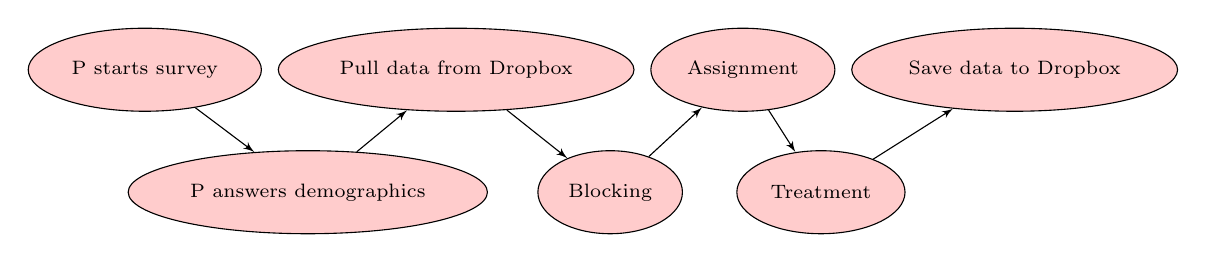
\begin{tikzpicture}
    \node [cloud]  (survey) {\scriptsize{P starts survey}};
    \node [cloud, below right=0.8cm and -0.6cm of survey] (dems) {\scriptsize{P answers demographics}};
    \node [cloud, right= 0.2cm of survey] (pulls) {\scriptsize{Pull data from Dropbox}};
    \node [cloud, below right=0.8cm and -0.3cm of pulls] (blocking) {\scriptsize{Blocking}};
    \node [cloud, right= 0.2cm of pulls] (assignment) {\scriptsize{Assignment}};
    \node [cloud, below right=0.8cm and -0.6cm of assignment] (treatment) {\scriptsize{Treatment}};
    \node [cloud, right= 0.2cm of assignment] (results) {\scriptsize{Save data to Dropbox}};
    \path [line] (survey) -- (dems);
    \path [line] (dems) -- (pulls);
    \path [line] (pulls) -- (blocking);
    \path [line] (blocking) -- (assignment);
    \path [line] (assignment) -- (treatment);
    \path [line] (treatment) -- (results);
\end{tikzpicture}
\caption{Online survey experiment workflow} \label{online-workflow}
\end{figure}
A participant clicks on the survey link and answers the demographic question. After she selects her level of education, \texttt{R} code in the background pulls previous participants' covariate information from a Dropbox server. Based on this information and her chosen education level, the \texttt{R} code sequentially blocks and assigns her to a treatment group. The participant then sees and answers the respective treatment question(s). Her responses are then saved on the same Dropbox server. This process is repeated for all incoming participants. If the participant is the first person to take the survey, i.e.~if there is no covariate information from previous participants yet, the code randomly assigns her to one of the treatment groups. All subsequent participants are then blocked and assigned as just described.

To recruit participants, the cloud-based website can easily be linked to online market platforms, such as MTurk. MTurk is a service where researchers can host tasks to be completed by anonymous participants. Participants receive financial compensation for their work and Amazon collects a commission. MTurk samples have been shown to be internally valid in survey experiments (Berinsky, Huber, \& Lenz, 2012). The use of MTurk in political science experiments has increased dramatically over the past decade and is now common practice (Hauser \& Schwarz, 2016). I use Lucid for my experiment, which has been shown to be equally reliable and performs well on a national scale in survey experiments (Coppock \& McClellan, 2019).

\hypertarget{app-ordmiss}{%
\chapter{ORDINAL MISSING}\label{app-ordmiss}}

\hypertarget{app-ordmiss-allObs}{%
\section{All Observations}\label{app-ordmiss-allObs}}

ANES all obs. 1000 iterations, CCES all obs. 10 iterations (maxed out RAM)
5 variables: Dem, Male, Interest, Inc, Age
MAR (Table \ref{mar.5var.all}) and MNAR (\ref{mnar.5var.all})
\begin{table}[!htbp] \centering 
  \caption{Accuracy of Multiple Imputation Methods. MAR, 5 Variables with NA, all observations} 
  \label{mar.5var.all} 
\begin{threeparttable}
\begin{tabular}{@{\extracolsep{5pt}} D{.}{.}{-3} D{.}{.}{-3} D{.}{.}{-3} D{.}{.}{-3} } 
\\[-1.8ex]\hline 
\hline \\[-1.8ex] 
\multicolumn{1}{c}{Method} & \multicolumn{1}{c}{Variable} & \multicolumn{1}{c}{ANES} & \multicolumn{1}{c}{CCES} \\ 
\hline \\[-1.8ex] 
\multicolumn{1}{c}{true} & \multicolumn{1}{c}{Dem} & \multicolumn{1}{c}{.3370} & \multicolumn{1}{c}{.4032} \\ 
\multicolumn{1}{c}{hot.deck} & \multicolumn{1}{c}{Dem} & \multicolumn{1}{c}{--.0001} & \multicolumn{1}{c}{+.0006} \\ 
\multicolumn{1}{c}{hd.ord} & \multicolumn{1}{c}{Dem} & \multicolumn{1}{c}{--.0002} & \multicolumn{1}{c}{+.0006} \\ 
\multicolumn{1}{c}{amelia} & \multicolumn{1}{c}{Dem} & \multicolumn{1}{c}{+.0000} & \multicolumn{1}{c}{+.0003} \\ 
\multicolumn{1}{c}{mice} & \multicolumn{1}{c}{Dem} & \multicolumn{1}{c}{+.0000} & \multicolumn{1}{c}{+.0003} \\ 
\multicolumn{1}{c}{na.omit} & \multicolumn{1}{c}{Dem} & \multicolumn{1}{c}{--.0302} & \multicolumn{1}{c}{--.0250} \\ 
\multicolumn{1}{c}{true} & \multicolumn{1}{c}{Male} & \multicolumn{1}{c}{.4868} & \multicolumn{1}{c}{.4521} \\ 
\multicolumn{1}{c}{hot.deck} & \multicolumn{1}{c}{Male} & \multicolumn{1}{c}{--.0004} & \multicolumn{1}{c}{--.0001} \\ 
\multicolumn{1}{c}{hd.ord} & \multicolumn{1}{c}{Male} & \multicolumn{1}{c}{--.0008} & \multicolumn{1}{c}{--.0002} \\ 
\multicolumn{1}{c}{amelia} & \multicolumn{1}{c}{Male} & \multicolumn{1}{c}{+.0001} & \multicolumn{1}{c}{+.0001} \\ 
\multicolumn{1}{c}{mice} & \multicolumn{1}{c}{Male} & \multicolumn{1}{c}{+.0001} & \multicolumn{1}{c}{+.0001} \\ 
\multicolumn{1}{c}{na.omit} & \multicolumn{1}{c}{Male} & \multicolumn{1}{c}{--.0365} & \multicolumn{1}{c}{--.0436} \\ 
\multicolumn{1}{c}{true} & \multicolumn{1}{c}{Interest} & \multicolumn{1}{c}{2.8806} & \multicolumn{1}{c}{3.3301} \\ 
\multicolumn{1}{c}{hot.deck} & \multicolumn{1}{c}{Interest} & \multicolumn{1}{c}{--.0087} & \multicolumn{1}{c}{--.0033} \\ 
\multicolumn{1}{c}{hd.ord} & \multicolumn{1}{c}{Interest} & \multicolumn{1}{c}{--.0135} & \multicolumn{1}{c}{--.0046} \\ 
\multicolumn{1}{c}{amelia} & \multicolumn{1}{c}{Interest} & \multicolumn{1}{c}{+.0001} & \multicolumn{1}{c}{+.0001} \\ 
\multicolumn{1}{c}{mice} & \multicolumn{1}{c}{Interest} & \multicolumn{1}{c}{+.0000} & \multicolumn{1}{c}{+.0000} \\ 
\multicolumn{1}{c}{na.omit} & \multicolumn{1}{c}{Interest} & \multicolumn{1}{c}{--.0741} & \multicolumn{1}{c}{--.0763} \\ 
\multicolumn{1}{c}{true} & \multicolumn{1}{c}{Inc} & \multicolumn{1}{c}{16.6894} & \multicolumn{1}{c}{6.5830} \\ 
\multicolumn{1}{c}{hot.deck} & \multicolumn{1}{c}{Inc} & \multicolumn{1}{c}{--.0606} & \multicolumn{1}{c}{--.0009} \\ 
\multicolumn{1}{c}{hd.ord} & \multicolumn{1}{c}{Inc} & \multicolumn{1}{c}{--.1030} & \multicolumn{1}{c}{--.0073} \\ 
\multicolumn{1}{c}{amelia} & \multicolumn{1}{c}{Inc} & \multicolumn{1}{c}{+.0009} & \multicolumn{1}{c}{--.0021} \\ 
\multicolumn{1}{c}{mice} & \multicolumn{1}{c}{Inc} & \multicolumn{1}{c}{--.0007} & \multicolumn{1}{c}{--.0022} \\ 
\multicolumn{1}{c}{na.omit} & \multicolumn{1}{c}{Inc} & \multicolumn{1}{c}{--.5574} & \multicolumn{1}{c}{--.2592} \\ 
\multicolumn{1}{c}{true} & \multicolumn{1}{c}{Age} & \multicolumn{1}{c}{50.3745} & \multicolumn{1}{c}{52.8639} \\ 
\multicolumn{1}{c}{hot.deck} & \multicolumn{1}{c}{Age} & \multicolumn{1}{c}{--.2355} & \multicolumn{1}{c}{--.0221} \\ 
\multicolumn{1}{c}{hd.ord} & \multicolumn{1}{c}{Age} & \multicolumn{1}{c}{--.3698} & \multicolumn{1}{c}{--.0790} \\ 
\multicolumn{1}{c}{amelia} & \multicolumn{1}{c}{Age} & \multicolumn{1}{c}{+.0056} & \multicolumn{1}{c}{--.0006} \\ 
\multicolumn{1}{c}{mice} & \multicolumn{1}{c}{Age} & \multicolumn{1}{c}{+.0053} & \multicolumn{1}{c}{--.0132} \\ 
\multicolumn{1}{c}{na.omit} & \multicolumn{1}{c}{Age} & \multicolumn{1}{c}{--1.2785} & \multicolumn{1}{c}{--1.2190} \\ 
\hline \\[-1.8ex] 
\multicolumn{2}{c}{Observations} & \multicolumn{1}{c}{2395} & \multicolumn{1}{c}{42205} \\ 
\multicolumn{2}{c}{Iterations} & \multicolumn{1}{c}{1000} & \multicolumn{1}{c}{10} \\ 
\hline \\[-1.8ex] 
\end{tabular} 
\begin{tablenotes}[para,flushleft]
\footnotesize{\textit{Note:} Due to the very high number of observations, the CCES data can only be run for a low number of iterations. Anything above that maxes out the 120 GB of RAM available to me. The framing data are not included since their total number of observations (1,003) is virtually identical to the sample of 1,000.}
\end{tablenotes}
\end{threeparttable}
\end{table}
\begin{table}[!htbp] \centering 
  \caption{Accuracy of Multiple Imputation Methods. MNAR, 5 Variables with NA, all observations} 
  \label{mnar.5var.all} 
\begin{threeparttable}
\begin{tabular}{@{\extracolsep{5pt}} D{.}{.}{-3} D{.}{.}{-3} D{.}{.}{-3} D{.}{.}{-3} } 
\\[-1.8ex]\hline 
\hline \\[-1.8ex] 
\multicolumn{1}{c}{Method} & \multicolumn{1}{c}{Variable} & \multicolumn{1}{c}{ANES} & \multicolumn{1}{c}{CCES} \\ 
\hline \\[-1.8ex] 
\multicolumn{1}{c}{true} & \multicolumn{1}{c}{Dem} & \multicolumn{1}{c}{.3370} & \multicolumn{1}{c}{.4032} \\ 
\multicolumn{1}{c}{hot.deck} & \multicolumn{1}{c}{Dem} & \multicolumn{1}{c}{--.0109} & \multicolumn{1}{c}{--.0105} \\ 
\multicolumn{1}{c}{hd.ord} & \multicolumn{1}{c}{Dem} & \multicolumn{1}{c}{--.0113} & \multicolumn{1}{c}{--.0105} \\ 
\multicolumn{1}{c}{amelia} & \multicolumn{1}{c}{Dem} & \multicolumn{1}{c}{--.0110} & \multicolumn{1}{c}{--.0109} \\ 
\multicolumn{1}{c}{mice} & \multicolumn{1}{c}{Dem} & \multicolumn{1}{c}{--.0103} & \multicolumn{1}{c}{--.0106} \\ 
\multicolumn{1}{c}{na.omit} & \multicolumn{1}{c}{Dem} & \multicolumn{1}{c}{--.0185} & \multicolumn{1}{c}{--.0145} \\ 
\multicolumn{1}{c}{true} & \multicolumn{1}{c}{Male} & \multicolumn{1}{c}{.4868} & \multicolumn{1}{c}{.4521} \\ 
\multicolumn{1}{c}{hot.deck} & \multicolumn{1}{c}{Male} & \multicolumn{1}{c}{--.0138} & \multicolumn{1}{c}{--.0129} \\ 
\multicolumn{1}{c}{hd.ord} & \multicolumn{1}{c}{Male} & \multicolumn{1}{c}{--.0136} & \multicolumn{1}{c}{--.0131} \\ 
\multicolumn{1}{c}{amelia} & \multicolumn{1}{c}{Male} & \multicolumn{1}{c}{--.0134} & \multicolumn{1}{c}{--.0132} \\ 
\multicolumn{1}{c}{mice} & \multicolumn{1}{c}{Male} & \multicolumn{1}{c}{--.0134} & \multicolumn{1}{c}{--.0131} \\ 
\multicolumn{1}{c}{na.omit} & \multicolumn{1}{c}{Male} & \multicolumn{1}{c}{--.0196} & \multicolumn{1}{c}{--.0244} \\ 
\multicolumn{1}{c}{true} & \multicolumn{1}{c}{Interest} & \multicolumn{1}{c}{2.8806} & \multicolumn{1}{c}{3.3301} \\ 
\multicolumn{1}{c}{hot.deck} & \multicolumn{1}{c}{Interest} & \multicolumn{1}{c}{--.0257} & \multicolumn{1}{c}{--.0171} \\ 
\multicolumn{1}{c}{hd.ord} & \multicolumn{1}{c}{Interest} & \multicolumn{1}{c}{--.0299} & \multicolumn{1}{c}{--.0179} \\ 
\multicolumn{1}{c}{amelia} & \multicolumn{1}{c}{Interest} & \multicolumn{1}{c}{--.0178} & \multicolumn{1}{c}{--.0147} \\ 
\multicolumn{1}{c}{mice} & \multicolumn{1}{c}{Interest} & \multicolumn{1}{c}{--.0179} & \multicolumn{1}{c}{--.0148} \\ 
\multicolumn{1}{c}{na.omit} & \multicolumn{1}{c}{Interest} & \multicolumn{1}{c}{--.0407} & \multicolumn{1}{c}{--.0418} \\ 
\multicolumn{1}{c}{true} & \multicolumn{1}{c}{Inc} & \multicolumn{1}{c}{16.6894} & \multicolumn{1}{c}{6.5830} \\ 
\multicolumn{1}{c}{hot.deck} & \multicolumn{1}{c}{Inc} & \multicolumn{1}{c}{--.1874} & \multicolumn{1}{c}{--.0691} \\ 
\multicolumn{1}{c}{hd.ord} & \multicolumn{1}{c}{Inc} & \multicolumn{1}{c}{--.2287} & \multicolumn{1}{c}{--.0696} \\ 
\multicolumn{1}{c}{amelia} & \multicolumn{1}{c}{Inc} & \multicolumn{1}{c}{--.1292} & \multicolumn{1}{c}{--.0637} \\ 
\multicolumn{1}{c}{mice} & \multicolumn{1}{c}{Inc} & \multicolumn{1}{c}{--.1297} & \multicolumn{1}{c}{--.0634} \\ 
\multicolumn{1}{c}{na.omit} & \multicolumn{1}{c}{Inc} & \multicolumn{1}{c}{--.2729} & \multicolumn{1}{c}{--.1375} \\ 
\multicolumn{1}{c}{true} & \multicolumn{1}{c}{Age} & \multicolumn{1}{c}{50.3745} & \multicolumn{1}{c}{52.8639} \\ 
\multicolumn{1}{c}{hot.deck} & \multicolumn{1}{c}{Age} & \multicolumn{1}{c}{--.5240} & \multicolumn{1}{c}{--.2331} \\ 
\multicolumn{1}{c}{hd.ord} & \multicolumn{1}{c}{Age} & \multicolumn{1}{c}{--.6609} & \multicolumn{1}{c}{--.2764} \\ 
\multicolumn{1}{c}{amelia} & \multicolumn{1}{c}{Age} & \multicolumn{1}{c}{--.2533} & \multicolumn{1}{c}{--.2342} \\ 
\multicolumn{1}{c}{mice} & \multicolumn{1}{c}{Age} & \multicolumn{1}{c}{--.2474} & \multicolumn{1}{c}{--.2371} \\ 
\multicolumn{1}{c}{na.omit} & \multicolumn{1}{c}{Age} & \multicolumn{1}{c}{--.7188} & \multicolumn{1}{c}{--.6476} \\ 
\hline \\[-1.8ex] 
\multicolumn{2}{c}{Observations} & \multicolumn{1}{c}{2395} & \multicolumn{1}{c}{42205} \\ 
\multicolumn{2}{c}{Iterations} & \multicolumn{1}{c}{1000} & \multicolumn{1}{c}{10} \\ 
\hline \\[-1.8ex] 
\end{tabular} 
\begin{tablenotes}[para,flushleft]
\footnotesize{\textit{Note:} Due to the very high number of observations, the CCES data can only be run for a low number of iterations. Anything above that maxes out the 120 GB of RAM available to me. The framing data are not included since their total number of observations (1,003) is virtually identical to the sample of 1,000.}
\end{tablenotes}
\end{threeparttable}
\end{table}
\clearpage

\hypertarget{app-ordmiss-increaseNA}{%
\section{Increased Missingness}\label{app-ordmiss-increaseNA}}

CCES 10,000 iterations +++
5 variables: Dem, Male, Interest, Inc, Age
MAR
20, 50, 80 percent

\hypertarget{app-ordmiss-speed}{%
\section{Speed}\label{app-ordmiss-speed}}

CCES 10,000 iterations +++
5 variables: Dem, Male, Interest, Inc, Age
MAR
20, 50, 80 percent
\begin{table}[!htbp] \centering 
  \caption{Runtimes of Multiple Imputation Methods (in Minutes) with All Available Observations} 
  \label{run.all.obs} 
\begin{threeparttable}
\begin{tabular}{@{\extracolsep{5pt}} D{.}{.}{-3} D{.}{.}{-3} D{.}{.}{-3} } 
\\[-1.8ex]\hline 
\hline \\[-1.8ex] 
\multicolumn{1}{c}{Method} & \multicolumn{1}{c}{ANES} & \multicolumn{1}{c}{CCES} \\ 
\hline \\[-1.8ex] 
\multicolumn{1}{c}{hd.ord} & \multicolumn{1}{c}{9.406} & \multicolumn{1}{c}{21.829} \\ 
\multicolumn{1}{c}{hot.deck} & \multicolumn{1}{c}{9.374} & \multicolumn{1}{c}{21.429} \\ 
\multicolumn{1}{c}{amelia} & \multicolumn{1}{c}{12.393} & \multicolumn{1}{c}{2.602} \\ 
\multicolumn{1}{c}{mice} & \multicolumn{1}{c}{99.455} & \multicolumn{1}{c}{100.253} \\ 
\hline \\[-1.8ex] 
\multicolumn{1}{c}{Observations} & \multicolumn{1}{c}{2395} & \multicolumn{1}{c}{42205} \\ 
\multicolumn{1}{c}{Iterations} & \multicolumn{1}{c}{1000} & \multicolumn{1}{c}{10} \\ 
\hline \\[-1.8ex] 
\end{tabular} 
\begin{tablenotes}[para,flushleft]
\footnotesize{\textit{Note:} Due to the very high number of observations, the CCES data can only be run for a low number of iterations. Anything above that maxes out the 120 GB of RAM available to me. The framing data are not included since their total number of observations (1,003) is virtually identical to the sample of 1,000.}
\end{tablenotes}
\end{threeparttable}
\end{table}
\hypertarget{app-ordmiss-modified.ampute}{%
\section{\texorpdfstring{With Modified \texttt{ampute()}}{With Modified ampute()}}\label{app-ordmiss-modified.ampute}}

Table \ref{amp.oldframe.bycases.acc} shows the results of using \texttt{ampute()} with the options \texttt{bycases=FALSE} and \texttt{cont=FALSE} on the old framing data (n = 1,003) and inserts NAs MAR for 5 variables at 20 percent for 9,644 iterations. \texttt{hd.ord} overall performs worse in this scenario.
\begin{table}[!htbp] \centering 
  \caption{Accuracy of Multiple Imputation Method. ampute() with bycases, old framing data (n = 1,003)} 
  \label{amp.oldframe.bycases.acc} 
\begin{tabular}{@{\extracolsep{5pt}} D{.}{.}{-4} D{.}{.}{-4} D{.}{.}{-4} D{.}{.}{-4} } 
\\[-1.8ex]\hline 
\hline \\[-1.8ex] 
\multicolumn{1}{c}{Method} & \multicolumn{1}{c}{Variable} & \multicolumn{1}{c}{Value} & \multicolumn{1}{c}{Diff} \\ 
\hline \\[-1.8ex] 
\multicolumn{1}{c}{true} & \multicolumn{1}{c}{Dem} & \multicolumn{1}{c}{.4666} & \multicolumn{1}{c}{.0000} \\ 
\multicolumn{1}{c}{hd.ord} & \multicolumn{1}{c}{Dem} & \multicolumn{1}{c}{.4674} & \multicolumn{1}{c}{.0008} \\ 
\multicolumn{1}{c}{hd.norm} & \multicolumn{1}{c}{Dem} & \multicolumn{1}{c}{.4686} & \multicolumn{1}{c}{.0020} \\ 
\multicolumn{1}{c}{amelia} & \multicolumn{1}{c}{Dem} & \multicolumn{1}{c}{.4669} & \multicolumn{1}{c}{.0003} \\ 
\multicolumn{1}{c}{mice} & \multicolumn{1}{c}{Dem} & \multicolumn{1}{c}{.4667} & \multicolumn{1}{c}{.0001} \\ 
\multicolumn{1}{c}{na.omit} & \multicolumn{1}{c}{Dem} & \multicolumn{1}{c}{.2363} & \multicolumn{1}{c}{.2303} \\ 
\multicolumn{1}{c}{true} & \multicolumn{1}{c}{inc} & \multicolumn{1}{c}{3.0927} & \multicolumn{1}{c}{.0000} \\ 
\multicolumn{1}{c}{hd.ord} & \multicolumn{1}{c}{inc} & \multicolumn{1}{c}{3.0466} & \multicolumn{1}{c}{.0461} \\ 
\multicolumn{1}{c}{hd.norm} & \multicolumn{1}{c}{inc} & \multicolumn{1}{c}{3.0245} & \multicolumn{1}{c}{.0682} \\ 
\multicolumn{1}{c}{amelia} & \multicolumn{1}{c}{inc} & \multicolumn{1}{c}{3.0941} & \multicolumn{1}{c}{.0014} \\ 
\multicolumn{1}{c}{mice} & \multicolumn{1}{c}{inc} & \multicolumn{1}{c}{3.0973} & \multicolumn{1}{c}{.0046} \\ 
\multicolumn{1}{c}{na.omit} & \multicolumn{1}{c}{inc} & \multicolumn{1}{c}{2.4208} & \multicolumn{1}{c}{.6719} \\ 
\multicolumn{1}{c}{true} & \multicolumn{1}{c}{age} & \multicolumn{1}{c}{37.9252} & \multicolumn{1}{c}{.0000} \\ 
\multicolumn{1}{c}{hd.ord} & \multicolumn{1}{c}{age} & \multicolumn{1}{c}{36.5063} & \multicolumn{1}{c}{1.4189} \\ 
\multicolumn{1}{c}{hd.norm} & \multicolumn{1}{c}{age} & \multicolumn{1}{c}{36.3438} & \multicolumn{1}{c}{1.5814} \\ 
\multicolumn{1}{c}{amelia} & \multicolumn{1}{c}{age} & \multicolumn{1}{c}{37.9287} & \multicolumn{1}{c}{.0035} \\ 
\multicolumn{1}{c}{mice} & \multicolumn{1}{c}{age} & \multicolumn{1}{c}{37.9398} & \multicolumn{1}{c}{.0146} \\ 
\multicolumn{1}{c}{na.omit} & \multicolumn{1}{c}{age} & \multicolumn{1}{c}{31.6958} & \multicolumn{1}{c}{6.2294} \\ 
\multicolumn{1}{c}{true} & \multicolumn{1}{c}{Female} & \multicolumn{1}{c}{.4666} & \multicolumn{1}{c}{.0000} \\ 
\multicolumn{1}{c}{hd.ord} & \multicolumn{1}{c}{Female} & \multicolumn{1}{c}{.4619} & \multicolumn{1}{c}{.0047} \\ 
\multicolumn{1}{c}{hd.norm} & \multicolumn{1}{c}{Female} & \multicolumn{1}{c}{.4600} & \multicolumn{1}{c}{.0066} \\ 
\multicolumn{1}{c}{amelia} & \multicolumn{1}{c}{Female} & \multicolumn{1}{c}{.4663} & \multicolumn{1}{c}{.0003} \\ 
\multicolumn{1}{c}{mice} & \multicolumn{1}{c}{Female} & \multicolumn{1}{c}{.4666} & \multicolumn{1}{c}{.0000} \\ 
\multicolumn{1}{c}{na.omit} & \multicolumn{1}{c}{Female} & \multicolumn{1}{c}{.2168} & \multicolumn{1}{c}{.2498} \\ 
\multicolumn{1}{c}{true} & \multicolumn{1}{c}{interest} & \multicolumn{1}{c}{3.2164} & \multicolumn{1}{c}{.0000} \\ 
\multicolumn{1}{c}{hd.ord} & \multicolumn{1}{c}{interest} & \multicolumn{1}{c}{3.1362} & \multicolumn{1}{c}{.0802} \\ 
\multicolumn{1}{c}{hd.norm} & \multicolumn{1}{c}{interest} & \multicolumn{1}{c}{3.1223} & \multicolumn{1}{c}{.0941} \\ 
\multicolumn{1}{c}{amelia} & \multicolumn{1}{c}{interest} & \multicolumn{1}{c}{3.2150} & \multicolumn{1}{c}{.0014} \\ 
\multicolumn{1}{c}{mice} & \multicolumn{1}{c}{interest} & \multicolumn{1}{c}{3.2147} & \multicolumn{1}{c}{.0017} \\ 
\multicolumn{1}{c}{na.omit} & \multicolumn{1}{c}{interest} & \multicolumn{1}{c}{2.7280} & \multicolumn{1}{c}{.4884} \\ 
\hline \\[-1.8ex] 
\end{tabular} 
\end{table}
\hypertarget{app-ordmiss-own}{%
\section{With My Own Amputation Methods}\label{app-ordmiss-own}}

Table \ref{own.NA.oldframe.acc} shows the results of using my own function, \texttt{own.NA()}, to insert 20 percent NAs MAR into three variables in the old framing data (n = 1,003). In general, something is MAR if you ampute values in column A based on values in column B, e.g.~if you ampute the values for \texttt{age} where \texttt{income\ =\ 1} and where \texttt{income\ =\ 5}. \texttt{own.NA()} applies this procedure for any combination of columns. Here, the chosen columns to be amputed are \texttt{Dem}, \texttt{age}, and \texttt{interest}. The chosen columns the amputations depend on are \texttt{inc}, \texttt{Female}, and \texttt{Black}. The function samples 20 percent of observations for each unique value of \texttt{inc}. For those observations, the values of \texttt{Dem} are amputed. Accordingly, the function samples 20 percent of observations for each unique value of \texttt{Female}. For those observations, the values of \texttt{age} are amputed. The same occurs for \texttt{Black} and \texttt{interest}. The resulting data frame is then imputed. Note that the number of amputed and imputed variables is generally lower, as a pair of variables is needed to ampute one variable. As Table \ref{own.NA.oldframe.acc} shows, \texttt{hd.ord} does not perform particularly well. It beats \texttt{hd.norm} for all three variables but falls considerably short of \texttt{amelia} and \texttt{mice}. It is notable, however, that my method seems closer to being MCAR than MAR, as \texttt{na.omit} performs well and sometimes even outperforms other methods, for instance for \texttt{interest}. It is thus questionable how much use \texttt{own.NA()} is in its current form.
\begin{table}[!htbp] \centering 
  \caption{Accuracy of Multiple Imputation Methods. own.NA(), old framing data (n = 1,003)} 
  \label{own.NA.oldframe.acc} 
\begin{tabular}{@{\extracolsep{5pt}} D{.}{.}{-4} D{.}{.}{-4} D{.}{.}{-4} D{.}{.}{-4} } 
\\[-1.8ex]\hline 
\hline \\[-1.8ex] 
\multicolumn{1}{c}{Method} & \multicolumn{1}{c}{Variable} & \multicolumn{1}{c}{Value} & \multicolumn{1}{c}{Diff} \\ 
\hline \\[-1.8ex] 
\multicolumn{1}{c}{true} & \multicolumn{1}{c}{Dem} & \multicolumn{1}{c}{.4666} & \multicolumn{1}{c}{.0000} \\ 
\multicolumn{1}{c}{hd.ord} & \multicolumn{1}{c}{Dem} & \multicolumn{1}{c}{.4695} & \multicolumn{1}{c}{.0029} \\ 
\multicolumn{1}{c}{hd.norm} & \multicolumn{1}{c}{Dem} & \multicolumn{1}{c}{.4721} & \multicolumn{1}{c}{.0055} \\ 
\multicolumn{1}{c}{amelia} & \multicolumn{1}{c}{Dem} & \multicolumn{1}{c}{.4667} & \multicolumn{1}{c}{.0001} \\ 
\multicolumn{1}{c}{mice} & \multicolumn{1}{c}{Dem} & \multicolumn{1}{c}{.4669} & \multicolumn{1}{c}{.0003} \\ 
\multicolumn{1}{c}{na.omit} & \multicolumn{1}{c}{Dem} & \multicolumn{1}{c}{.4668} & \multicolumn{1}{c}{.0002} \\ 
\multicolumn{1}{c}{true} & \multicolumn{1}{c}{age} & \multicolumn{1}{c}{37.9252} & \multicolumn{1}{c}{.0000} \\ 
\multicolumn{1}{c}{hd.ord} & \multicolumn{1}{c}{age} & \multicolumn{1}{c}{36.1537} & \multicolumn{1}{c}{1.7715} \\ 
\multicolumn{1}{c}{hd.norm} & \multicolumn{1}{c}{age} & \multicolumn{1}{c}{35.8843} & \multicolumn{1}{c}{2.0409} \\ 
\multicolumn{1}{c}{amelia} & \multicolumn{1}{c}{age} & \multicolumn{1}{c}{37.9245} & \multicolumn{1}{c}{.0007} \\ 
\multicolumn{1}{c}{mice} & \multicolumn{1}{c}{age} & \multicolumn{1}{c}{37.9371} & \multicolumn{1}{c}{.0119} \\ 
\multicolumn{1}{c}{na.omit} & \multicolumn{1}{c}{age} & \multicolumn{1}{c}{37.9221} & \multicolumn{1}{c}{.0031} \\ 
\multicolumn{1}{c}{true} & \multicolumn{1}{c}{interest} & \multicolumn{1}{c}{3.2164} & \multicolumn{1}{c}{.0000} \\ 
\multicolumn{1}{c}{hd.ord} & \multicolumn{1}{c}{interest} & \multicolumn{1}{c}{3.1160} & \multicolumn{1}{c}{.1004} \\ 
\multicolumn{1}{c}{hd.norm} & \multicolumn{1}{c}{interest} & \multicolumn{1}{c}{3.1012} & \multicolumn{1}{c}{.1152} \\ 
\multicolumn{1}{c}{amelia} & \multicolumn{1}{c}{interest} & \multicolumn{1}{c}{3.2166} & \multicolumn{1}{c}{.0002} \\ 
\multicolumn{1}{c}{mice} & \multicolumn{1}{c}{interest} & \multicolumn{1}{c}{3.2156} & \multicolumn{1}{c}{.0008} \\ 
\multicolumn{1}{c}{na.omit} & \multicolumn{1}{c}{interest} & \multicolumn{1}{c}{3.2165} & \multicolumn{1}{c}{.0001} \\ 
\hline \\[-1.8ex] 
\end{tabular} 
\end{table}
\texttt{ampute()} seems to spread NAs evenly across columns. This means that observations are mostly complete, with not more than one or two missing values. I wrote another function, \texttt{own.NA.rows()}, that changes this. \texttt{own.NA.rows()} inserts missingness for a percentage of observations MAR across all columns except \texttt{education}. This means that the majority of observations are complete but a percentage of observations misses data on almost all variables. Table \ref{own.NA.rows.oldframe.acc} shows the results, with the missingess percentage set to 20 and NAs inserted into 17 variables.

\ssp
\begin{longtable}{@{\extracolsep{5pt}} D{.}{.}{-4} D{.}{.}{-4} D{.}{.}{-4} D{.}{.}{-4} } 
  \caption{Accuracy of Multiple Imputation Methods. own.NA.rows(), old framing data (n = 1,003)} 
  \label{own.NA.rows.oldframe.acc} 
\\[-1.8ex]\hline 
\hline \\[-1.8ex] 
\multicolumn{1}{c}{Method} & \multicolumn{1}{c}{Variable} & \multicolumn{1}{c}{Value} & \multicolumn{1}{c}{Diff} \\ 
\hline \\[-1.8ex] 
\multicolumn{1}{c}{true} & \multicolumn{1}{c}{Dem} & .4666 & 0 \\ 
\multicolumn{1}{c}{hd.ord} & \multicolumn{1}{c}{Dem} & .4666 & 0 \\ 
\multicolumn{1}{c}{hd.norm} & \multicolumn{1}{c}{Dem} & .4667 & .0001 \\ 
\multicolumn{1}{c}{amelia} & \multicolumn{1}{c}{Dem} & .4667 & .0001 \\ 
\multicolumn{1}{c}{mice} & \multicolumn{1}{c}{Dem} & .4670 & .0004 \\ 
\multicolumn{1}{c}{na.omit} & \multicolumn{1}{c}{Dem} & .4667 & .0001 \\ 
\multicolumn{1}{c}{true} & \multicolumn{1}{c}{Ind} & .2802 & 0 \\ 
\multicolumn{1}{c}{hd.ord} & \multicolumn{1}{c}{Ind} & .2795 & .0007 \\ 
\multicolumn{1}{c}{hd.norm} & \multicolumn{1}{c}{Ind} & .2801 & .0001 \\ 
\multicolumn{1}{c}{amelia} & \multicolumn{1}{c}{Ind} & .2801 & .0001 \\ 
\multicolumn{1}{c}{mice} & \multicolumn{1}{c}{Ind} & .2817 & .0015 \\ 
\multicolumn{1}{c}{na.omit} & \multicolumn{1}{c}{Ind} & .2801 & .0001 \\ 
\multicolumn{1}{c}{true} & \multicolumn{1}{c}{Cons} & .2832 & 0 \\ 
\multicolumn{1}{c}{hd.ord} & \multicolumn{1}{c}{Cons} & .2830 & .0002 \\ 
\multicolumn{1}{c}{hd.norm} & \multicolumn{1}{c}{Cons} & .2831 & .0001 \\ 
\multicolumn{1}{c}{amelia} & \multicolumn{1}{c}{Cons} & .2831 & .0001 \\ 
\multicolumn{1}{c}{mice} & \multicolumn{1}{c}{Cons} & .2823 & .0009 \\ 
\multicolumn{1}{c}{na.omit} & \multicolumn{1}{c}{Cons} & .2831 & .0001 \\ 
\multicolumn{1}{c}{true} & \multicolumn{1}{c}{Lib} & .5174 & 0 \\ 
\multicolumn{1}{c}{hd.ord} & \multicolumn{1}{c}{Lib} & .5182 & .0008 \\ 
\multicolumn{1}{c}{hd.norm} & \multicolumn{1}{c}{Lib} & .5176 & .0002 \\ 
\multicolumn{1}{c}{amelia} & \multicolumn{1}{c}{Lib} & .5176 & .0002 \\ 
\multicolumn{1}{c}{mice} & \multicolumn{1}{c}{Lib} & .5173 & .0001 \\ 
\multicolumn{1}{c}{na.omit} & \multicolumn{1}{c}{Lib} & .5176 & .0002 \\ 
\multicolumn{1}{c}{true} & \multicolumn{1}{c}{Black} & .0698 & 0 \\ 
\multicolumn{1}{c}{hd.ord} & \multicolumn{1}{c}{Black} & .0702 & .0004 \\ 
\multicolumn{1}{c}{hd.norm} & \multicolumn{1}{c}{Black} & .0698 & 0 \\ 
\multicolumn{1}{c}{amelia} & \multicolumn{1}{c}{Black} & .0698 & 0 \\ 
\multicolumn{1}{c}{mice} & \multicolumn{1}{c}{Black} & .0731 & .0033 \\ 
\multicolumn{1}{c}{na.omit} & \multicolumn{1}{c}{Black} & .0698 & 0 \\ 
\multicolumn{1}{c}{true} & \multicolumn{1}{c}{Hisp} & .0548 & 0 \\ 
\multicolumn{1}{c}{hd.ord} & \multicolumn{1}{c}{Hisp} & .0546 & .0002 \\ 
\multicolumn{1}{c}{hd.norm} & \multicolumn{1}{c}{Hisp} & .0548 & 0 \\ 
\multicolumn{1}{c}{amelia} & \multicolumn{1}{c}{Hisp} & .0548 & 0 \\ 
\multicolumn{1}{c}{mice} & \multicolumn{1}{c}{Hisp} & .0589 & .0041 \\ 
\multicolumn{1}{c}{na.omit} & \multicolumn{1}{c}{Hisp} & .0548 & 0 \\ 
\multicolumn{1}{c}{true} & \multicolumn{1}{c}{White} & .7717 & 0 \\ 
\multicolumn{1}{c}{hd.ord} & \multicolumn{1}{c}{White} & .7712 & .0005 \\ 
\multicolumn{1}{c}{hd.norm} & \multicolumn{1}{c}{White} & .7717 & 0 \\ 
\multicolumn{1}{c}{amelia} & \multicolumn{1}{c}{White} & .7717 & 0 \\ 
\multicolumn{1}{c}{mice} & \multicolumn{1}{c}{White} & .7613 & .0104 \\ 
\multicolumn{1}{c}{na.omit} & \multicolumn{1}{c}{White} & .7717 & 0 \\ 
\multicolumn{1}{c}{true} & \multicolumn{1}{c}{Asian} & .0808 & 0 \\ 
\multicolumn{1}{c}{hd.ord} & \multicolumn{1}{c}{Asian} & .0812 & .0004 \\ 
\multicolumn{1}{c}{hd.norm} & \multicolumn{1}{c}{Asian} & .0808 & 0 \\ 
\multicolumn{1}{c}{amelia} & \multicolumn{1}{c}{Asian} & .0809 & .0001 \\ 
\multicolumn{1}{c}{mice} & \multicolumn{1}{c}{Asian} & .0835 & .0027 \\ 
\multicolumn{1}{c}{na.omit} & \multicolumn{1}{c}{Asian} & .0808 & 0 \\ 
\multicolumn{1}{c}{true} & \multicolumn{1}{c}{Female} & .4666 & 0 \\ 
\multicolumn{1}{c}{hd.ord} & \multicolumn{1}{c}{Female} & .4665 & .0001 \\ 
\multicolumn{1}{c}{hd.norm} & \multicolumn{1}{c}{Female} & .4665 & .0001 \\ 
\multicolumn{1}{c}{amelia} & \multicolumn{1}{c}{Female} & .4665 & .0001 \\ 
\multicolumn{1}{c}{mice} & \multicolumn{1}{c}{Female} & .4673 & .0007 \\ 
\multicolumn{1}{c}{na.omit} & \multicolumn{1}{c}{Female} & .4665 & .0001 \\ 
\multicolumn{1}{c}{true} & \multicolumn{1}{c}{Unempl} & .1615 & 0 \\ 
\multicolumn{1}{c}{hd.ord} & \multicolumn{1}{c}{Unempl} & .1610 & .0005 \\ 
\multicolumn{1}{c}{hd.norm} & \multicolumn{1}{c}{Unempl} & .1616 & .0001 \\ 
\multicolumn{1}{c}{amelia} & \multicolumn{1}{c}{Unempl} & .1616 & .0001 \\ 
\multicolumn{1}{c}{mice} & \multicolumn{1}{c}{Unempl} & .1624 & .0009 \\ 
\multicolumn{1}{c}{na.omit} & \multicolumn{1}{c}{Unempl} & .1616 & .0001 \\ 
\multicolumn{1}{c}{true} & \multicolumn{1}{c}{Ret} & .0508 & 0 \\ 
\multicolumn{1}{c}{hd.ord} & \multicolumn{1}{c}{Ret} & .0506 & .0002 \\ 
\multicolumn{1}{c}{hd.norm} & \multicolumn{1}{c}{Ret} & .0508 & 0 \\ 
\multicolumn{1}{c}{amelia} & \multicolumn{1}{c}{Ret} & .0509 & .0001 \\ 
\multicolumn{1}{c}{mice} & \multicolumn{1}{c}{Ret} & .0505 & .0003 \\ 
\multicolumn{1}{c}{na.omit} & \multicolumn{1}{c}{Ret} & .0509 & .0001 \\ 
\multicolumn{1}{c}{true} & \multicolumn{1}{c}{Stud} & .0439 & 0 \\ 
\multicolumn{1}{c}{hd.ord} & \multicolumn{1}{c}{Stud} & .0446 & .0007 \\ 
\multicolumn{1}{c}{hd.norm} & \multicolumn{1}{c}{Stud} & .0439 & 0 \\ 
\multicolumn{1}{c}{amelia} & \multicolumn{1}{c}{Stud} & .0439 & 0 \\ 
\multicolumn{1}{c}{mice} & \multicolumn{1}{c}{Stud} & .0466 & .0027 \\ 
\multicolumn{1}{c}{na.omit} & \multicolumn{1}{c}{Stud} & .0439 & 0 \\ 
\multicolumn{1}{c}{true} & \multicolumn{1}{c}{interest} & 3.2164 & 0 \\ 
\multicolumn{1}{c}{hd.ord} & \multicolumn{1}{c}{interest} & 3.2161 & .0003 \\ 
\multicolumn{1}{c}{hd.norm} & \multicolumn{1}{c}{interest} & 3.2163 & .0001 \\ 
\multicolumn{1}{c}{amelia} & \multicolumn{1}{c}{interest} & 3.2164 & 0 \\ 
\multicolumn{1}{c}{mice} & \multicolumn{1}{c}{interest} & 3.2122 & .0042 \\ 
\multicolumn{1}{c}{na.omit} & \multicolumn{1}{c}{interest} & 3.2163 & .0001 \\ 
\multicolumn{1}{c}{true} & \multicolumn{1}{c}{media} & 1.7268 & 0 \\ 
\multicolumn{1}{c}{hd.ord} & \multicolumn{1}{c}{media} & 1.7294 & .0026 \\ 
\multicolumn{1}{c}{hd.norm} & \multicolumn{1}{c}{media} & 1.7270 & .0002 \\ 
\multicolumn{1}{c}{amelia} & \multicolumn{1}{c}{media} & 1.7270 & .0002 \\ 
\multicolumn{1}{c}{mice} & \multicolumn{1}{c}{media} & 1.7259 & .0009 \\ 
\multicolumn{1}{c}{na.omit} & \multicolumn{1}{c}{media} & 1.7269 & .0001 \\ 
\multicolumn{1}{c}{true} & \multicolumn{1}{c}{part} & .9561 & 0 \\ 
\multicolumn{1}{c}{hd.ord} & \multicolumn{1}{c}{part} & .9575 & .0014 \\ 
\multicolumn{1}{c}{hd.norm} & \multicolumn{1}{c}{part} & .9560 & .0001 \\ 
\multicolumn{1}{c}{amelia} & \multicolumn{1}{c}{part} & .9561 & 0 \\ 
\multicolumn{1}{c}{mice} & \multicolumn{1}{c}{part} & .9546 & .0015 \\ 
\multicolumn{1}{c}{na.omit} & \multicolumn{1}{c}{part} & .9561 & 0 \\ 
\multicolumn{1}{c}{true} & \multicolumn{1}{c}{inc} & 3.0927 & 0 \\ 
\multicolumn{1}{c}{hd.ord} & \multicolumn{1}{c}{inc} & 3.0906 & .0021 \\ 
\multicolumn{1}{c}{hd.norm} & \multicolumn{1}{c}{inc} & 3.0926 & .0001 \\ 
\multicolumn{1}{c}{amelia} & \multicolumn{1}{c}{inc} & 3.0926 & .0001 \\ 
\multicolumn{1}{c}{mice} & \multicolumn{1}{c}{inc} & 3.0949 & .0022 \\ 
\multicolumn{1}{c}{na.omit} & \multicolumn{1}{c}{inc} & 3.0926 & .0001 \\ 
\multicolumn{1}{c}{true} & \multicolumn{1}{c}{age} & 37.9252 & 0 \\ 
\multicolumn{1}{c}{hd.ord} & \multicolumn{1}{c}{age} & 37.9000 & .0252 \\ 
\multicolumn{1}{c}{hd.norm} & \multicolumn{1}{c}{age} & 37.9250 & .0002 \\ 
\multicolumn{1}{c}{amelia} & \multicolumn{1}{c}{age} & 37.9243 & .0009 \\ 
\multicolumn{1}{c}{mice} & \multicolumn{1}{c}{age} & 37.8789 & .0463 \\ 
\multicolumn{1}{c}{na.omit} & \multicolumn{1}{c}{age} & 37.9250 & .0002 \\ 
\hline \\[-1.8ex] 
\end{longtable}
\dsp

\texttt{hd.norm}, \texttt{amelia}, and \texttt{na.omit} perform very well. No difference to the true value for any variable is greater than .0009 and most are .0002.

\texttt{hd.ord} performs on similar levels except for the nominal variables (\texttt{media} (.0026), \texttt{part} (.0014), \texttt{inc} (.0021), \texttt{age} (.0252)).

Somewhat surprisingly, \texttt{mice} performs worst overall for many variables (\texttt{Ind} (.0015), \texttt{Black} (.0033), \texttt{Hisp} (.0041), \texttt{White} (.0104), \texttt{Asian} (.0027), \texttt{Stud} (.0027), \texttt{interest} (.0042), \texttt{part} (.0015), \texttt{inc} (.0022), \texttt{age} (.0463)) by some margin.

It is also noteable how often the difference amounts to zero and how well \texttt{na.omit} performs overall.

\hypertarget{references}{%
\chapter*{REFERENCES}\label{references}}
\addcontentsline{toc}{chapter}{REFERENCES}

\noindent

\ssp

\hypertarget{refs}{}
\leavevmode\hypertarget{ref-aaroe_investigating_2011}{}%
Aaroe, L. (2011). Investigating Frame Strength: The Case of Episodic and Thematic Frames. \emph{Political Communication}, \emph{28}(2), 207--226.

\leavevmode\hypertarget{ref-abramowitz_disappearing_2010}{}%
Abramowitz, A. I. (2010). \emph{The Disappearing Center: Engaged Citizens, Polarization, and American Democracy}. New Haven, CT: Yale University Press.

\leavevmode\hypertarget{ref-agresti_1990_categorical}{}%
Agresti, A. (1990). \emph{Categorical data analysis}. Hoboken, NJ: Wiley-Interscience.

\leavevmode\hypertarget{ref-agresti_1996_introduction}{}%
Agresti, A. (1996). \emph{An Introduction to Categorical Data Analysis}. Hoboken, NJ: Wiley-Interscience.

\leavevmode\hypertarget{ref-agresti_2010_analysis}{}%
Agresti, A. (2010). \emph{Analysis of ordinal categorical data} (2nd ed.). Hoboken, NJ: Wiley-Interscience.

\leavevmode\hypertarget{ref-allison_2002_missing}{}%
Allison, P. D. (2002). \emph{Missing Data}. Thousand Oaks, CA: SAGE Publications.

\leavevmode\hypertarget{ref-andsager_how_2000}{}%
Andsager, J. (2000). How Interest Groups Attempt to Shape Public Opinion with Competing News Frames. \emph{Journalism and Mass Communication Quarterly}, \emph{77}(3), 577--592.

\leavevmode\hypertarget{ref-arceneaux_cognitive_2012}{}%
Arceneaux, K. (2012). Cognitive Biases and the Strength of Political Arguments. \emph{American Journal of Political Science}, \emph{56}(2), 271--285.

\leavevmode\hypertarget{ref-barari_2017_package}{}%
Barari, S., Berwick, E., Hainmueller, J., Hopkins, D. J., Liu, S., Strezhnev, A., \& Yamamoto, T. (2017). \emph{Package ``cjoint''}. https://cran.r-project.org/web/packages/cjoint/cjoint.pdf, package version 2.0.6.

\leavevmode\hypertarget{ref-baron_protected_1997}{}%
Baron, J., \& Spranca, M. (1997). Protected Values. \emph{Organizational Behavior and Human Decision Processes}, \emph{70}, 1--16.

\leavevmode\hypertarget{ref-bennis_costs_2010}{}%
Bennis, W. M., Medin, D. L., \& Bartels, D. M. (2010). The Costs and Benefits of Calculation and Moral Rules. \emph{Perspectives on Psychological Science}, \emph{5}, 187--202.

\leavevmode\hypertarget{ref-berinsky_evaluating_2012}{}%
Berinsky, A. J., Huber, G. A., \& Lenz, G. S. (2012). Evaluating Online Labor Markets for Experimental Research: Amazon.Com's Mechanical Turk. \emph{Political Analysis}, \emph{20}(3), 351--368.

\leavevmode\hypertarget{ref-boas_fielding_2013}{}%
Boas, T. C., \& Hidalgo, F. D. (2013). Fielding Complex Online Surveys Using rApache and Qualtrics. \emph{The Political Methodologist}, \emph{20}(2), 21--26.

\leavevmode\hypertarget{ref-brewer_values_2005}{}%
Brewer, P., \& Gross, K. (2005). Values, Framing, and Citizens' Thoughts About Policy Issues: Effects on Content and Quantity. \emph{Political Psychology}, \emph{26}(6), 929--948.

\leavevmode\hypertarget{ref-callaghan_introduction_2005}{}%
Callaghan, K., \& Schnell, F. (2005). Introduction: Framing Political Issues in American Politics. In K. Callaghan \& F. Schnell (Eds.), \emph{Framing American politics} (pp. 1--17). Pittsburgh, PA: University of Pittsburgh Press.

\leavevmode\hypertarget{ref-carpini_1993_measuring}{}%
Carpini, M. X. D., \& Keeter, S. (1993). Measuring political knowledge: Putting first things first. \emph{American Journal of Political Science}, \emph{37}(4), 1179--1206.

\leavevmode\hypertarget{ref-chong_framing_2007}{}%
Chong, D., \& Druckman, J. (2007). Framing Public Opinion in Competitive Democracies. \emph{American Political Science Review}, \emph{101}(4), 637--655.

\leavevmode\hypertarget{ref-chong_dynamic_2010}{}%
Chong, D., \& Druckman, J. (2010). Dynamic Public Opinion: Communication Effects Over Time. \emph{American Political Science Review}, \emph{104}(4), 663--680.

\leavevmode\hypertarget{ref-chong_counterframing_2013}{}%
Chong, D., \& Druckman, J. (2013). Counterframing Effects. \emph{Journal of Politics}, \emph{75}(1), 1--16.

\leavevmode\hypertarget{ref-chow_2007_adaptive}{}%
Chow, S.-C., \& Chang, M. (2007). \emph{Adaptive design methods in clinical trials}. Boca Raton, FL: Chapman; Hall.

\leavevmode\hypertarget{ref-conover_1991_nature}{}%
Conover, P., Crewe, I., \& Searing, D. (1991). The nature of citizenship in the united states and great britain: Empirical comments on theoretical themes. \emph{Journal of Politics}, \emph{53}(3), 800--832.

\leavevmode\hypertarget{ref-converse_nature_1964}{}%
Converse, P. E. (1964). The Nature of Mass Belief Systems. In D. Apter (Ed.), \emph{Ideology and Discontent} (pp. 206--261). New York, NY: Free Press.

\leavevmode\hypertarget{ref-coppock_2019_validating}{}%
Coppock, A., \& McClellan, O. A. (2019). Validating the Demographic, Political, Psychological, and Experimental Results Obtained from a New Source of Online Survey Respondents. \emph{Research and Politics}, 1--14.

\leavevmode\hypertarget{ref-dawood_campaign_2015}{}%
Dawood, Y. (2015). Campaign Finance and American Democracy. \emph{Annual Review of Political Science}, \emph{18}, 329--348.

\leavevmode\hypertarget{ref-ditto_motivated_2009}{}%
Ditto, P. H., Pizarro, D. A., \& Tannenbaum, D. (2009). Motivated Moral Reasoning. In B. H. Ross, D. M. Bartels, C. W. Bauman, L. J. Skitka, \& D. L. Medin (Eds.), \emph{Moral Judgment and Decision-Making} (pp. 307--338). San Diego, CA: Academic Press.

\leavevmode\hypertarget{ref-druckman_evaluating_2001}{}%
Druckman, J. (2001a). Evaluating Framing Effects. \emph{Journal of Economic Psychology}, \emph{22}, 91--101.

\leavevmode\hypertarget{ref-druckman_limits_2001}{}%
Druckman, J. (2001b). On the Limits of Framing Effects: Who Can Frame? \emph{Journal of Politics}, \emph{63}(4), 1041--1066.

\leavevmode\hypertarget{ref-druckman_framing_2011}{}%
Druckman, J., \& Bolsen, T. (2011). Framing, Motivated Reasoning, and Opinions About Emergent Technologies. \emph{Journal of Communication}, \emph{61}, 659--688.

\leavevmode\hypertarget{ref-druckman_source_2012}{}%
Druckman, J., Fein, J., \& Leeper, T. J. (2012). A Source of Bias in Public Opinion Stability. \emph{American Political Science Review}, \emph{106}(2), 430--454. \url{http://doi.org/10.1017/S0003055412000123}

\leavevmode\hypertarget{ref-druckman_political_2018}{}%
Druckman, J., Klar, S., Robison, J., \& Gubitz, S. R. (2018). Political Dynamics of Framing. In T. N. Ridout (Ed.), \emph{New Directions in Media and Politics} (2nd ed.). New York, NY: Routledge.

\leavevmode\hypertarget{ref-druckman_how_2013}{}%
Druckman, J., Peterson, E., \& Slothuus, R. (2013). How Elite Partisan Polarization Affects Public Opinion Formation. \emph{American Political Science Review}, \emph{107}(1), 57--79.

\leavevmode\hypertarget{ref-efron_1971_forcing}{}%
Efron, B. (1971). Forcing a sequential experiment to be balanced. \emph{Biometrika}, \emph{58}, 403--417.

\leavevmode\hypertarget{ref-eisele_1995_biased}{}%
Eisele, J. R. (1995). Biased coin designs: Some properties and applications. \emph{Institute of Mathematical Statistics Lecture Notes -- Monograph Series}, \emph{25}, 48--64.

\leavevmode\hypertarget{ref-entman_framing_1993}{}%
Entman, R. M. (1993). Framing: Towards Clarification of a Fractured Paradigm. \emph{Journal of Communication}, \emph{43}(4), 51--58.

\leavevmode\hypertarget{ref-entman_projections_2004}{}%
Entman, R. M. (2004). \emph{Projections of Power: Framing News, Public Opinion, and US Foreign Policy}. Chicago, IL: Chicago University Press.

\leavevmode\hypertarget{ref-epstein_2002_rules}{}%
Epstein, L., \& King, G. (2002). The rules of inference. \emph{University of Chicago Law Review}, \emph{69}, 1--133.

\leavevmode\hypertarget{ref-fay_1996_alternative}{}%
Fay, R. E. (1996). Alternative Paradigms for the Analysis of Imputed Survey Data. \emph{Journal of the American Statistical Association}, \emph{91}, 490--8.

\leavevmode\hypertarget{ref-feinberg_2012_moral}{}%
Feinberg, M., \& Willer, R. (2012). The moral roots of environmental attitudes. \emph{Psychological Science}, \emph{24}, 56--62.

\leavevmode\hypertarget{ref-fiorina_disconnect_2009}{}%
Fiorina, M. P., \& Abrams, S. J. (2009). \emph{Disconnect: The Breakdown of Representation in American Politics}. Norman, OK: University of Oklahoma Press.

\leavevmode\hypertarget{ref-fiorina_culture_2011}{}%
Fiorina, M. P., Abrams, S. J., \& Pope, J. C. (2011). \emph{Culture War? The Myth of a Polarized Electorate} (3rd ed.). New York, NY: Longman.

\leavevmode\hypertarget{ref-fox_applied_2015}{}%
Fox, J. (2015). \emph{Applied Regression Analysis and Generalized Linear Models}. Washington, DC: Sage.

\leavevmode\hypertarget{ref-frank_whats_2005}{}%
Frank, T. (2005). \emph{What's the Matter with Kansas? How Conservatives Won the Heart of America}. New York, NY: Henry Holt.

\leavevmode\hypertarget{ref-gamson_media_1989}{}%
Gamson, W., \& Modigliani, A. (1989). Media Discourse and Public Opinion on Nuclear Power. \emph{American Journal of Sociology}, \emph{95}(1), 1--37.

\leavevmode\hypertarget{ref-gertheiss_2008_penalized}{}%
Gertheiss, J., \& Tutz, G. (2008). Penalized regression with ordinal predictors. \emph{Technical Report Number 015, Department of Statistics, University of Munich}.

\leavevmode\hypertarget{ref-gill_2012_have}{}%
Gill, J., \& Cranmer, S. J. (2012). We Have to Be Discrete About This: A Non-Parametric Imputation Technique for Missing Categorical Data. \emph{British Journal of Political Science}, \emph{43}, 425--449.

\leavevmode\hypertarget{ref-gill_2013_bayesian}{}%
Gill, J., \& Witko, C. (2013). Bayesian Analytical Methods: A Methodological Prescription for Public Administration. \emph{Journal of Public Administration Research and Theory}, \emph{23}, 457--494.

\leavevmode\hypertarget{ref-ginn_2018_package}{}%
Ginn, J. (2018). \emph{Package ``qualtRics''}. https://cran.r-project.org/web/packages/qualtRics/qualtRics.pdf, package version 3.0.

\leavevmode\hypertarget{ref-grimmer_2015_social}{}%
Grimmer, J. (2015). We Are All Social Scientists Now: How Big Data, Machine Learning, and Causal Inference Work Together. \emph{PS: Political Science \& Politics}, \emph{48}(1), 80--83.

\leavevmode\hypertarget{ref-gross_framing_2008}{}%
Gross, K. (2008). Framing Persuasive Appeals: Episodic and Thematic Framing, Emotional Response, and Policy Opinion. \emph{Political Psychology}, \emph{29}(2), 169--192.

\leavevmode\hypertarget{ref-haidt_moral_2003}{}%
Haidt, J. (2003). The Moral Emotions. In R. J. Davidson, K. R. Scherer, \& H. H. Goldsmith (Eds.), \emph{Handbook of Affective Sciences} (pp. 852--870). New York, NY: Oxford University Press.

\leavevmode\hypertarget{ref-haidt_2012_righteous}{}%
Haidt, J. (2012). \emph{The righteous mind: Why good people are divided by politics and religion}. New York, NY: Pantheon Books.

\leavevmode\hypertarget{ref-hainmueller_2014_causal}{}%
Hainmueller, J., Hopkins, D. J., \& Yamamoto, T. (2014). Causal inference in conjoint analysis: Understanding multidimensional choices via stated preference experiments. \emph{Political Analysis}, \emph{22}(1), 1--30.

\leavevmode\hypertarget{ref-hauser_attentive_2016}{}%
Hauser, D. J., \& Schwarz, N. (2016). Attentive Turkers: MTurk Participations Perform Better On Online Attention Checks Than Do Subject Pool Participants. \emph{Behavior Research Methods}, \emph{48}(1), 400--407.

\leavevmode\hypertarget{ref-holland_1986_statistics}{}%
Holland, P. (1986). Statistics and causal inference. \emph{Journal of the American Statistical Association}, \emph{81}(396), 945--960.

\leavevmode\hypertarget{ref-honaker_2010_what}{}%
Honaker, J., \& King, G. (2010). What to Do About Missing Values in Time-Series Cross-Section Data. \emph{American Journal of Political Science}, \emph{54}(2), 561--581.

\leavevmode\hypertarget{ref-imai_quantitative_2018}{}%
Imai, K. (2018). \emph{Quantitative Social Science}. Princeton, NJ: Princeton University Press.

\leavevmode\hypertarget{ref-imai_2008_misunderstandings}{}%
Imai, K., King, G., \& Elizabeth A. Stuart. (2008). Misunderstandings between experimentalists and observationalists about causal inference. \emph{Journal of the Royal Statistical Society, Series A}, \emph{171}, 481--502.

\leavevmode\hypertarget{ref-imai_2009_essential}{}%
Imai, K., King, G., \& Nall, C. (2009). The essential role of pair-matching in cluster-randomized experiments, with application to the mexican universal health insurance evaluation. \emph{Statistical Science}, \emph{24}, 29--53.

\leavevmode\hypertarget{ref-iyengar_framing_1996}{}%
Iyengar, S. (1996). Framing Responsibility for Political Issues. \emph{The ANNALS of the American Academy of Political and Social Science}, \emph{546}(59-70).

\leavevmode\hypertarget{ref-jackman_2018_does}{}%
Jackman, S., \& Spahn, B. (2018). Why does the american national election study overestimate voter turnout? \emph{Political Analysis}, \emph{forthcoming}.

\leavevmode\hypertarget{ref-kam_risk_2010}{}%
Kam, C. D., \& Simas, E. N. (2010). Risk Orientations and Policy Frames. \emph{Journal of Politics}, \emph{72}(2), 381--396.

\leavevmode\hypertarget{ref-king_polarization_1997}{}%
King, D. C. (1997). The Polarization of American Parties and Mistrust of Government. In J. S. Nye, P. D. Zelikow, \& D. C. King (Eds.), \emph{Why People Don't Trust Government}. Cambridge, MA: Harvard University Press.

\leavevmode\hypertarget{ref-king_a-politically_2007}{}%
King, G., Gakidou, E., Ravishankar, N., Moore, R. T., Lakin, J., Vargas, M., \ldots{} Llamas, H. H. (2007). A ``politically robust" experimental design for public policy evaluation, with application to the mexican universal health insurance program. \emph{Journal of Policy Analysis and Management}, \emph{26}, 479--509.

\leavevmode\hypertarget{ref-king_2001_analyzing}{}%
King, G., Honaker, J., Joseph, A., \& Scheve, K. (2001). Analyzing Incomplete Political Science Data: An Alternative Algorithm for Multiple Imputation. \emph{American Political Science Review}, \emph{95}, 49--69.

\leavevmode\hypertarget{ref-king_designing_1994}{}%
King, G., Keohane, R., \& Verba, S. (1994). \emph{Designing Social Inquiry: Scientific Inference in Qualitative Research}. Princeton, NJ: Princeton University Press.

\leavevmode\hypertarget{ref-kroh_2006_taking}{}%
Kroh, M. (2006). Taking 'Don't Knows' as Valid Responses: A Multiple Complete Random Imputation of Missing Data. \emph{Quality and Quantity}, \emph{40}, 225--244.

\leavevmode\hypertarget{ref-lachin_1988_properties}{}%
Lachin, J. M. (1988). Properties of simple randomization in clinical trials. \emph{Controlled Clinical Trials}, \emph{9}, 312--326.

\leavevmode\hypertarget{ref-lahav_ideological_2012}{}%
Lahav, G., \& Courtemanche, M. (2012). The Ideological Effects of Framing Threat on Immigration and Civil Liberties. \emph{Political Behavior}, \emph{34}, 477--505.

\leavevmode\hypertarget{ref-leighley_who_2014}{}%
Leighley, J., \& Nagler, J. (2014). \emph{Who Votes Now? Demographics, Issues, Inequality, and Turnout in the United States}. Princeton, NJ: Princeton University Press.

\leavevmode\hypertarget{ref-little_2002_statistical}{}%
Little, R. J., \& Rubin, D. (2002). \emph{Statistical Analysis with Missing Data} (2nd ed.). Hoboken, NJ: Wiley-Interscience.

\leavevmode\hypertarget{ref-lucadamoa_2014_scaling}{}%
Lucadamoa, A., \& Amenta, P. (2014). A new scaling proposal for handling ordinal categorical variables in co-inertia (-pls) analysis. \emph{Procedia Economics and Finance}, \emph{17}, 10--19.

\leavevmode\hypertarget{ref-markaryan_2010_exact}{}%
Markaryan, T., \& Rosenberger, W. F. (2010). Exact properties of efron's biased coin randomization procedure. \emph{The Annals of Statistics}, \emph{38}(3), 1546--1567.

\leavevmode\hypertarget{ref-molenberghs_2007_missing}{}%
Molenberghs, G., \& Kenward, M. G. (2007). \emph{Missing Data in Clinical Studies}. New York, NY: Wiley-Interscience.

\leavevmode\hypertarget{ref-mooney_public_2001}{}%
Mooney, C. Z. (2001). \emph{The Public Clash of Private Values: The Politics of Morality Policy}. Washington, DC: CQ Press.

\leavevmode\hypertarget{ref-moore_2012_multivariate}{}%
Moore, R. T. (2012). Multivariate continuous blocking to improve political science experiments. \emph{Political Analysis}, \emph{20}, 460--479.

\leavevmode\hypertarget{ref-moore_blocking_2013}{}%
Moore, R. T., \& Moore, S. A. (2013). Blocking for Sequential Political Experiments. \emph{Political Analysis}, \emph{21}(4), 507--523.

\leavevmode\hypertarget{ref-nelson_media_1997}{}%
Nelson, T., Clawson, R., \& Oxley, Z. (1997). Media Framing of a Civil Liberties Conflict and Its Effect on Tolerance. \emph{American Political Science Review}, \emph{91}(3), 567--583.

\leavevmode\hypertarget{ref-obrien_1981_using}{}%
O'Brien, R. M. (1981). Using Rank Category Variables to Represent Continuous Variables: Defects of Common Practice. \emph{Soc. Forces}, \emph{59}, 1149--1162.

\leavevmode\hypertarget{ref-okeefe_2002_persuasion}{}%
O'Keefe, D. J. (2002). \emph{Persuasion: Theory \& research} (2nd ed.). Thousand Oaks, CA: SAGE Publications.

\leavevmode\hypertarget{ref-palin_statement_2009}{}%
Palin, S. (2009). Statement on the Current Health Care Debate. Retrieved from \url{https://www.facebook.com/notes/sarah-palin/statement-on-the-current-health-care-debate/113851103434/}

\leavevmode\hypertarget{ref-pan_framing_1993}{}%
Pan, Z., \& Kosicki, G. M. (1993). Framing Analysis: An Approach to News Discourse. \emph{Political Communication}, \emph{10}(1), 55--75.

\leavevmode\hypertarget{ref-pocock_1975_sequential}{}%
Pocock, S. J., \& Simon, R. (1975). Sequential treatment assignment with balancing for prognostic factors in the controlled clinical trial. \emph{Biometrics}, \emph{31}, 103--115.

\leavevmode\hypertarget{ref-price_switching_1997}{}%
Price, V., Tewksbury, D., \& Powers, E. (1997). Switching Trains of Thought: The Impact of News Frames on Readers' Cognitive Responses. \emph{Communication Research}, \emph{24}(5), 481--506.

\leavevmode\hypertarget{ref-raghunathan_2016_missing}{}%
Raghunathan, T. (2016). \emph{Missing Data Analysis in Practice}. Boca Raton, FL: CRC Press.

\leavevmode\hypertarget{ref-rees_1997_methods}{}%
Rees, P. H., \& Duke-Williams, O. (1997). Methods for Estimating Missing Data on Migrants in the 1991 British Census. \emph{International Journal of Population Geography}, \emph{3}, 323--68.

\leavevmode\hypertarget{ref-reilly_1993_data}{}%
Reilly, M. (1993). Data Analysis Using Hot Deck Multiple Imputation. \emph{The Statistician}, \emph{42}, 307--13.

\leavevmode\hypertarget{ref-rosenberger_2002_randomization}{}%
Rosenberger, W. F., \& Lachin, J. (2002). \emph{Randomization in clinical trials}. New York, NY: John Wiley \& Sons.

\leavevmode\hypertarget{ref-rubin_1974_estimating}{}%
Rubin, D. (1974). Estimating causal effects of treatments in randomized and nonrandomized studies. \emph{Journal of Educational Psychology}, \emph{66}, 688--701.

\leavevmode\hypertarget{ref-rubin_1976_inference}{}%
Rubin, D. (1976). Inference and Missing Data. \emph{Biometrika}, \emph{63}(3), 581--592.

\leavevmode\hypertarget{ref-ryan_no_2014}{}%
Ryan, T. J. (2014a). \emph{No Compromise: The Politics of Moral Conviction} (Ph.D. Thesis). University of Michigan.

\leavevmode\hypertarget{ref-ryan_reconsidering_2014}{}%
Ryan, T. J. (2014b). Reconsidering Moral Issues in Politics. \emph{Journal of Politics}, \emph{76}(2), 380--397.

\leavevmode\hypertarget{ref-skitka_psychology_2010}{}%
Skitka, L. J. (2010). The Psychology of Moral Conviction. \emph{Social and Personality Psychology Compass}, \emph{4}, 267--281.

\leavevmode\hypertarget{ref-skitka_moral_2005}{}%
Skitka, L. J., Bauman, C. W., \& Sargis, E. G. (2005). Moral Conviction: Another Contributor to Attitude Strength or Something More? \emph{Journal of Personality and Social Psychology}, \emph{88}(6), 895--917.

\leavevmode\hypertarget{ref-skitka_moral_2011}{}%
Skitka, L. J., \& Wisneski, D. C. (2011). Moral Conviction and Emotion. \emph{Emotion Review}, \emph{3}(3), 328--330.

\leavevmode\hypertarget{ref-slothuus_more_2008}{}%
Slothuus, R. (2008). More Than Weighting Cognitive Importance: A Dual-Process Model of Issue Framing Effects. \emph{Political Psychology}, \emph{29}(1), 1--28.

\leavevmode\hypertarget{ref-slothuus_political_2010}{}%
Slothuus, R., \& Vreese, C. de. (2010). Political Parties, Motivated Reasoning, and Issue Framing Effects. \emph{Journal of Politics}, \emph{72}(3), 630--645.

\leavevmode\hypertarget{ref-smith_typologies_2002}{}%
Smith, K. B. (2002). Typologies, Taxonomies, and the Benefits of Policy Classification. \emph{Policy Studies Journal}, \emph{30}(3), 379--395.

\leavevmode\hypertarget{ref-sniderman_structure_2004}{}%
Sniderman, P. M., \& Theriault, S. M. (2004). The Structure of Political Argument and the Logic of Issue Framing. In W. E. Saris \& P. M. Sniderman (Eds.), \emph{Studies in Public Opinion: Attitudes, Non-Attitudes, Measurement Error, and Change} (pp. 133--165). Princeton, NJ: Princeton University Press.

\leavevmode\hypertarget{ref-stanley_2016_using}{}%
Stanley, L. (2016). Using focus groups in political science and international relations. \emph{Politics}, \emph{36}(3), 236--249.

\leavevmode\hypertarget{ref-tatalovich_moral_2011}{}%
Tatalovich, R., \& Daynes, B. W. (2011). \emph{Moral Controversies in American Politics} (4th ed.). Armonk, NY: M.E. Sharpe.

\leavevmode\hypertarget{ref-tatalovich_moral_1994}{}%
Tatalovich, R., Smith, A., \& Bobic, M. P. (1994). Moral Conflict and the Policy Process. \emph{Policy Currents}, \emph{4}, 1--7.

\leavevmode\hypertarget{ref-testa_2017_qualtricstools}{}%
Testa, C. (2017). \emph{QualtricsTools}. https://github.com/emmamorgan-tufts/QualtricsTools/, package version 0.1.0.

\leavevmode\hypertarget{ref-tetlock_correspondence_2003}{}%
Tetlock, P. E. (2003). Correspondence and Coherence Indicators of Good Judgment in World Politics. In D. Hardman \& L. Macchi (Eds.), \emph{Thinking: Psychological Perspectives on Reasoning, Judgment and Decision-Making} (pp. 233--250). New York, NY: Cambridge University Press.

\leavevmode\hypertarget{ref-tversky_framing_1981}{}%
Tversky, A., \& Kahneman, D. (1981). The Framing of Decisions and the Psychology of Choice. \emph{Science}, \emph{211}, 453--458.

\leavevmode\hypertarget{ref-urdan_statistics_2010}{}%
Urdan, T. C. (2010). \emph{Statistics in Plain English}. New York, NY: Routledge.

\leavevmode\hypertarget{ref-vreese_effects_2004}{}%
Vreese, C. de. (2004). The Effects of Frames in Political Television News on Issue Interpretation and Frame Salience. \emph{Journalism and Mass Communication Quarterly}, \emph{81}(1), 36--52.

\leavevmode\hypertarget{ref-winship_1984_regression}{}%
Winship, C., \& Mare, R. D. (1984). Regression models with ordinal variables. \emph{American Sociological Review}, \emph{49}(4), 512--525.

\leavevmode\hypertarget{ref-zaller_nature_1992}{}%
Zaller, J. (1992). \emph{The Nature and Origins of Mass Opinion}. New York, NY: Cambridge University Press.


\end{document}

